%
%
% Hauptdatei
%
%

%
%
% Headerdatei
%
%

\documentclass[
    a4paper,
		12pt,
		twoside,
		openright,
		parskip,
		%draft,
		chapterprefix,
]{scrreprt}

\usepackage{moreverb}

\usepackage{german, ngerman}
\usepackage[ngerman]{babel}
\usepackage[latin1]{inputenc}
\usepackage[babel,german=quotes]{csquotes}

\usepackage{graphicx}
\usepackage{caption}
\usepackage{subcaption}
\usepackage{verbatim}

\usepackage{listings}

\usepackage{amsmath}
\usepackage{amsthm}
\usepackage{amsbsy}
\usepackage{amssymb}

\usepackage{multirow}



\begin{document}

%\nocite{*}

%%
%
% Titelseite
%
%

\begin{titlepage}
\thispagestyle{empty}
\begin{center}
   ~ \\
   \vspace{0.2cm}
      {\Huge\bf{Untersuchung der Kopplung im $t\overline{t} + \gamma$-Vertex mit dem CMS-Experiment}\\}
   \vspace{2.0cm}
     von \\
   \vspace{0.5cm}
      {\Large Markus Backes} \\
   \vspace{1.5cm}
      {\Large Diplomarbeit in Physik}\\
   \vspace{1.0cm}
     vorgelegt der \\
   \vspace{0.2cm}
      {\Large Fakult\"at f\"ur Mathematik, Informatik und Naturwissenschaften\\}
      {\Large der Rheinisch-Westf\"alischen Technischen Hochschule Aachen \\}
   \vspace{1.3cm}
     im \\
   \vspace{0.2cm}
      {\Large September 2013}\\
   \vspace{1.5cm}
      angefertigt im \\
   \vspace{0.3cm}
      {\Large III. Physikalischen Institut B \\}
   \vspace{0.3cm}
      bei\\
   \vspace{0.3cm}
      {\Large Prof.~Dr.~A.~Stahl \\}

\end{center}


\end{titlepage}




\pagenumbering{roman}

\tableofcontents

\pagenumbering{arabic}

%
%
% Kapitel Einleitung
%
%


\chapter{Einleitung}

Ende 2009 begann der Large Hadron Collider (LHC) in Genf mit der Datennahme. Damit beginnt eine �beraus interessante Zeit f�r die Teilchenphysik, in der Bekanntes �berpr�ft und viel Neues entdeckt werden kann. Das erste, mit Spannung erwartete Resultat war die Entdeckung eines Higgs-artigen Bosons im Sommer 2012 \cite{CMS:Higgs}. Dieses vermittelt den Austauschteilchen der schwachen Wechselwirkung, den $W^{\pm}$ und dem $Z$, Masse und wurde schon 1964 theoretisch im Higgs-Formalismus eingef�hrt \cite{Higgs:Bosons}. Das Higgs-Boson ist das letzte fehlende Teilchen im Standardmodell der Teilchenphysik, welches sich seit fast 40 Jahren als sehr zuverl�ssig erwiesen hat \cite{Weinberg:SM}. Das Top-Quark wurde als bisher letztes Fermion des Standardmodells 1995 durch die Experimente CDF \cite{CDF:Top} und D\O  \cite{D0:Top} am Fermilab nachgewiesen. \\
Im Hinblick auf die Untersuchung von Ph�nomenen jenseits des Standardmodells besitzt das Top-Quark einige vielversprechende Eigenschaften. Aufgrund seiner hohen Masse wird erwartet, dass die Effekte solcher Ph�nomene auf die Kopplungen des Top-Quarks gr��er sind als f�r andere Quarks \cite{Aguilar:Couplings}. Eine herausragende Eigenschaft des Top-Quarks ist au�erdem, dass es zerf�llt, bevor es hadronisieren kann, so dass diese Effekte mit der vom LHC bereitgestellten hohen Schwerpunktsenergie und Luminosit�t sichtbar gemacht werden k�nnen. \\
In dieser Arbeit wird die Kopplungsst�rke des elektrischen Dipolmomentes $d_A^{\gamma}$ untersucht. Im Standardmodell wird auf Born-Niveau erwartet, dass das elektrische Dipolmoment verschwindet. Ziel ist es, die Vorhersage des Standardmodells zu verifizieren und einen Ausschluss auf Vorhersagen alternativer Modelle zu geben. Dazu werden vom CMS-Detektor in 2011 bei einer Schwerpunktsenergie von $\sqrt{s}=7$\,TeV aufgenommene Daten, die einer integrierten Luminosit�t von $\mathcal L_{int} = 4,7$\,fb$^{-1}$ entsprechen, herangezogen. Die hier vorgelegte Diplomarbeit beginnt mit einem kurzen �berblick �ber die theoretischen Grundlagen dieser Analyse. Es folgt eine �bersicht des LHC und eine Beschreibung des CMS Experimentes. Danach wird das Konzept der vorliegenden Analyse dargelegt, deren Durchf�hrung in den nachfolgenden Kapiteln detailliert vorgestellt wird. Im vorletzten Kapitel wird diskutiert, wie gro� die Separationskraft der untersuchten Variablen zwischen verschiedenen $d_A^{\gamma}$-Szenarien ist und abschlie�end im letzten Kapitel eine Zusammenfassung der Arbeit gegeben. Diese vermittelt einen �berblick der wichtigsten Erkenntnisse \nopagebreak und einen Ausblick auf m�gliche Verbesserungen. \\

\subsubsection*{Anmerkung}

In dieser Arbeit wird das nat�rliche Einheitensystem verwendet. Damit gilt:
\begin{equation*}
c = \hbar = 1 \ .
\end{equation*}
Die Einheiten einiger h�ufig benutzter Gr��en werden damit zu
\begin{equation*}
[\text{Energie}] = [\text{Impuls}] = [\text{Masse}] = [\text{Zeit}]^{-1} = [\text{L�nge}]^{-1} = \text{eV} \ .
\end{equation*}
Das beim CMS Experiment verwendete Koordinatensystem hat seinen Ursprung im Wechselwirkungspunkt. Dabei zeigt die $x$-Achse zum Zentrum des LHC, die $y$-Achse vertikal nach oben und die $z$-Achse entlang der Strahlachse. Der Polarwinkel $\theta$ nimmt auf der positiven $z$-Achse den Wert Null an, auf der negativen den Wert $\pi$. H�ufig wird er zur Pseudorapidit�t $\eta$ transformiert, die wie in Abschnitt~\ref{sec:detektor} beschrieben definiert ist. Der Azimuthalwinkel $\phi$ wird in der $x$-$y$-Ebene gemessen, welche senkrecht zur Strahlachse steht. Desweiteren wird die Einstein'sche Summenkonvention verwendet.

%
%
% Kapitel Detektor
%
%

\chapter{Das CMS-Experiment am LHC}

\section{Der Large Hadron Collider}

Der Large Hadron Collider (LHC) ist ein Kreisbeschleuniger f�r Protonen und Ionen, der vom Europ�ischen Zentrum f�r Teilchenforschung (CERN) in der N�he von Genf an der schweiz-franz�sischen Grenze betrieben wird. Die gegenl�ufigen Teilchenstrahlen werden in einem Ring von 26,7\,km Umfang an vier Wechselwirkungspunkten (Interaction Points, IP) zur Kollision gebracht. Jeder dieser Wechselwirkungspunkte ist von einem komplexen Detektorsystem umgeben. Neben zwei Vielzweckdetektoren, ATLAS und CMS, gibt es einen auf Schwer-Ionen-Kollisionen spezialisierten Detektor, ALICE und einen Detektor, der haupts�chlich f�r Untersuchungen von b-Quarks konstruiert wurde, LHCb. \\
Die Protonenpakete werden in verschiedenen Systemen erzeugt und vorbeschleunigt, siehe dazu Abbildung~\ref{fig:lhc}. Der Linearbeschleuniger LINAC 2 stellt zun�chst Protonen mit einer Energie von 50\,MeV bereit, diese werden dann in den Proton Synchrotron Booster (PSB) eingespeist. Der PSB erh�ht die Energie der Protonen auf 1,4\,GeV, bevor sie in das Proton Synchrotron (PS) weitergeleitet werden, wo sie dann auf 26\,GeV beschleunigt werden. Als letzter Vorbeschleuniger dient das Super Proton Synchrotron (SPS), das die Energie der Protonen schlie�lich auf 450\,GeV erh�ht, bevor sie dann in den Hauptbeschleuniger LHC injiziert werden. Dort werden dann die Protonenpakete gesammelt und innerhalb von 20 Minuten auf ihre Endenergie beschleunigt. Der LHC ist f�r Protonenergien von 7\,TeV ausgelegt, die Protonenpakete werden dabei von 1232 supraleitenden Dipolmagneten mit einer magnetischen Feldst�rke von bis zu 8,3\,T auf eine Kreisbahn gezwungen. Zwischen den Dipolmagneten befinden sich au�erdem Magnete, die Feldkonfigurationen h�herer Ordnung erzeugen, wie Quadrupole und Sextupole. Diese werden dazu verwendet, den Teilchenstrahl zu fokussieren und Abweichungen von der Sollbahn zu korrigieren. \\
Neben der Schwerpunktsenergie ist die Luminosit�t $\mathcal L$ der wichtigste Kennwert eines Beschleunigers. Durch die Luminosit�t bestimmt sich die Ereignisrate $N$ eines Prozesses mit einem Wirkungsquerschnitt $\sigma$ zu
\nopagebreak
\begin{equation}
N = \sigma \cdot \mathcal L \ .
\end{equation}
Die Luminosit�t h�ngt von der Anzahl $N_{p}$ der Protonen pro Teilchenpaket, der Anzahl $n_{b}$ der Pakete, der Umlauffrequenz $f$ und dem Strahlprofil $A$ am IP ab:
\begin{equation}
\mathcal L = \frac{N_{p}^{2} \cdot n_{b} \cdot f}{A}
\end{equation}
\begin{figure}%
\centering
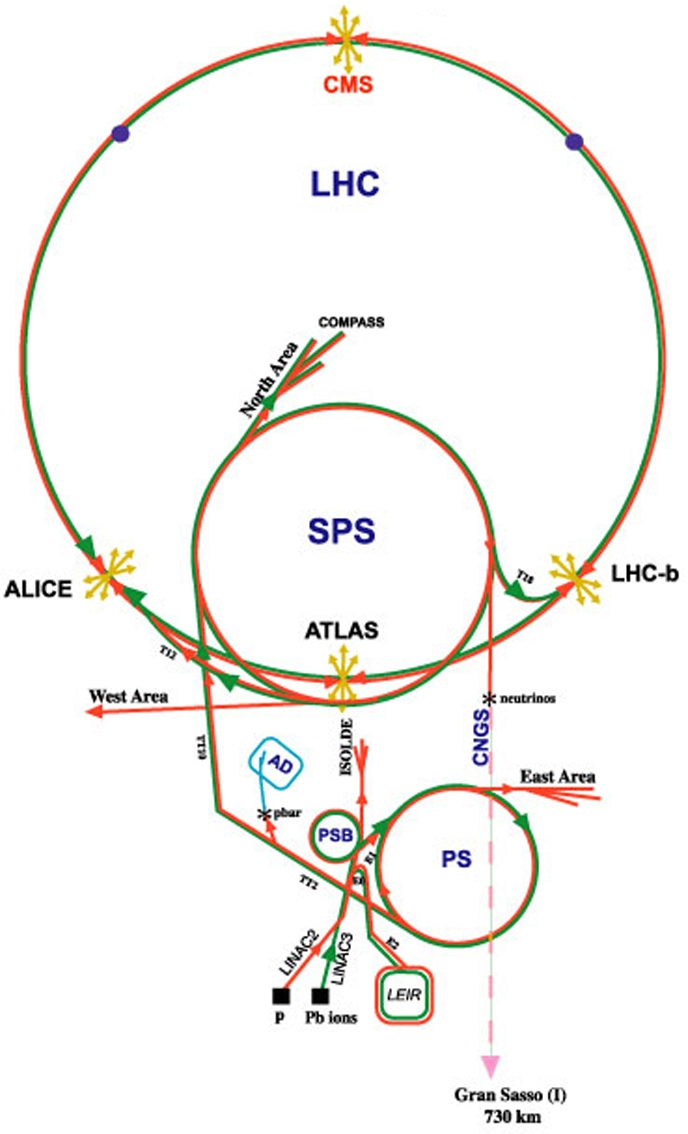
\includegraphics[width=0.4\columnwidth]{bilder/lhc}%
\caption{Schematische Skizze des LHC und seiner Vorbeschleuniger \cite{Hoehle:Diplom}.}%
\label{fig:lhc}%
\end{figure}
Die Designluminosit�t des LHC betr�gt 10$^{34}$\,cm$^{-2}$s$^{-1}$. Die wesentlichen Charakteristika des Beschleunigers bei Designluminosit�t und -energie sind in Tabelle~\ref{tab:lhc} zusammengefasst. \\
Diese Arbeit befasst sich mit der Analyse von Daten, die im Jahre 2011 bei einer Schwerpunktsenergie von 7 TeV genommen worden sind. In diesem Jahr wurden maximal \protect\linebreak{1,45 $\cdot$ 10$^{11}$} Protonen zu einem Paket zusammengefasst, und maximal 1380 Pakete waren gleichzeitig im Beschleuniger vorhanden. Diese hatten einen zeitlichen Abstand zueinander von 50\,ns. Abbildung~\ref{fig:lumi2012} zeigt die Entwicklung von instantaner und integrierter Luminosit�t des LHC im Jahre 2011. Am Ende des Jahres wurde eine integrierte Luminosit�t von 5,5\,fb$^{-1}$ erreicht.
\begin{table}
\caption{Design-Kenngr��en des LHC bei Proton-Proton-Betrieb \cite{LHC:Design1}.}
\centering
\vspace{0,2 cm}
\begin{tabular}{lrl}
\hline
\textbf{Eigenschaft} & \textbf{Wert} & \textbf{Einheit}	 \\
\hline
Umfang des Beschleunigers & 26,66 & km  \\
Umlauffrequenz & 11,2 & kHz \\
Schwerpunktsenergie & 14 & TeV \\
Energie pro Proton & 7 & TeV \\
Energie pro Strahl & 362 & MJ \\
Strahlstrom & 0,582 & A \\
Luminosit�t & 1,0 $\cdot$ 10$^{34}$ & cm$^{-2}$s$^{-1}$ \\
Teilchenpakete pro Strahl & 2808 & \\
Protonen pro Teilchenpaket & 1,15 $\cdot$ 10$^{11}$ & \\
Frequenz der Paketkollisionen & 40 & MHz \\
Kreuzungswinkel der Strahlen am IP & 285 & $\mu$rad \\
Radius des Strahls am IP & 16,7 & $\mu$m \\
L�nge eines Teilchenpaketes & 7,55 & cm \\
\hline
\end{tabular}
\label{tab:lhc}
\end{table}
\begin{figure}%
\centering
\begin{subfigure}[b]{0.4\textwidth}
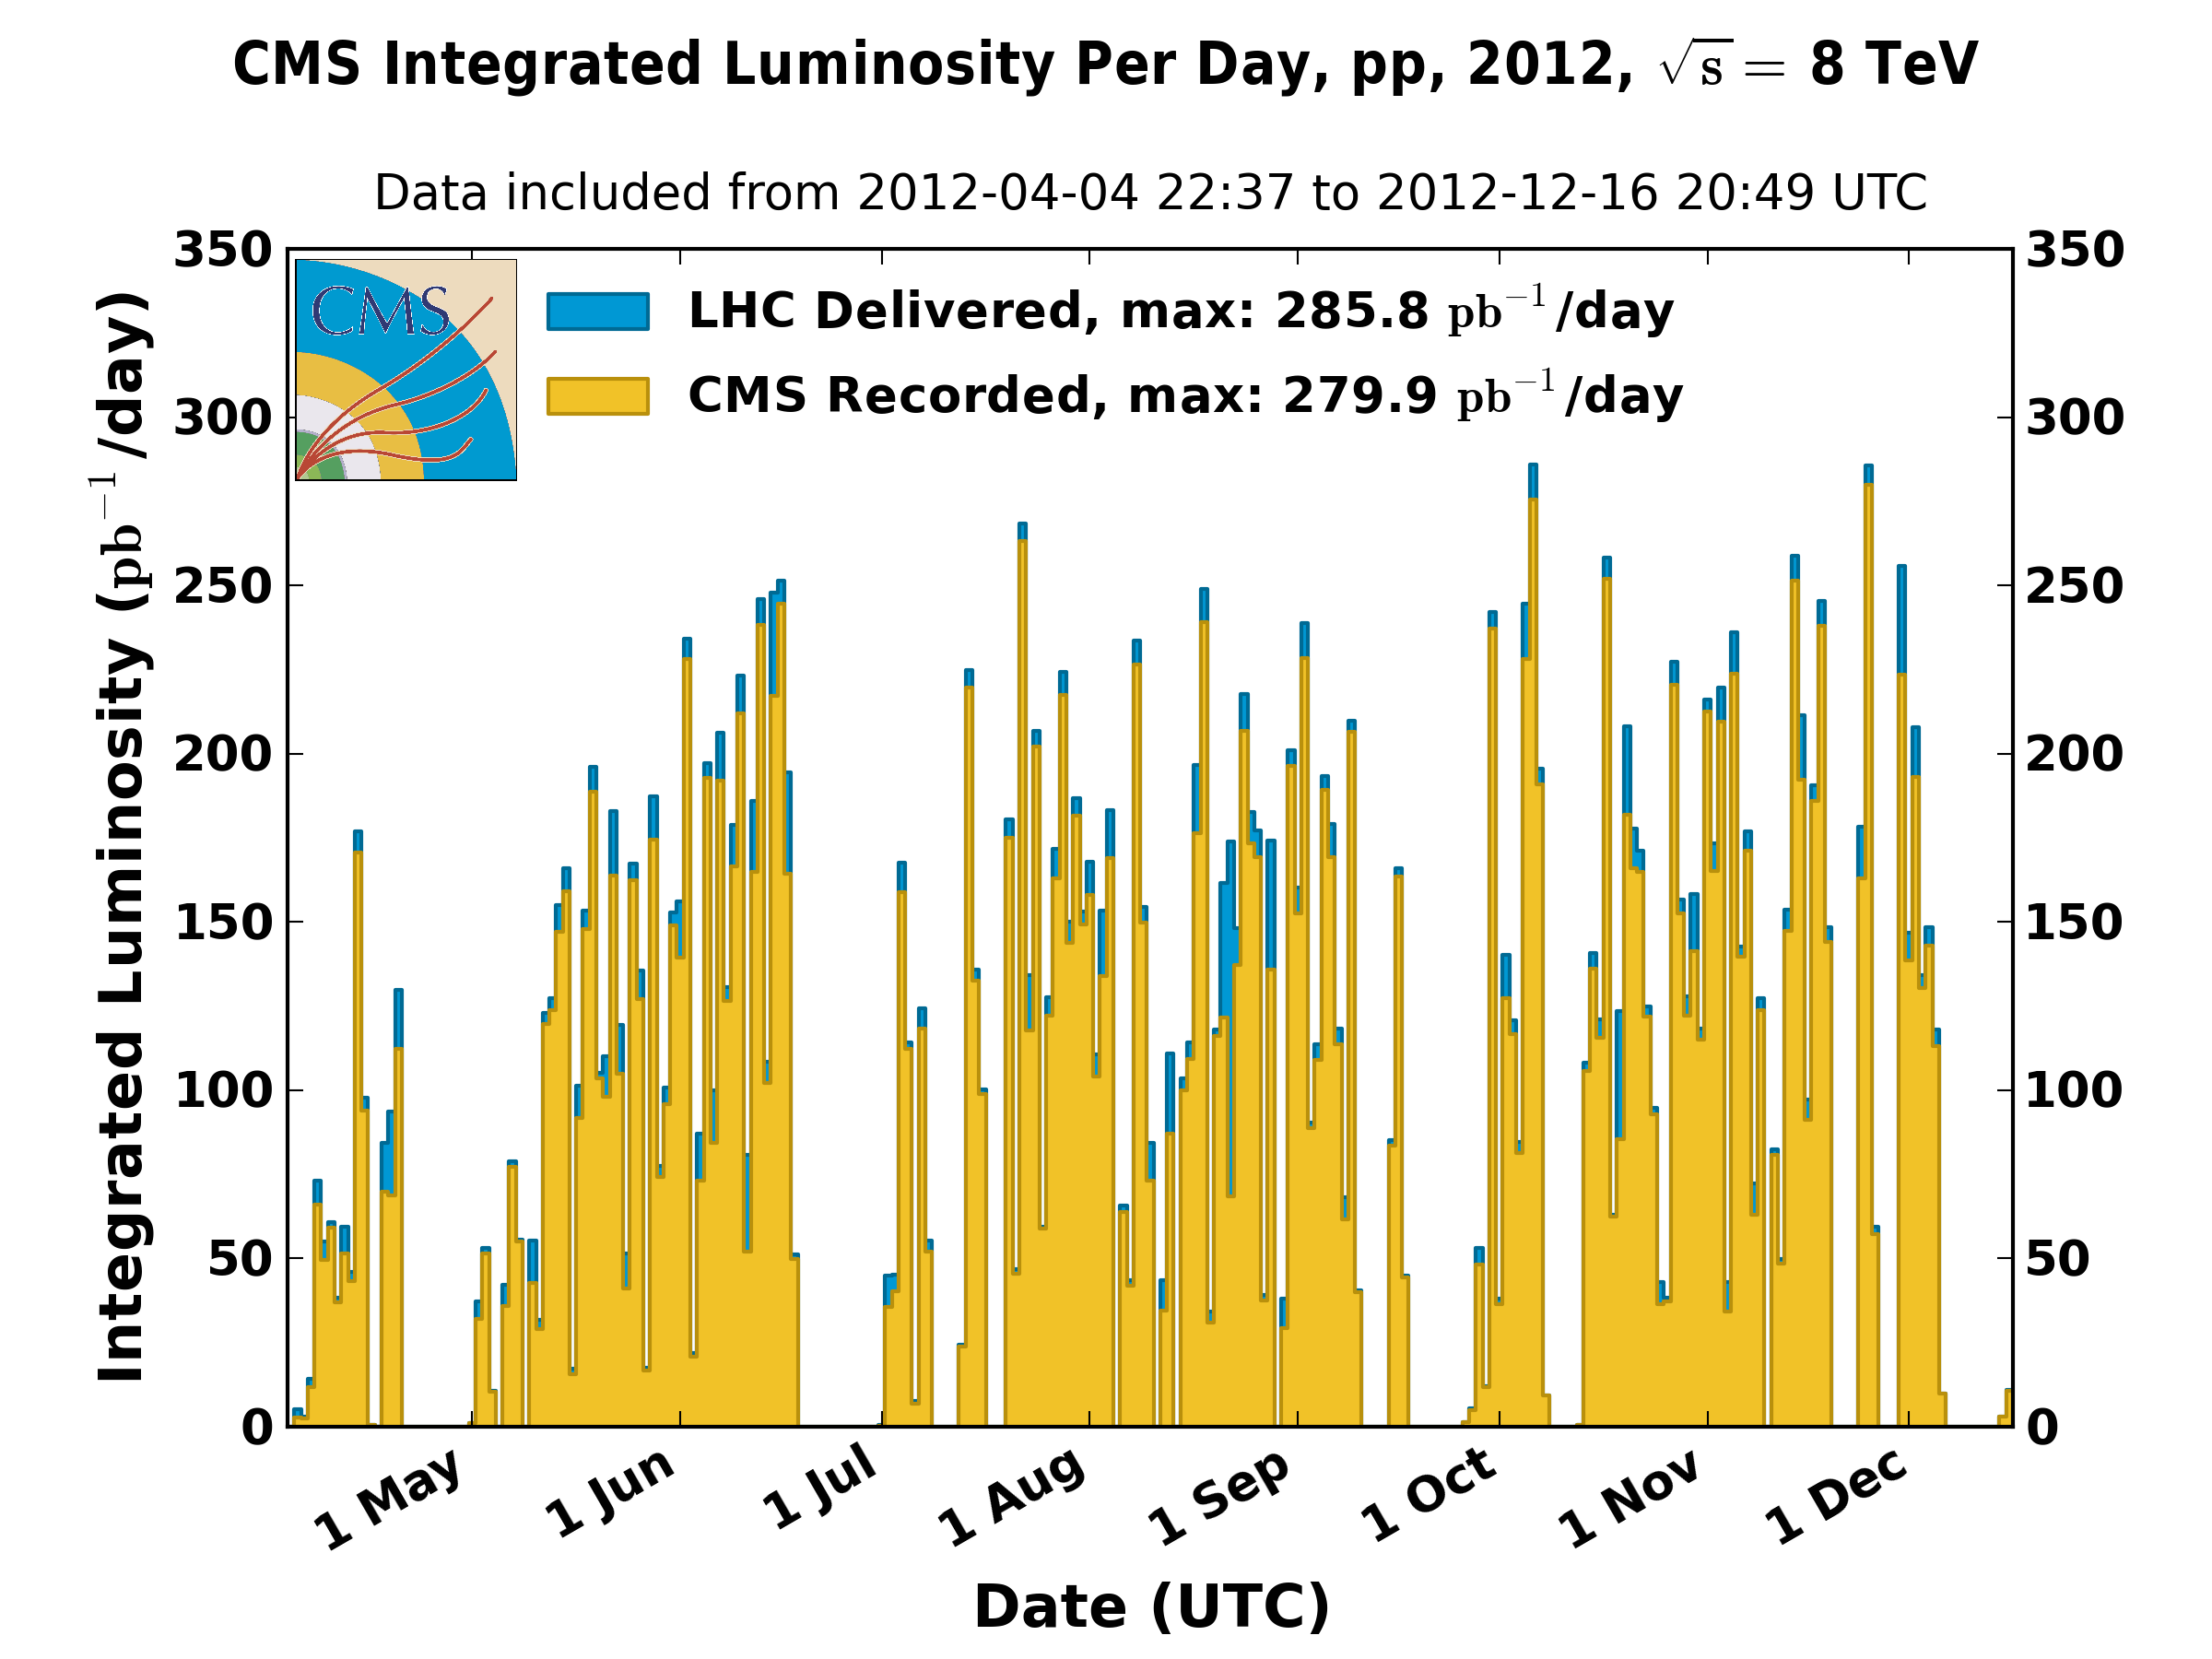
\includegraphics[width=\textwidth]{bilder/lumi2012}%
\end{subfigure}
\hspace{0.1\textwidth}
\begin{subfigure}[b]{0.4\textwidth}%
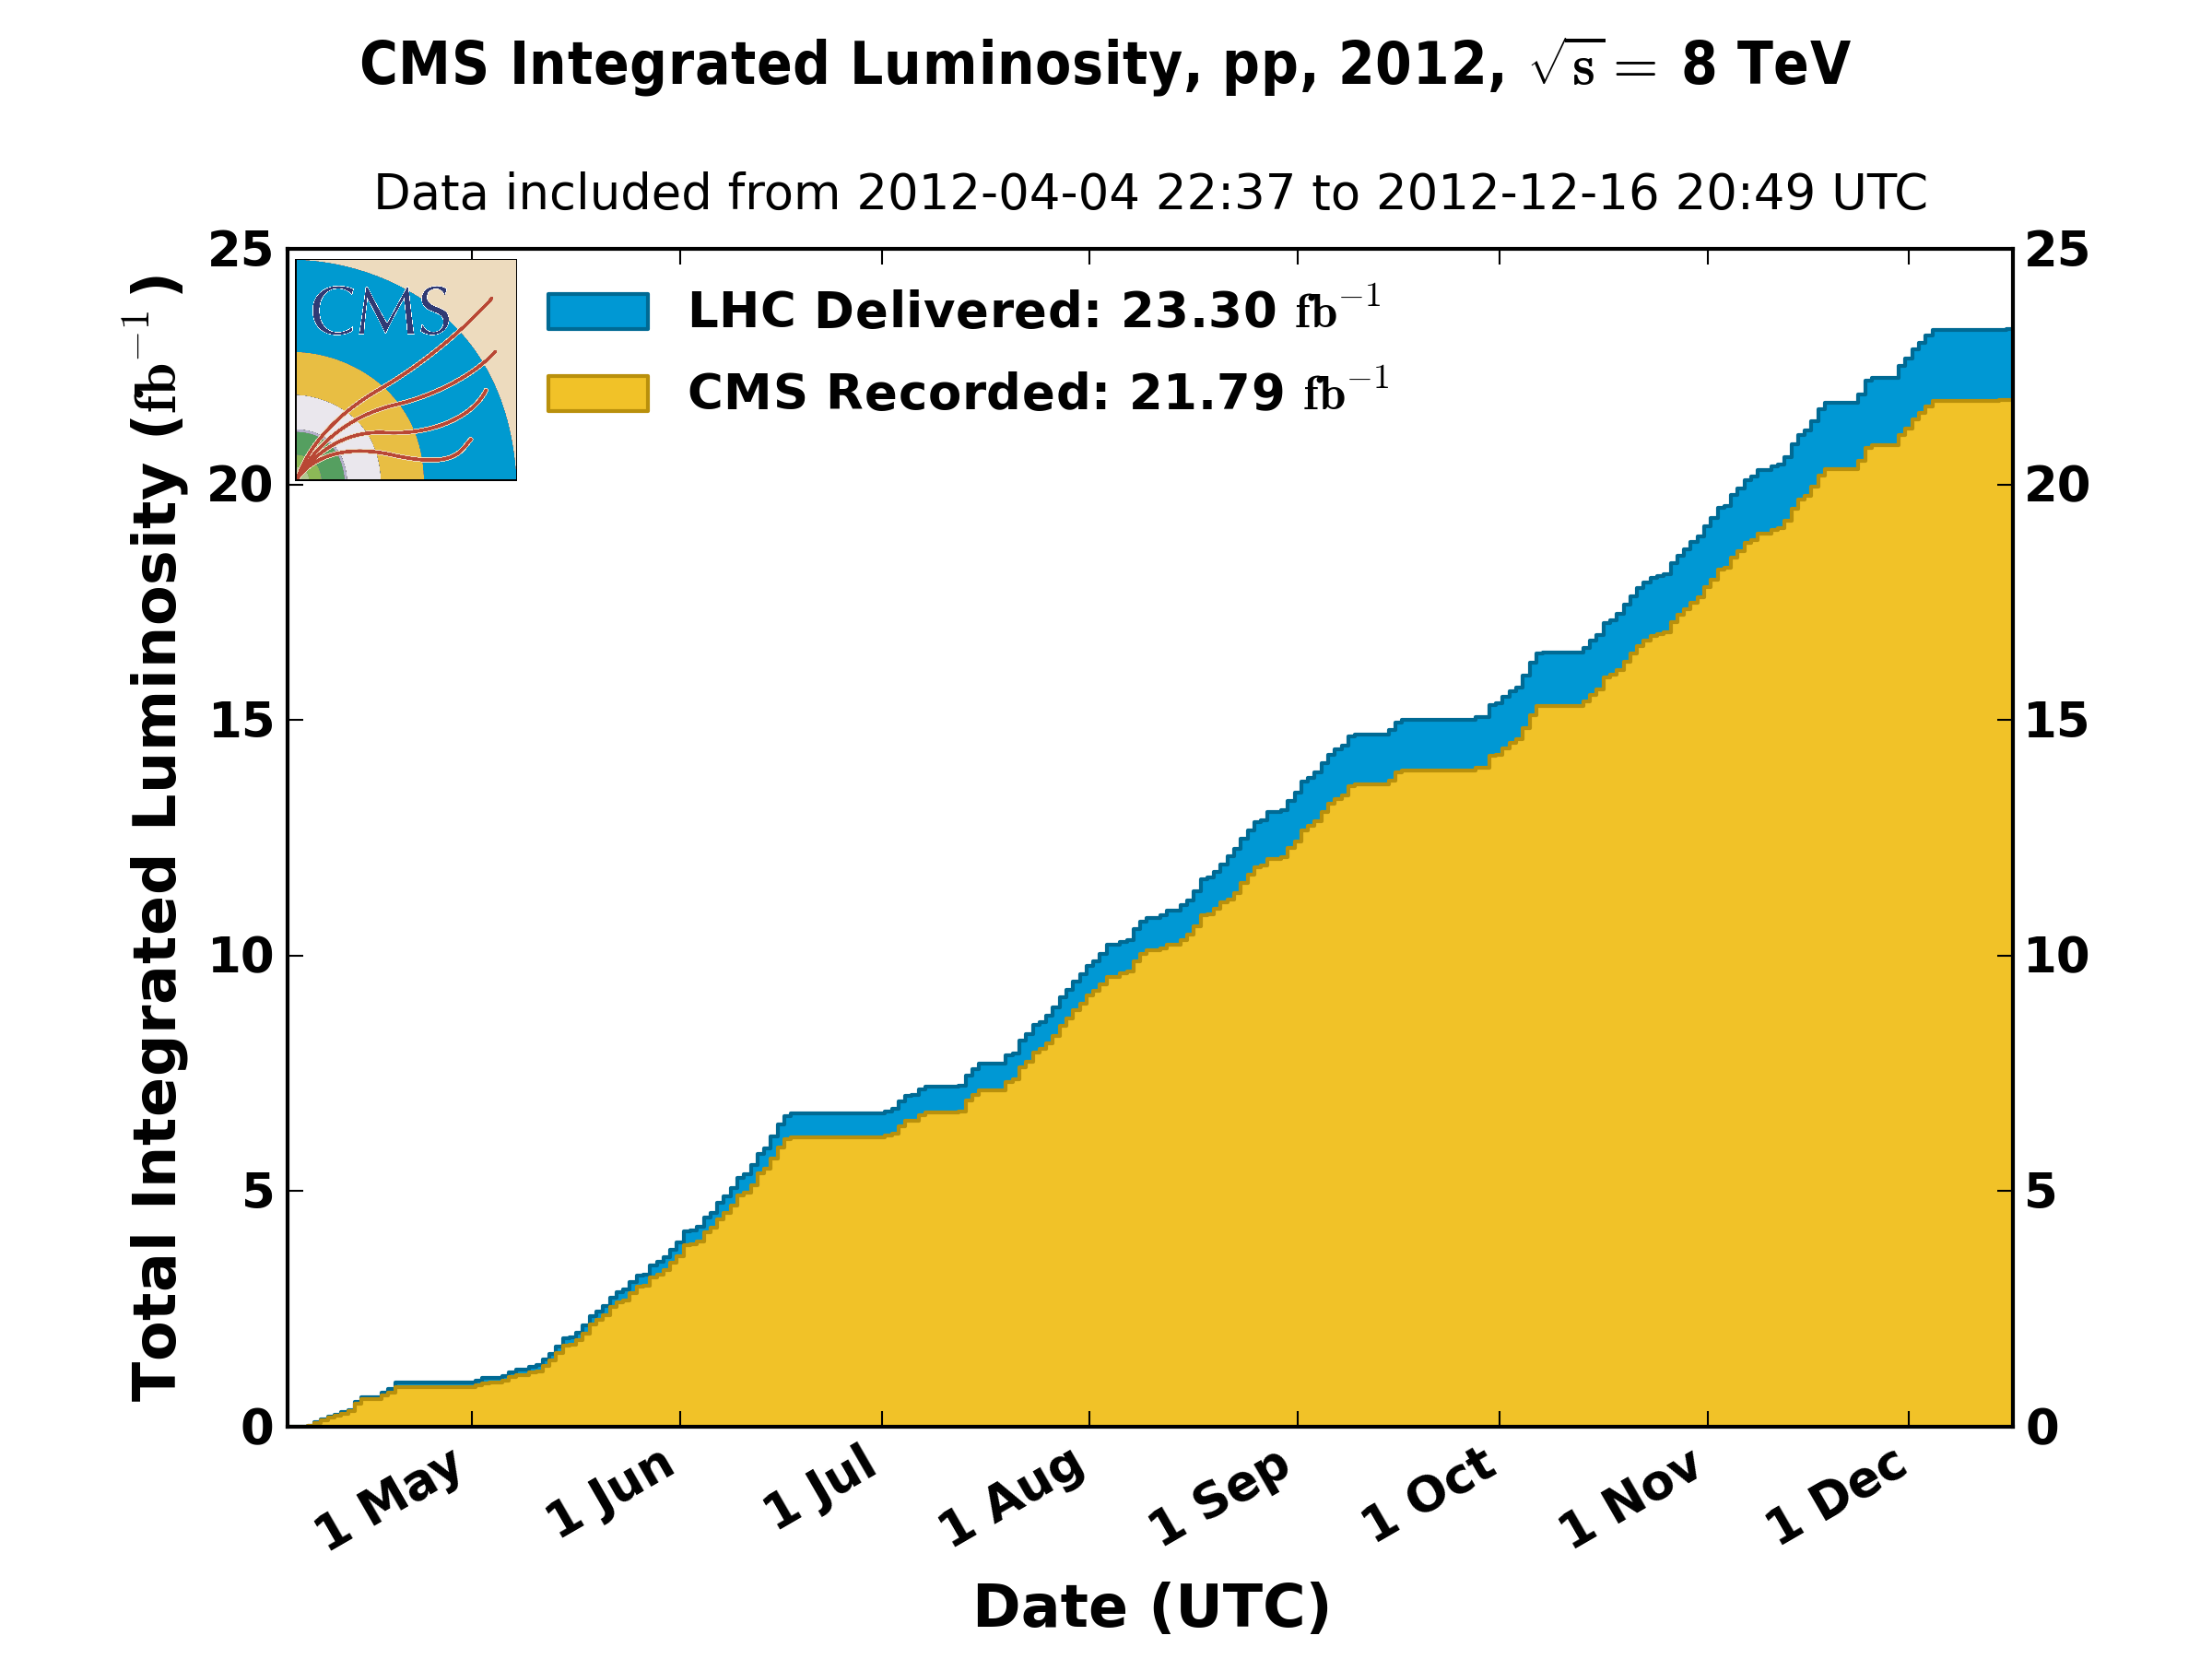
\includegraphics[width=\textwidth]{bilder/intlumi2012}%
\end{subfigure}
\caption{Zeitlicher Verlauf der maximalen (links) und totalen integrierten Luminosit�t (rechts) am CMS-Experiment in 2012 \cite{CMS:Lumiresults}.}%
\label{fig:lumi2012}%
\end{figure}

\section{Der CMS-Detektor}
\label{sec:detektor}

Der CMS-Detektor ist ein sogenannter Vielzweckdetektor, das hei�t er bildet einen Kompromiss aus Generalit�t auf der einen, sowie Spezialisierung auf besonders interessante physikalische Untersuchungen auf der anderen Seite. Der Name \enquote{Compact Muon Solenoid} (CMS) beschreibt, auf welche Aspekte beim Design des Detektors besonderer Wert gelegt wurde. \\
Der CMS-Detektor ist zylindrisch aufgebaut, 21,6\,m lang, hat einen Durchmesser von 14,6\,m und eine Masse von 12.500\,t. Trotzdem bezeichnet man den Detektor auf Grund seiner Bauweise mit wenigen Zwischenr�umen zwischen den einzelnen Komponenten als \enquote{kompakt}. Dadurch wird zum einen eine optimale Ausnutzung des Magnetfeldes zur Impulsmessung gew�hrleistet, zum anderen verringert sich die Wahrscheinlichkeit, dass Teilchen den Detektor undetektiert durch nicht abgedeckte Gebiete verlassen. \\
Eine der wesentlichen Anforderungen an den CMS-Detektor ist eine sehr gute Myonrekonstruktion. Myonen geben auf Grund ihrer hohen Masse kaum Bremsstrahlung ab, bilden demnach keine elektromagnetischen Schauer und durchdringen den gesamten Detektor. Dadurch k�nnen sie sehr gut identifiziert werden. Mit seinen leistungsf�higen Spurdetektoren und das Myonkammersystem kann der CMS-Detektor diese Anforderungen sehr gut erf�llen. \\
Das letzte namensgebende Element des Detektors ist der Solenoidmagnet, der in den Detektor integriert ist. Er erreicht eine Feldst�rke von bis zu 3,8\,T und kann dadurch auch bei hochenergetischen Teilchen deren Trajektorien derart kr�mmen, dass Ladung und idealerweise auch der Impuls des Teilchens bestimmt werden k�nnen. So ist eine der Hauptanforderungen an den CMS-Detektor erf�llt, die M�glichkeit, die Ladung von Myonen mit einem Transversalimpuls von bis zu 1\,TeV eindeutig bestimmen zu k�nnen \cite{Coll:CMSExperiment}. \\
\begin{figure}%
\centering
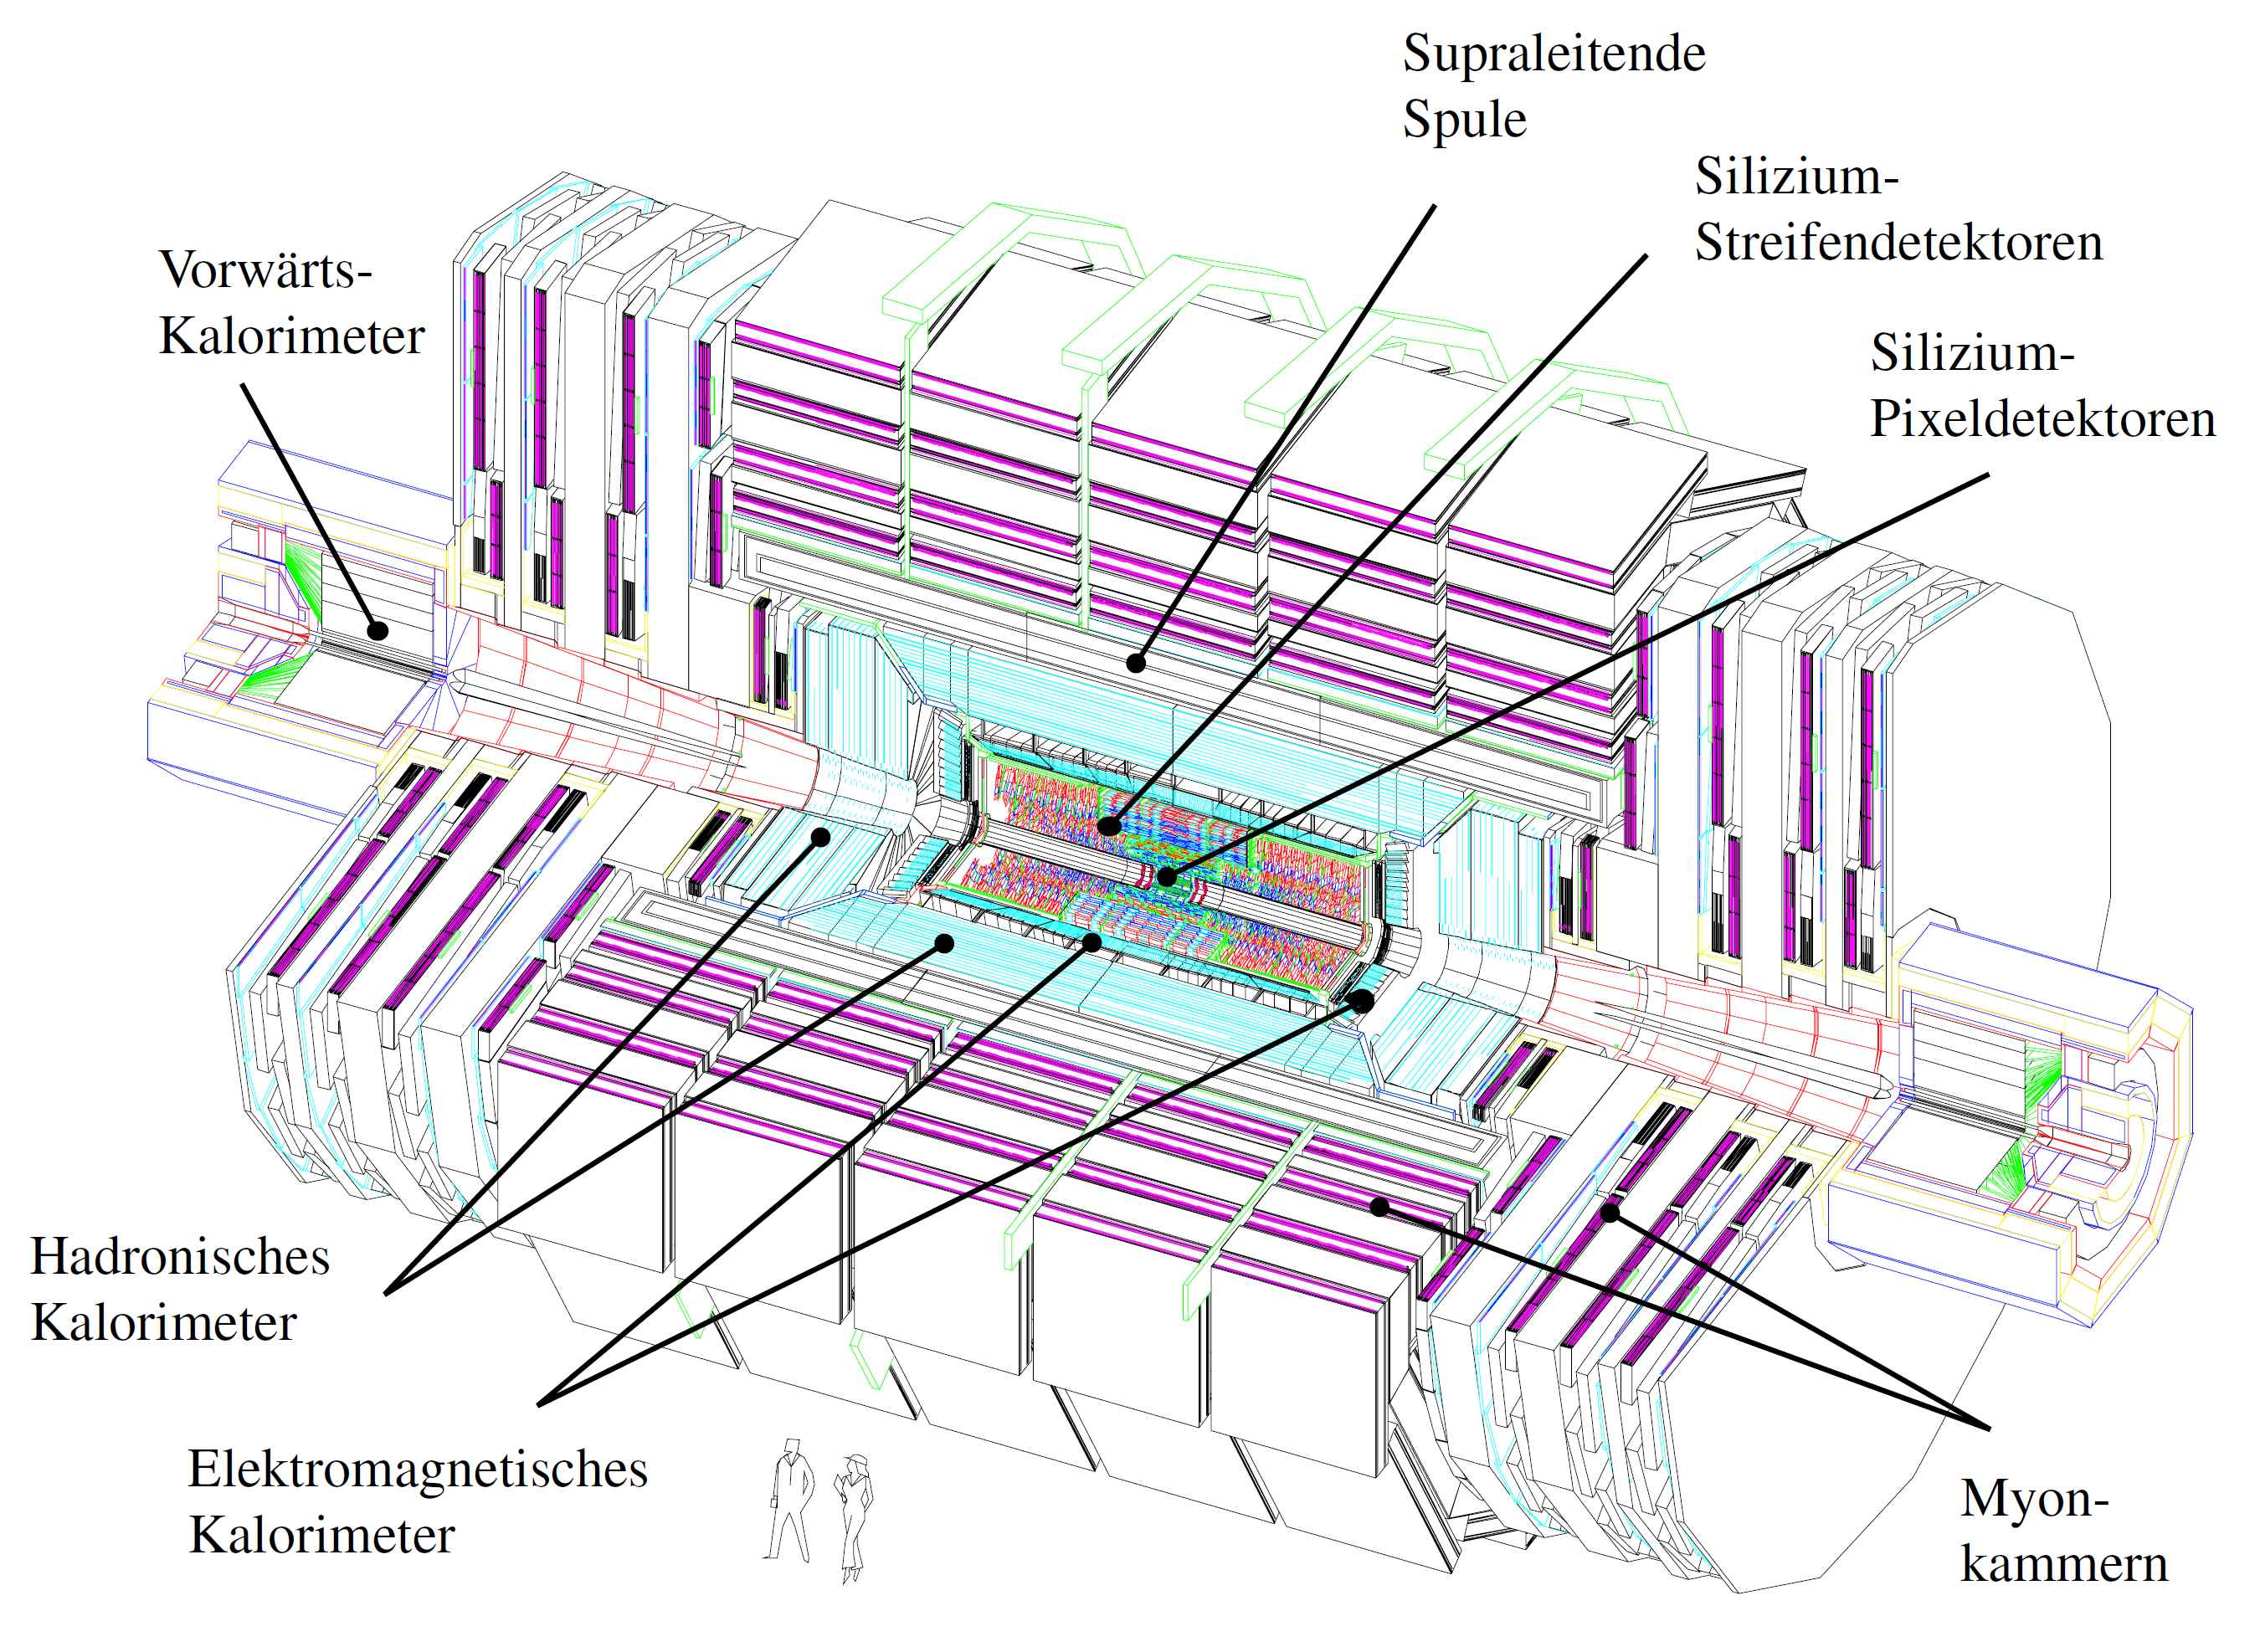
\includegraphics[width=0.6\columnwidth]{bilder/detektor.png}%
\caption{Schematische Skizze des CMS-Detektors \cite{Coll:CMSExperiment}.}%
\label{fig:detektor}%
\end{figure}
Eine Skizze des CMS-Detektors ist in Abbildung \ref{fig:detektor} gezeigt. Dort ist ein Teil des Detektors entfernt, um die einzelnen Komponenten sichtbar zu machen. Der \enquote{Interaction Point} stellt den Ursprung des Koordinatensystems dar, welches von der CMS-Kollaboration genutzt wird. Dabei zeigt die x-Achse zum Mittelpunkt des Beschleunigerrings, die y-Achse nach oben und die z-Achse entsprechend eines rechtsh�ndigen Koordinatensystems entlang der Strahlachse. Bei Angaben in Kugelkoordinaten wird der Polarwinkel $\Theta$ mit Startwert Null auf der positiven, sowie Endwert $\pi$ auf der negativen z-Achse verwendet. Der Azimuthalwinkel $\Phi$ ist in der x-y-Ebene senkrecht zum Strahl definiert. In der Teilchenphysik wird statt des Polarwinkels $\Theta$ h�ufig die Pseudorapidit�t $\eta$ genutzt,  da sie lorentzinvariant ist. Sie ist gegeben durch
\begin{equation}
\eta = - \ln \left\lbrack \tan \left(\frac{\Theta}{2}\right)\right\rbrack \ .
\end{equation}


\subsection{Die Silizium-Spurdetektoren}

Den innersten Kern des Detektors bilden die Spurdetektoren. Durch ihre unmittelbare N�he zum Kollisionspunkt befindet sich nur wenig Material zwischen dem Wechselwirkungspunkt und der Messsensorik. Dies bewirkt eine Verringerung der Vielfachstreuung und es wird eine hochpr�zise Messung erm�glicht. Aufgrund dieser genauen Spurmessungen erreicht man eine sehr gute Rekonstruktion der prim�ren und sekund�ren Vertizes. Dies ist notwendig, um die im Mittel bis zu 20 Teilchenkollisionen pro Paket trennen zu k�nnen (\enquote{Pile-up rejection}) und eine gute Rekonstruktion der Sekund�rvertizes zu erm�glichen. Dies ist unter anderem wichtig f�r die Identifizierung von Jets aus b-Quarks (B-Tagging). \\
Die Spurdetektoren bestehen aus zwei verschiedenen Systemen, dem Pixeldetektor und dem Streifendetektor, deren Funktionsweise und Performanz in den folgenden Abschnitten beschrieben werden. Der Pixeldetektor erreicht eine bessere Aufl�sung, beschr�nkt sich jedoch aus Kostengr�nden nur auf den inneren Bereich des Spurdetektors. \\
Die gro�e N�he der Silizium-Spurdetektoren zum Wechselwirkungspunkt hei�t, dass die Detektoren einem sehr hohen Teilchenfluss ausgesetzt werden. Um die dadurch verursachten Sch�den im Silizium-Gitter zu verringern, werden die Siliziummodule auf eine Temperatur von -10\,�C herabgek�hlt. Die Laufzeit des Pixeldetektors erreicht somit 2 Jahre bei Designluminosit�t, der Streifendetektor ist f�r eine Lebensdauer von 10 Jahren ausgelegt.

\begin{figure}%
\centering
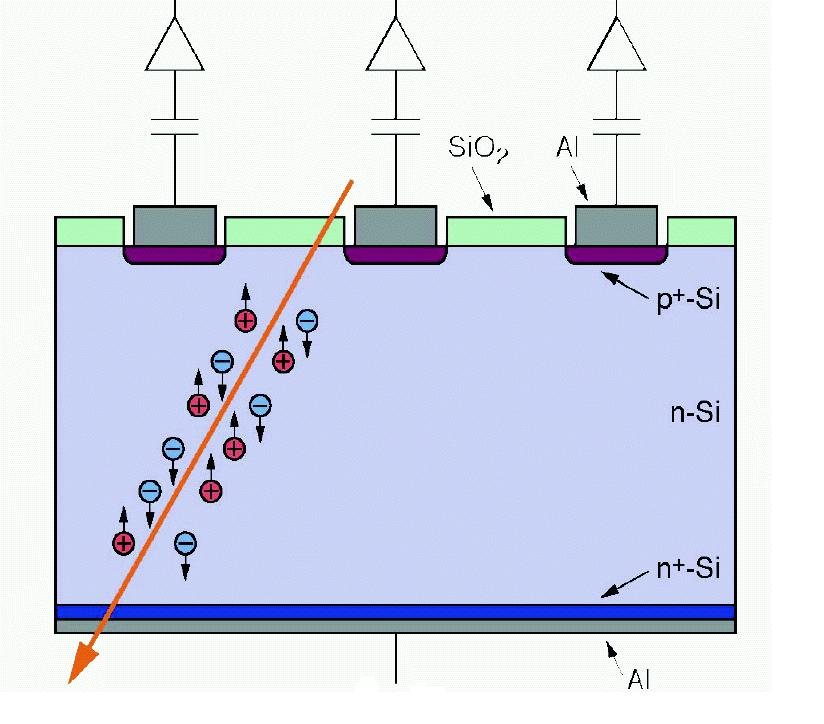
\includegraphics[width=0.4\columnwidth]{bilder/halbleiterdetektor.png}%
\caption{Skizze zur Funktionsweise eines Halbleiterdetektors \cite{Kuessel:Diplom}.}%
\label{fig:halbleiterdetektor}%
\end{figure}

\subsubsection*{Funktionsweise eines Spurdetektors}

Die Spurdetektoren im CMS-Experiment sind Silizium-Halbleiterdetektoren. Beim Durchgang eines geladenen Teilchens durch die Verarmungszone eines p-n-�bergangs werden entlang seiner Spur Ladungen erzeugt. Diese flie�en zur Anode bzw. Kathode ab und erzeugen dort einen elektrischen Strompuls, siehe Abbildung~\ref{fig:halbleiterdetektor}. Es l�sst sich anhand des Kr�mmungsradius $r$ und dem Magnetfeld $B$ der Teilchenimpuls bestimmen:

\begin{equation}
p = qvBr
\end{equation}
Der Kr�mmungsradius $r$ wird �ber die Sagitta bestimmt. Daher ist die Messgenauigkeit proportional zum Teilchenimpuls.

\subsubsection*{Der Pixeldetektor}

Der Pixeldetektor ist unterteilt in den Barrel Pixel (BPIX) und den Forward Pixel (FPIX), siehe Abbildung~\ref{fig:pixeldetektor}. Der BPIX besteht aus drei jeweils 53\,cm langen zylindrischen Lagen mit Radien von 4,4\,cm, 7,3\,cm und 10,2\,cm. Die beiden FPIX haben einen Durchmesser von 30\,cm und bestehen aus jeweils 2 Scheiben, die bei $\left|z\right| = $ 34,5\,cm und $\left|z\right| = $ 46,5\,cm installiert sind. Die insgesamt 66 Millionen Pixel bedecken eine Fl�che von 1\,m$^{2}$ und erstrecken sich bis $\left|\eta\right| = $ 2,4. Die einzelnen Pixel haben eine Ausdehnung von $100 \times 150\, \mu$m$^{2}$. Diese ist so gew�hlt, dass �quivalente Aufl�sungen in der $r-\Phi-$Ebene sowie in $z-$Richtung erreicht werden. Durch die Lorentzkraft verteilen sich die im Silizium freigesetzten Ladungen �ber mehrere Pixel. Durch eine analoge Auslese der einzelnen Pixel kann dann �ber eine Gewichtung benachbarter Messwerte eine r�umliche Aufl�sung von 15 - 20\,$\mu$m erreicht werden.

\begin{figure}[b]%
\centering
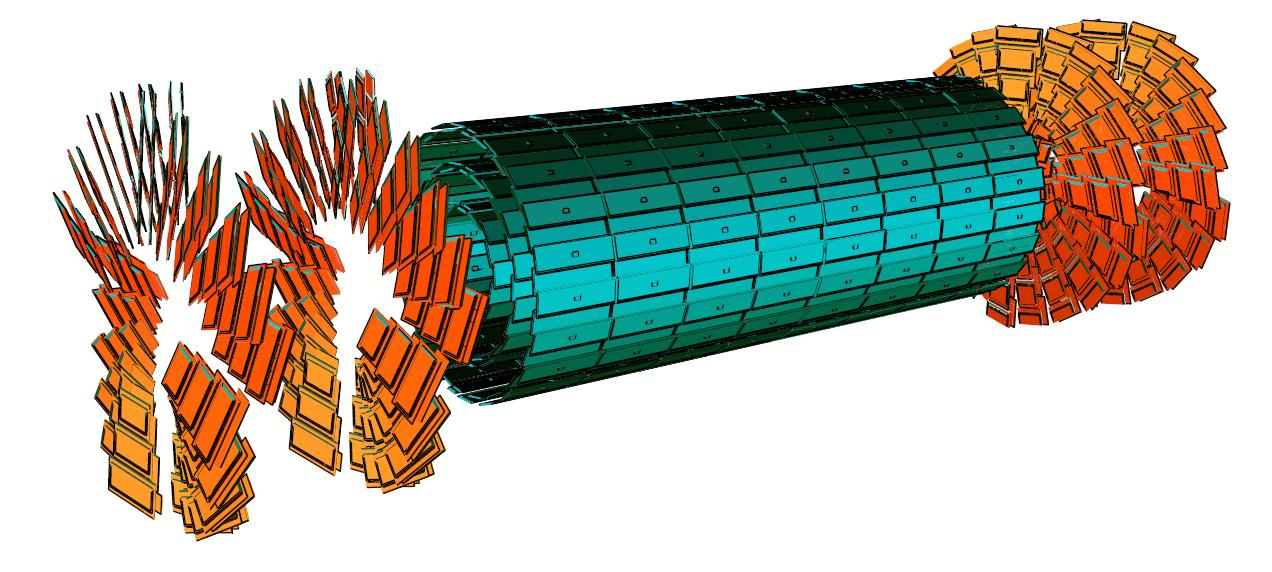
\includegraphics[width=0.7\columnwidth]{bilder/pixeldetektor.png}%
\caption{Schematische Skizze des Pixeldetektors. Mittig die einzelnen Module des BPIX und an deren Enden die Module des FPIX \cite{Kuessel:Diplom}.}%
\label{fig:pixeldetektor}%
\end{figure}

\subsubsection*{Der Streifendetektor}

Der Streifendetektor schlie�t sich unmittelbar an den Pixeldetektor an. Er l�sst sich, wie in Abbildung~\ref{fig:streifendetektor} dargestellt, in vier Bereiche einteilen: Tracker Inner Barrel (TIB), Tracker Inner Disks (TID), Tracker Outer Barrel (TOB) sowie Tracker Endcap (TEC), die sich durch die Anordnung und Art ihrer Module unterscheiden. TIB und TOB sind zylindrisch um die Strahlachse angeordnet, TID und TEC bilden Endkappen senkrecht zur Strahlrichtung. Der gesamte Detektor hat einen Radius von 1,1\,m bei einer L�nge von 5,8\,m. Damit ergibt sich eine aktive Detektorfl�che von 198\,m$^{2}$ und eine Abdeckung von $\left|\eta\right| < $ 2,5.\\
Insgesamt sind 9,3 Millionen Siliziumstreifen auf 15.148 Detektormodulen installiert. Neben den einseitigen gibt es auch doppelseitige Module, um die Spuraufl�sung zu erh�hen. Diese bestehen aus zwei einseitigen Modulen, deren Siliziumstreifen unter einem Winkelversatz von 5,7\,� R�cken an R�cken angebracht sind. Dadurch wird eine Ortsaufl�sung von 23-53\,$\mu$m in der $r-\Phi-$Ebene und 230-530\,$\mu$m in $z-$Richtung erm�glicht. Die L�nge der Sensoren nimmt mit steigendem Radius zu, damit ihre Okkupanz gleich bleibt. So wird jedoch gleichzeitig das Signal-zu-Rauschen-Verh�ltnis ver�ndert, dies wird durch eine ansteigende Dicke der Sensoren ausgeglichen. Diese betr�gt innen 320\,$\mu$m und nimmt nach au�en bis auf 500\,$\mu$m zu.

\begin{figure}[h]%
\centering
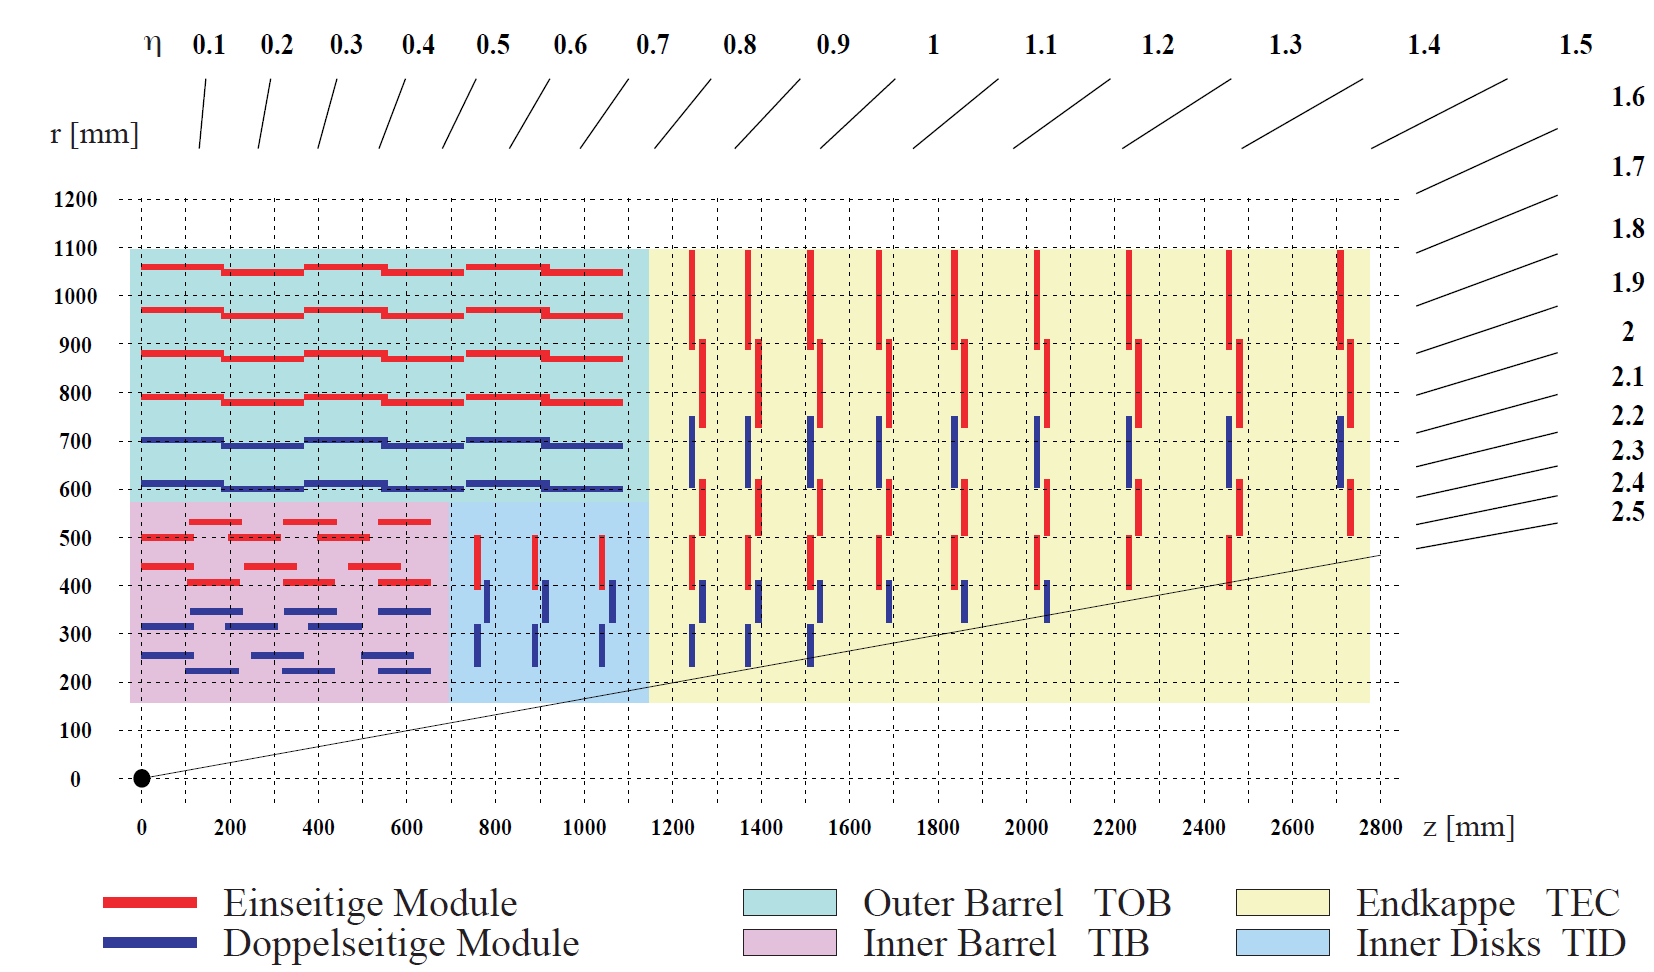
\includegraphics[width=0.7\columnwidth]{bilder/streifendetektor.png}%
\caption{Schema des Streifendetektors \cite{Hegner:Diplom}.}%
\label{fig:streifendetektor}%
\end{figure}

\subsection{Die Kalorimeter}

Das Kalorimetersystem des CMS-Experimentes setzt sich aus einem elektromagnetischen Kalorimeter (ECAL) und einem hadronischen Kalorimeter (HCAL) zusammen. Dabei schlie�t sich das ECAL direkt an den Silizium-Streifendetektor an, radial dahinter angebracht ist das HCAL. In den Kalorimetern sollen alle Teilchen gestoppt und ihre Energie dabei m�glichst genau vermessen werden. Davon ausgenommen sind Myonen, welche die Kalorimeter passieren und im Myonsystem n�her untersucht werden sowie Neutrinos, die ausschlie�lich der schwachen Wechselwirkung unterliegen und so vom CMS-Detektor gar nicht direkt beobachtet werden k�nnen, sondern nur indirekt �ber fehlende transversale Energie. \\
Im ECAL werden haupts�chlich elektromagnetisch und wenig stark wechselwirkende Teilchen vermessen, also Photonen und Elektronen. Aufgabe des HCAL ist die Detektion aller stark wechselwirkenden Teilchen. Diese sind Mesonen und Baryonen, die aus Hadronisierungsprozessen hervorgegangen sind.

\subsubsection*{Das elektromagnetische Kalorimeter}

Elektronen und Photonen werden im ECAL durch zwei Prozesse ineinander umgewandelt und dabei abgebremst: Bremsstrahlung ($e \rightarrow e\gamma$) und Paarbildung ($\gamma \rightarrow e^{+}e^{-}$). Dabei ist die Strahlungsl�nge bei Bremsstrahlung etwa gleich der Wechselwirkungsl�nge f�r Paarbildung. Es gibt mehrere Kenndaten, die einen so entstehenden Teilchenschauer beschreiben:
\begin{itemize}
	\item Die Strahlungsl�nge $X_{0}$ bezeichnet die L�nge, nach der ein Elektron auf 1/e seiner urspr�nglichen Energie abgebremst wurde und ist charakteristisch f�r das Material, das im Kalorimeter verbaut wurde.
	\item Der Moli�re-Radius $R_{M}$ beschreibt die transversale Ausdehnung des Schauers und enth�lt 95\% der Energie des Ursprungsteilchens. Er ist in guter N�herung proportional zur Strahlungsl�nge.
	\item Der Teilchenschauer stoppt, wenn die Energie der Photonen unter die doppelte Elektronmasse (Ausbleiben der Paarerzeugung) und die Energie der Elektronen unter die kritische Energie $E_{C}$ (Ausbleiben der Bremsstrahlung) f�llt. F�r diese gilt:
	\begin{equation}
	E_{C} = \frac{E_{0}}{2^{n}},
	\end{equation}
	hierbei ist $E_{0}$ die Energie des Ursprungsteilchens und $n$ die Zahl der Strahlungsl�ngen bis zum Unterschreiten der kritischen Energie.
\end{itemize}
Die so entstandenen Teilchen werden durch einen Szintillator detektiert und von Photomultipliern ausgelesen. Deren Anzahl ist proportional zur Anfangsenergie $E_{0}$ des abzubremsenden Teilchens, somit ergibt sich eine Energieaufl�sung eines Kalorimeters von
\begin{equation}
\frac{\sigma(E)}{E} \propto \frac{1}{\sqrt{E}}.
\label{eq:energieaufloesung}
\end{equation}
Im ECAL des CMS-Experimentes werden Kristalle aus Blei-Wolframat (PbWO$_{4}$) verwendet, einem Metallglas, welches sowohl die einfallenden Teilchen effektiv abbremst als auch selbst als Szintillator dient. Es sind 61.200 Kristalle im Barrel-Bereich sowie jeweils 7.324 Kristalle in den Endkappen verbaut. PbWO$_{4}$ hat aufgrund seiner hohen Dichte eine sehr kurze Strahlungsl�nge $X_{0} = 0,89$\,cm und einen somit kleinen Moli�re-Radius \protect\linebreak{$R_{M} = 2,2$\,cm}. Es eignet sich somit sehr gut f�r die kompakte Bauweise des Kalorimeters. \\
Die verwendeten Kristalle haben eine Querschnittsfl�che von 22 $\times$ 22\,mm$^{2}$, also in der Gr��enordnung des Moli�re-Radius, und eine L�nge von 23\,cm. Dies entspricht 25,8 Strahlungsl�ngen. Das ECAL erreicht eine sehr hohe Granularit�t von 0,0175\,rad in $\eta$ und $\Phi$ im Barrel-Bereich und 0,05\,rad im Bereich der Endkappen. Durch diese hohe Granularit�t ist allerdings die Lichtausbeute pro MeV mit vier bis f�nf Photoelektronen gering, so dass das Lichtsignal der Szintillatoren verst�rkt werden muss und hohe Anforderungen an die verwendeten Photodioden und -trioden gestellt werden. Deswegen werden daf�r im Barrel-Bereich Lawinenphotodioden (Avalanche Photodiodes, APDs) aus Silizium genutzt. Diese wurden speziell f�r CMS entwickelt. In den Endkappen sind Vakuum-Phototrioden verbaut, die eine Quanteneffizienz von 22\% und eine maximale Verst�rkung bis 10,2 erreichen. \\
Die Energieaufl�sung des Kalorimeters kann wie folgt parametrisiert werden:
\begin{equation}
\frac{\sigma_{E}}{E} = \frac{2,8\%}{\sqrt{E}} \oplus \frac{12\%}{E} \oplus 0,3\% \quad(E \text{ in GeV})
\label{eq:}
\end{equation}
Hier ber�cksichtigt der erste Term die stochastischen Schwankungen aus Gleichung~\ref{eq:energieaufloesung}, der zweite Term alle Arten von Rauschen, darunter elektronisches Rauschen und Digitalisierungseffekte. Der dritte, konstante Term schlie�lich ber�cksichtigt Kalibrationsfehler und ist dominant bei hohen Energien.

\subsubsection*{Das hadronische Kalorimeter}

\begin{figure}%
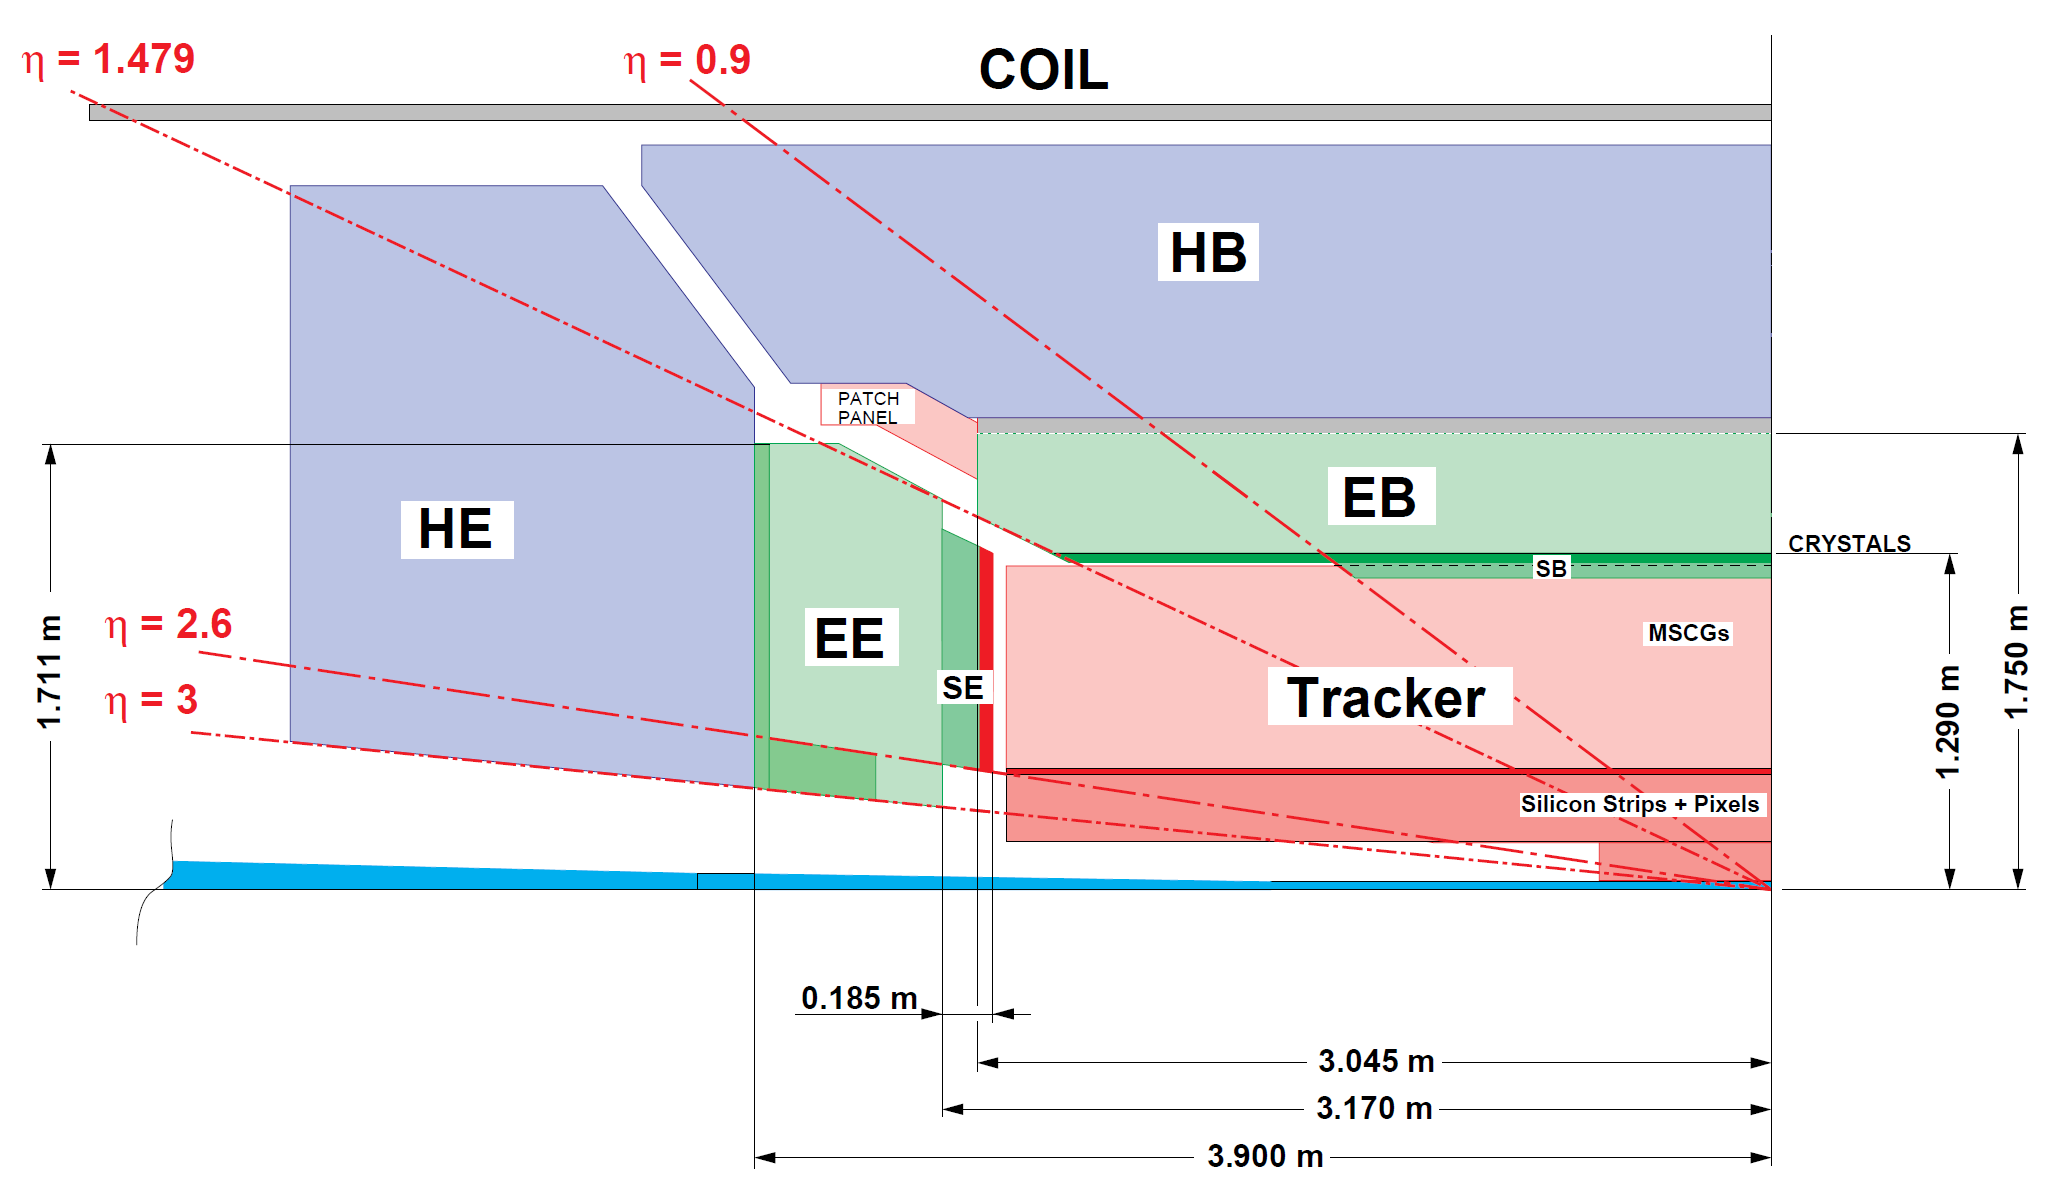
\includegraphics[width=\columnwidth]{bilder/kalorimeter}%
\caption{Anordnung des elektromagnetischen und hadronischen Kalorimeters. Gezeigt sind jeweils der Barrel- und Endkappenbereich \cite{Hoehle:Diplom}.}%
\label{fig:kalorimeter}%
\end{figure}

Auf das ECAL folgt in radialer Richtung unmittelbar das HCAL, das zum Gro�teil ebenfalls noch innerhalb des Solenoidmagneten liegt. Es ist aufgeteilt in die Teile Barrel (HB), Endkappen (HE) und Vorw�rtsbereich (HF), siehe Abbildung~\ref{fig:kalorimeter} und~\ref{fig:kalorimeter2}. Die zentralen Module decken einen Bereich von $\left|\eta\right| \leq 3$ ab, der anschlie�ende Vorw�rtsbereich geht bis $\left|\eta\right| = 5$. \\
Das hadronische Kalorimeter ist als Sampling-Kalorimeter konstruiert, das absorbierende Schauermaterial ist also physikalisch vom Detektormaterial getrennt. Als Absorber wird hier Messing und als detektierendes Material Plastikszintillatoren verwendet, die mittels einer wellenl�ngenschiebenden Faser ausgelesen werden. Der Vorw�rtsbereich des HCAL besteht aufgrund der hohen Strahlungsbelastung in Strahlrohrn�he aus einer Quarz-/Eisen-Struktur, in der die Teilchen durch Cerenkov-Licht nachgewiesen werden. Er ist 6\,m hinter den Endkappen angebracht, au�erhalb des Myonsystems, siehe Abbildung~\ref{fig:kalorimeter2} und dient unter anderem der Messung fehlender transversaler Energie durch Neutrinos. Ebenso au�erhalb des Solenoidmagneten befindet sich im zentralen Bereich das Outer Calorimeter (HO, Abb.~\ref{fig:kalorimeter2}). Es dient der Detektion so genannter \enquote{Punch-thrus}. Das sind entweder besonders hochenergetische Hadronen oder Hadronen, die erst sp�t aufschauern. Diese k�nnen im HCAL nicht hinreichend gestoppt werden und somit auch Eintr�ge im Myonsystem hinterlassen. Das HO kann somit verhindern, dass die Punch-thrus als Myonen miss-rekonstruiert werden. Die Dicke des HCAL erreicht damit etwa 12 Strahlungsl�ngen. Zusammen mit dem ECAL betr�gt die Energieaufl�sung des HCAL
\begin{equation}
\frac{\sigma(E)}{E} = \frac{1}{\sqrt{E}} \oplus 0,045 \ .
\end{equation}

\begin{figure}%
\centering
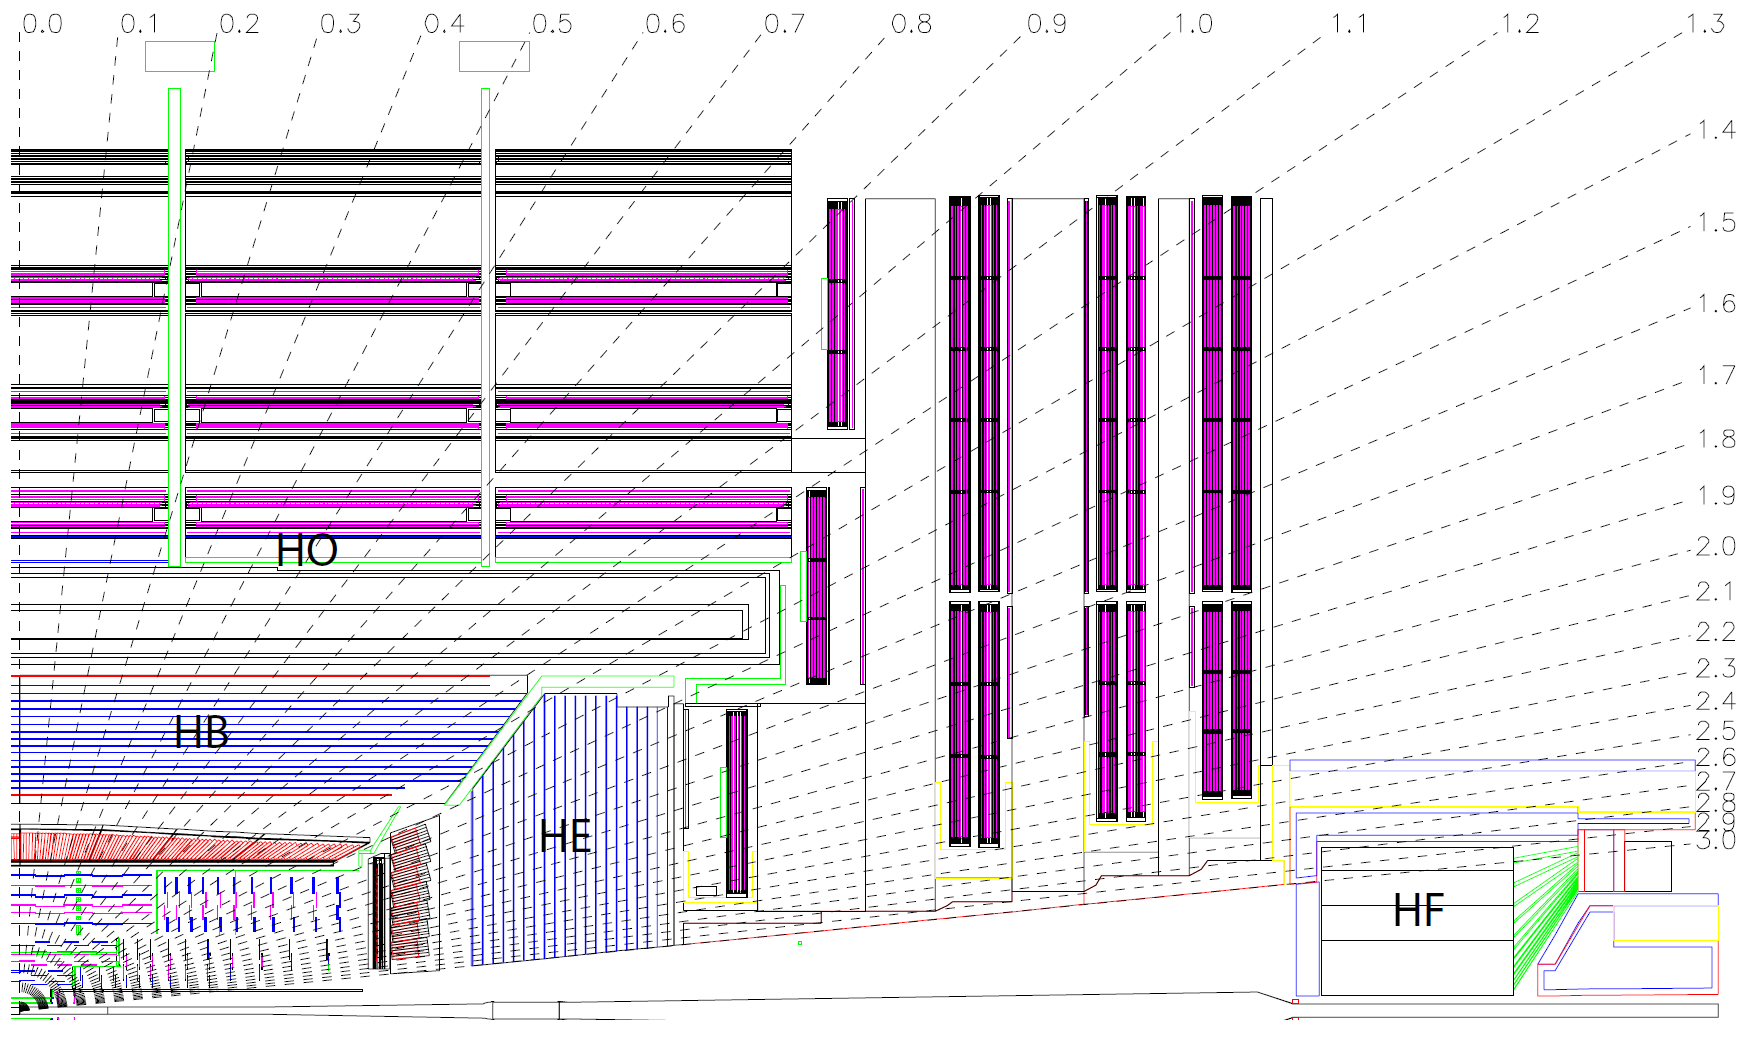
\includegraphics[width=0.7\columnwidth]{bilder/kalorimeter2}%
\caption{�bersicht des CMS-Detektors mit Outer Calorimeter (HO) und Vorw�rtskalorimeter (HF) \cite{Coll:CMSExperiment}.}%
\label{fig:kalorimeter2}%
\end{figure}

\subsection{Der Solenoidmagnet}

Der f�r den Detektor namensgebende Solenoidmagnet erzeugt ein Magnetfeld von bis zu 3,8\,T. Diese hohe Feldst�rke ist notwendig, um die Bahnen der bei Schwerpunktsenergien von bis zu 14\,TeV entstehenden hochenergetischen Teilchen ausreichend zu kr�mmen. Das Feld wird mittels einer supraleitenden Niob-Titan-Spule erzeugt. Diese ist auf 4,5\,K abgek�hlt und besitzt 2168 Windungen. Der umlaufende Strom von 19,5\,kA erzeugt ein Feld der Energie 2,7\,GJ. Es wurde Wert darauf gelegt, die massive Magnetspule so weit wie m�glich au�en im Detektor anzuordnen, da sie die Messung auf Grund von Vielfachstreuung der Teilchen verf�lscht. Im CMS-Detektor ist der Solenoidmagnet im Abstand von 5,9\,m von der Strahlachse angebracht und erreicht eine L�nge von 12,9\,m.

\subsection{Die Myonkammern}

An den Solenoiden schlie�t sich das Myonsystem als letzte Detektorkomponente an. Es ist au�erhalb des Solenoidmagneten in dessen R�ckf�hrjoch integriert, so dass auch hier ein Magnetfeld existiert, das jedoch dem im Inneren des Detektors entgegengerichtet ist und eine Feldst�rke von 2\,T aufweist. Somit wird die Myonenbahn hier andersherum gekr�mmt, wodurch eine Impulsmessung erm�glicht wird. Des weiteren werden die Myonkammern durch das R�ckf�hrjoch von begleitenden elektromagnetischen Schauern und abgeschirmt. Myonen sind durch ihre vergleichsweise hohe Masse kaum ionisierend, so dass sie die inneren Detektorkomponenten ann�hernd ungebremst durchqueren, und damit als einzige Teilchen im Myonsystem detektiert werden. Es werden hier in Abh�ngigkeit von $\eta$ drei verschiedene Arten von Gasdetektoren eingesetzt, siehe Abbildung \ref{fig:myon}. Beim Durchtritt eines Myons wird deren Gas ionisiert. Im Zentralbereich $\left|\eta\right|<0.8$ verwendet man Driftkammern (DT). Dies sind Kathodenr�hren, die mit einem $Ar/CO_2$-Gemisch gef�llt sind. Durchfliegende Myonen ionisieren das Gas und die so entstehenden Ladungstr�ger flie�en durch die angelegte Spannung zu den entsprechenden Elektroden ab. Bei bekannter Driftgeschwindigkeit kann die zur�ckgelegte Strecke berechnet werden und man erh�lt eine Ortsaufl�sung von 250\,$\mu$m pro DT und 100\,$\mu$m pro Kammer, die aus jeweils drei DTs besteht. In den Endkappen bei Pseudorapidit�ten $0,8<\left|\eta\right|<2,4$ befinden sich Kathodenstreifenkammern (CSC). Diese setzen sich aus jeweils sieben Lagen mit eingebrachten Kathodenstreifen zusammen, in den sechs gasgef�llten Zwischenr�umen sind dazu senkrecht Anodendr�hte gespannt. Dadurch wird eine feinere Segmentierung durch die kleineren Abst�nde zwischen Kathoden beziehungsweise Anoden erreicht. Auf Grund der so erzielten k�rzeren Driftstrecke werden k�rzere Reaktionszeiten von 25\,ns erreicht, was dem Abstand zweier Kollisionen entspricht. Zus�tzlich zu den DTs und CSCs sind im gesamten $\eta$-Bereich Resistive Plate Chambers (RPC) verbaut. Diese bestehen aus jeweils zwei Bakelitplatten, die gasgef�llt sind und zwischen denen eine hohe Spannung anliegt. Sie zeichnen sich durch ihre kurze Reaktionszeit aus und verbessern somit die Zuordnung der Spuren zu den Kollisionen. Ein die RPC durchquerendes Teilchen l�st eine lawinenartige Kaskade aus, die von 96 Aluminiumstreifen ausgelesen wird. Im Barrelbereich sind 370, in den Endkappen \protect\linebreak{432 RPCs} verwendet. Die Impulsaufl�sung des Myonsystems in Kombination mit dem inneren Spurdetektor ergibt sich zu
\begin{equation}
\frac{\delta p_T}{p_T}=0,04\sqrt{p_T}\quad (p_T\text{ in TeV}).
\end{equation}

\begin{figure}%
\centering
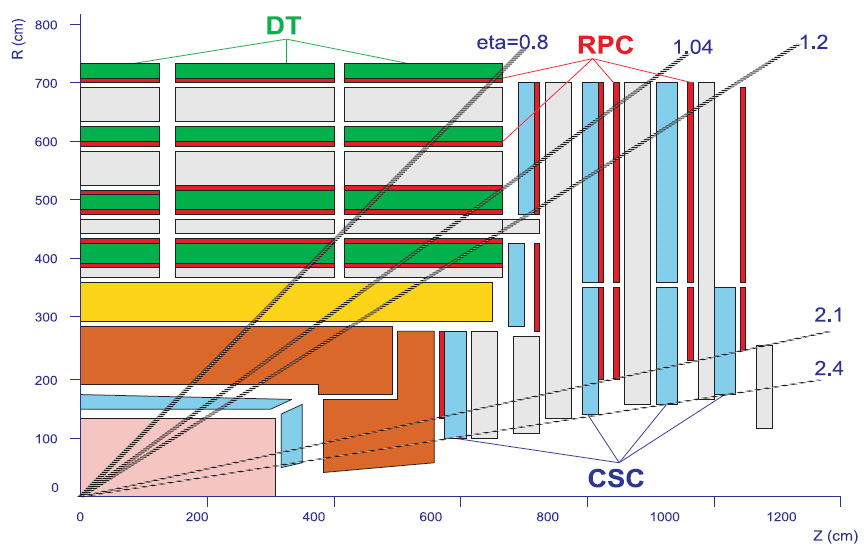
\includegraphics[width=0.7\columnwidth]{bilder/myonsystem.png}%
\caption{Das Myonsystem bei CMS \cite{James:MuonID}.}%
\label{fig:myon}%
\end{figure}

\subsection{Das Triggersystem}

Bei Design-Luminosit�t kommt es innerhalb des CMS-Detektors zu $10^{10}$ Wechselwirkungen pro Sekunde. Von diesen k�nnen allerdings nur etwa $10^{2}$ Ereignisse pro Sekunde zur sp�teren Analyse gespeichert werden. Die Zeit zwischen zwei Paketkollisionen betr�gt 25\,ns. Die Datenrate muss also von 40\,MHz auf 100\,Hz verringert werden. Zu diesem Zweck wurden zwei Triggersysteme entwickelt: der hardwarebasierte Level-1-Trigger und der softwarebasierte High-Level-Trigger (HLT), die im Folgenden beschrieben werden.

\subsubsection*{Level-1-Trigger}

Der Level-1-Trigger setzt sich aus einem Myon- und einem Kalorimeter-Trigger zusammen. Er triggert die vier Elektronen, Photonen, Tau-Jets, zentralen Jets und Forward-Jets mit der h�chsten transversalen Energie, die vier Myonen mit dem h�chsten transversalen Impuls sowie den $\eta$- und $\Phi$-Wert dieser Objekte mit reduzierter Granularit�t und Aufl�sung des Detektors. Diese Objekte werden dann dem HLT als Startwert �bergeben, wenn der \protect\linebreak{Level-1}-Trigger entscheidet, das Ereignis vollst�ndig auszulesen. F�r diese Entscheidung wird etwa 1\,$\mu$s ben�tigt. W�hrenddessen werden die gesamten Detektorinformationen f�r 3,2\,$\mu$s in einem Puffer zwischengespeichert. Die dem HLT �bergebene Eventrate liegt im kHz-Bereich.

\subsubsection*{High-Level-Trigger (HLT)}

Der softwarebasierte HLT arbeitet mit komplexeren Algorithmen und nutzt die komplette Detektorinformation zur Entscheidung und Berechnung von interessanten Objekten, wie z.B. einem hochenergetischen Myon. Als Startwerte des Rekonstruktionsalgorithmus werden die oben beschriebenen Objekte des Level-1-Triggers benutzt. Dieser Algorithmus ist zwar gegen�ber denen des Level-1-Triggers komplexer, im Vergleich zur sp�teren Nachprozessierung der Daten aber vereinfacht, da man immer noch mit einer sehr hohen Datenrate arbeitet. Der Entscheidungsprozess wird in mehrere Abschnitte unterteilt, die jeweils zus�tzliche Informationen heranziehen. Nach jedem Abschnitt k�nnen Ereignisse verworfen werden. Dies spart Zeit, da nicht die gesamte Detektorinformation einbezogen werden muss. Der HLT ist also effektiv in einen N-Level-Trigger unterteilt. \\
Die Softwareumgebung des Triggers ist dieselbe, die auch f�r die Ereignisgeneration, die Detektorsimulation und die nachfolgende Analyse benutzt wird.

%
%
% Kapitel Theorie
%
%


\chapter{Theoretische Grundlagen}

\section{Das Standardmodell der Teilchenphysik}

Das Standardmodell der Teilchenphysik beschreibt die Elementarteilchen, aus denen die Materie aufgebaut ist, als Fermionen sowie die zwischen ihnen wirkenden Kr�fte als Bosonen. In Tabelle \ref{tab:fermionen} ist die Gruppe der Fermionen mit ihren wichtigsten Eigenschaften beschrieben, die aus sechs Leptonen und sechs Quarks besteht. Au�erdem gibt es zu jedem Elementarteilchen noch ein Antiteilchen mit gleicher Masse, Spin und Isospin, jedoch negierten additiven Quantenzahlen.  Die linksh�ndigen Fermionen weisen dabei bez�glich der schwachen Wechselwirkung eine Dublett-, die rechtsh�ndigen eine Singlett-Struktur auf. \\
Die Wechselwirkung zwischen den Fermionen wird im Standardmodell der Teilchenphysik �ber den Austausch von Eichbosonen mit ganzzahligem Spin. Diese Bosonen stellen die Quantisierungen der entsprechenden Felder dar: das Photon $\gamma$ der elektromagnetischen Wechselwirkung, die W$^{\pm}$- sowie Z$^0$-Bosonen der schwachen Wechselwirkung, sowie acht Gluonen der starken Wechselwirkung. Die jeweiligen Prozesse werden durch die Quanten\-elektrodynamik und die Quantenchromodynamik theoretisch beschrieben, f�r eine tiefer gehende Erl�uterung siehe \cite{Berger:Teilchen}. \\
Eine spezielle Position nimmt das Higgs-Boson im Standardmodell ein. Es tr�gt als einziges Teilchen den Spin 0 und verleiht den schwachen Eichbosonen W$^{\pm}$ und Z$^0$ ihre Masse. Die CMS- \cite{CMS:Higgs} und ATLAS-Experimente \cite{ATLAS:Higgs} am LHC pr�sentierten am 4. Juli 2012 die Entdeckung eines Higgs-artigen, neuen Teilchens mit einer Masse von 125\,GeV.

\section{Das Top-Quark am LHC}

Das Top-Quark wurde 1973 von M. Kobayashi und T. Maskawa \cite{Koba:CPV} postuliert, um die CP-Verletzung im Kaonenzerfall zu erkl�ren und 1995 als letztes Fermion experimentell durch das CDF-Experiment \cite{CDF:Top} sowie das D\O-Experiment \cite{D0:Top} nachgewiesen. Der aktuell beste Messwert der Topmasse,
\nopagebreak
\begin{equation}
m_t = 173,3 \pm 0,5\,(stat.) \pm 1,3\,(syst.)\,\text{GeV}\ ,
\end{equation}
beruht auf der Auswertung von $4.9$\,fb$^{-1}$ Daten, die im Jahre 2011 am LHC gesammelt wurden \cite{PAS:TopMass}. Das Top-Quark ist damit das schwerste Fermion.

\begin{table}[h]%
\caption{Die drei Teilchenfamilien von Quarks und Leptonen mit ihren Quantenzahlen. $Q$ bezeichnet die elektrische Ladung in Einheiten der Elementarladung, $T_3$ die dritte Komponente des schwachen Isospins, $Y$ die Hyperladung \cite{Kuessel:Diplom}.}
\vspace{0.3 cm}
\centering
\begin{tabular}{|c||c|c|c|c|c|c|c|}
\hline
 & 1 & 2 & 3 & $Q\,[e]$ & $T_{3}$ & $Y$ & Farbe \\
\hline
\hline
\multirow{2}{*}{Quarks} & \multirow{2}{*}{ $ \left( \begin{array}{cc}
u  \\ d  \\ \end{array} \right)_{L} $} & \multirow{2}{*}{ $ \left( \begin{array}{cc}
c  \\ s  \\ \end{array} \right)_{L} $} & \multirow{2}{*}{ $ \left( \begin{array}{cc}
t  \\ b  \\ \end{array} \right)_{L} $} & 2/3 & 1/2 & 1/3 & \textit{rgb} \\
 & & & & -1/3 & -1/2 & 1/3 & \textit{rgb} \\
 & u$_{R}$ & c$_{R}$ & t$_{R}$ & 2/3 & 0 & 4/3 & \textit{rgb} \\
 & d$_{R}$ & s$_{R}$ & b$_{R}$ & -1/3 & 0 & -2/3 & \textit{rgb} \\
\hline
\multirow{2}{*}{Leptonen} & \multirow{2}{*}{ $ \left( \begin{array}{cc}
\nu_e  \\ e^-  \\ \end{array} \right)_{L} $} & \multirow{2}{*}{ $ \left( \begin{array}{cc}
\nu_{\mu}  \\ \mu^-  \\ \end{array} \right)_{L} $} & \multirow{2}{*}{ $ \left( \begin{array}{cc}
\nu_{\tau}  \\ \tau^-  \\ \end{array} \right)_{L} $} & 0 & 1/2 & -1 & - \\
 & & & & -1 & -1/2 & -1 & - \\
 & $\nu_{e,R}$ & $\nu_{\mu,R}$ & $\nu_{\tau,R}$ & 0 & 0 & 0 & - \\
 & e$_{R}^-$ & $\mu_{R}^-$ & $\tau_{R}^-$ & -1 & 0 & -2 & - \\
\hline
\end{tabular}
\label{tab:fermionen}
\end{table}

\subsection{Erzeugung von Top-Quark-Paaren}

Die bei der Toppaarerzeugung durch Proton-Proton-Kollisionen am LHC vorherrschenden Prozesse sind die Quark-Antiquark-Annihilation
\begin{equation}
q(p_1)+\overline{q}(p_2)\rightarrow t(p_3)+\overline{t}(p_4)
\end{equation}
sowie die Gluon-Gluon-Fusion
\begin{equation}
g(p_1)+\overline{g}(p_2)\rightarrow t(p_3)+\overline{t}(p_4)\ .
\end{equation}
Hier bezeichnet $p_i$ die Viererimpulse der jeweiligen Teilchen. Abbildung~\ref{fig:topproduktion} zeigt die Feynman-Graphen niedrigster Ordnung dieser Prozesse. Anhand dieser k�nnen nun die quadrierten Matrixelemente f�r die beiden Produktionsmechanismen berechnet werden.. Diese Matrixelemente sind �ber die Anfangszust�nde gemittelt und �ber die Endzust�nde summiert:
\begin{align}
\left|\overline{\mathcal M}\right|^2 (q\overline{q} \rightarrow t\overline{t)} = &(4\pi \alpha_s)^2\frac{8}{9}\left(2\frac{(p_1\cdot p_3)^2+(p_2\cdot p_3)^2}{(p_1 + p_2)^4}+\frac{m_t^2}{(p_1 + p_2)^2}\right)\ , \\
\left|\overline{\mathcal M}\right|^2 (g\overline{g} \rightarrow t\overline{t)} = &(4\pi \alpha_s)^2\left(\frac{(p_1 + p_2)^4}{24(p_1\cdot p_3)(p_2\cdot p_3)}-\frac{3}{8}\right) \nonumber \\
 &\cdot \left(4\frac{(p_1\cdot p_3)^2 + (p_2\cdot p_3)^2}{(p_1 + p_2)^4} + \frac{4m_t^2}{(p_1 + p_2)^2} - \frac{m_t^4(p_1 + p_2)^4}{(p_1\cdot p_3)^2(p_2\cdot p_3)^2}\right) \ .
\end{align}
Der differentielle Wirkungsquerschnitt auf Partonniveau ergibt sich mit dem Flussfaktor $(2(p_1 + p_2))^{-1}$ und dem Phasenraumelement f�r einen 2\,$\rightarrow$\,2-Prozess zu:
\begin{equation}
d\hat{\sigma} = \frac{1}{2(p_1 + p_2)^2}\frac{\text{d}^3p_3}{(2\pi)^32E_3}\frac{\text{d}^3p_4}{(2\pi)^32E_4}(2\pi)^4\delta^4(p_1 + p_2 - p_3 - p_4)\left|\overline{\mathcal M}\right|^2
\end{equation}
Um den Wirkungsquerschnitt f�r Proton-Proton-Kollisionen zu bestimmen, m�ssen die Partondichtefunktionen $f_i$ ber�cksichtigt werden, welche die im Proton enthaltenen Partonen beschreiben. Damit ergibt sich:
\begin{equation}
d\sigma = \int\limits_0^1 \int\limits_0^1 dx_1dx_2f_1(x_1,Q^2)f_2(x_2,Q^2)d\hat{\sigma} \ .
\end{equation}
Hier bezeichnet $Q^2$ den Energie�bertrag und $x$ den Impulsanteil des entsprechenden Partons am Gesamtimpuls. Die Produktion von Top-Paaren erreicht genau oberhalb der doppelten Top-Masse ihr Maximum. Dies entspricht bei Schwerpunktsenergien, die am LHC erreicht werden, nur einem kleinen Impulsanteil $x$ am Gesamtimpuls des Protons. Die Partondichteverteilung ist abh�ngig von diesem Impulsanteil und liefert f�r kleine $x$-Werte einen gro�en Gluonanteil. Daher werden am LHC Top-Paare �berwiegend �ber Gluonfusion produziert. Der totale Wirkungsquerschnitt f�r die Top-Paar-Produktion unter Ber�cksichtigung von Diagrammen zweiter Ordnung\,(NNLO) bei einer Schwerpunktsenergie von 7\,TeV berechnet sich zu $163_{-10}^{+11}$\,pb \cite{Kidonakis:Cross}. \\
Abbildung \ref{fig:wirkungsquerschnitt} zeigt den Wirkungsquerschnitt verschiedener Prozesse in Abh�ngigkeit von der Schwerpunktsenergie. Man sieht, dass der Top-Wirkungsquerschnitt mit der Schwerpunktsenergie st�rker ansteigt als wichtige Untergrundprozesse wie z.B. Z- oder QCD-Ereignisse, es ergibt sich somit ein deutlicher physikalischer Gewinn.

\begin{figure}
        \centering
        \begin{subfigure}[b]{0.4\textwidth}
                \centering
                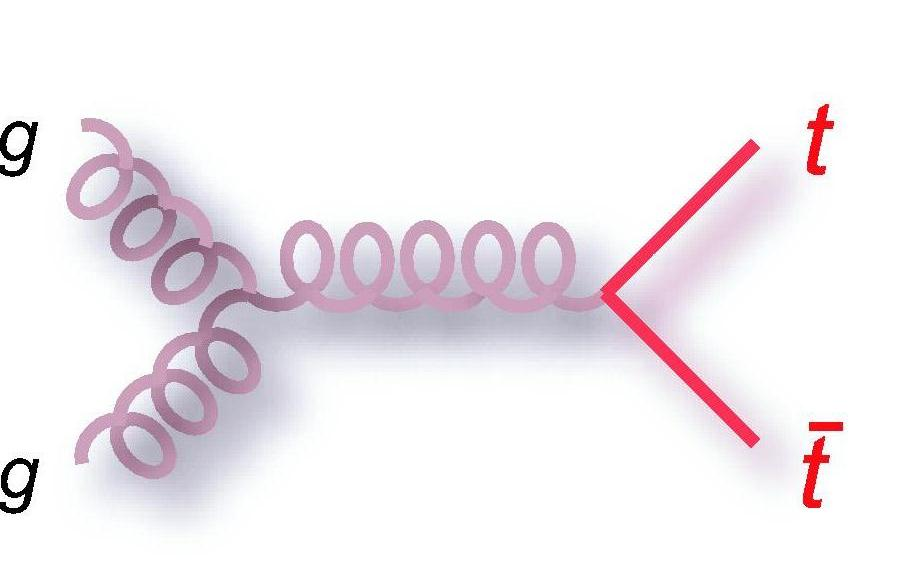
\includegraphics[width=\textwidth]{bilder/gluonfusion-s-kanal}
                \caption{Gluonfusion im s-Kanal}
                \label{fig:gluon-s-kanal}
        \end{subfigure}%
        \begin{subfigure}[b]{0.4\textwidth}
                \centering
                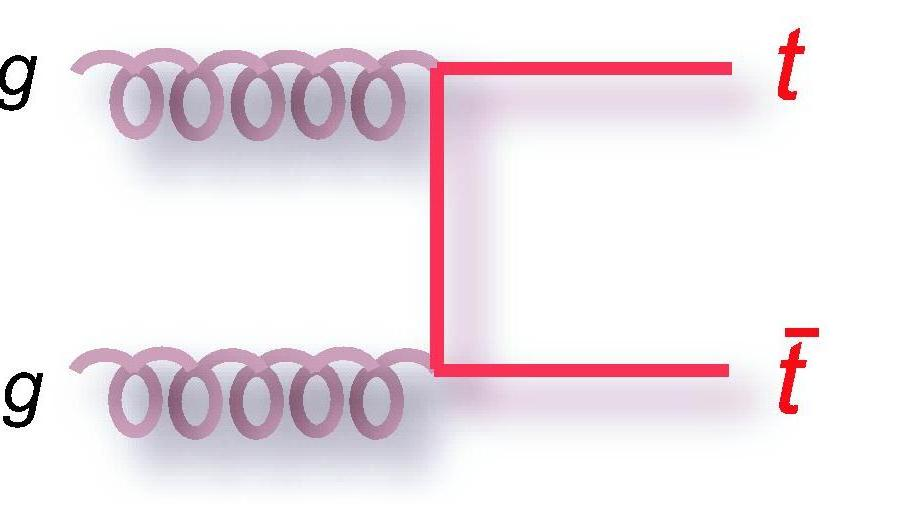
\includegraphics[width=\textwidth]{bilder/gluonfusion-t-kanal}
                \caption{Gluonfusion im t-Kanal}
                \label{fig:gluon-t-kanal}
        \end{subfigure}
        
				\begin{subfigure}[b]{0.4\textwidth}
                \centering
                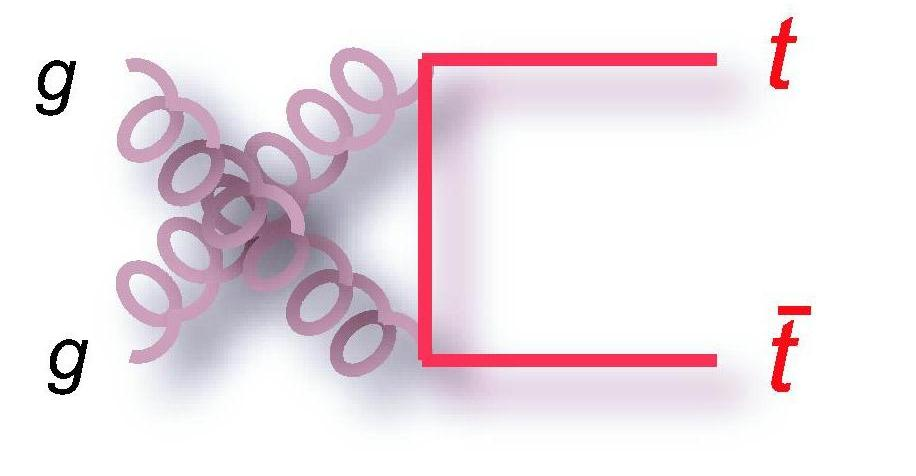
\includegraphics[width=\textwidth]{bilder/gluonfusion-u-kanal}
                \caption{Gluonfusion im u-Kanal}
                \label{fig:gluon-u-kanal}
        \end{subfigure}
				\begin{subfigure}[b]{0.4\textwidth}
                \centering
                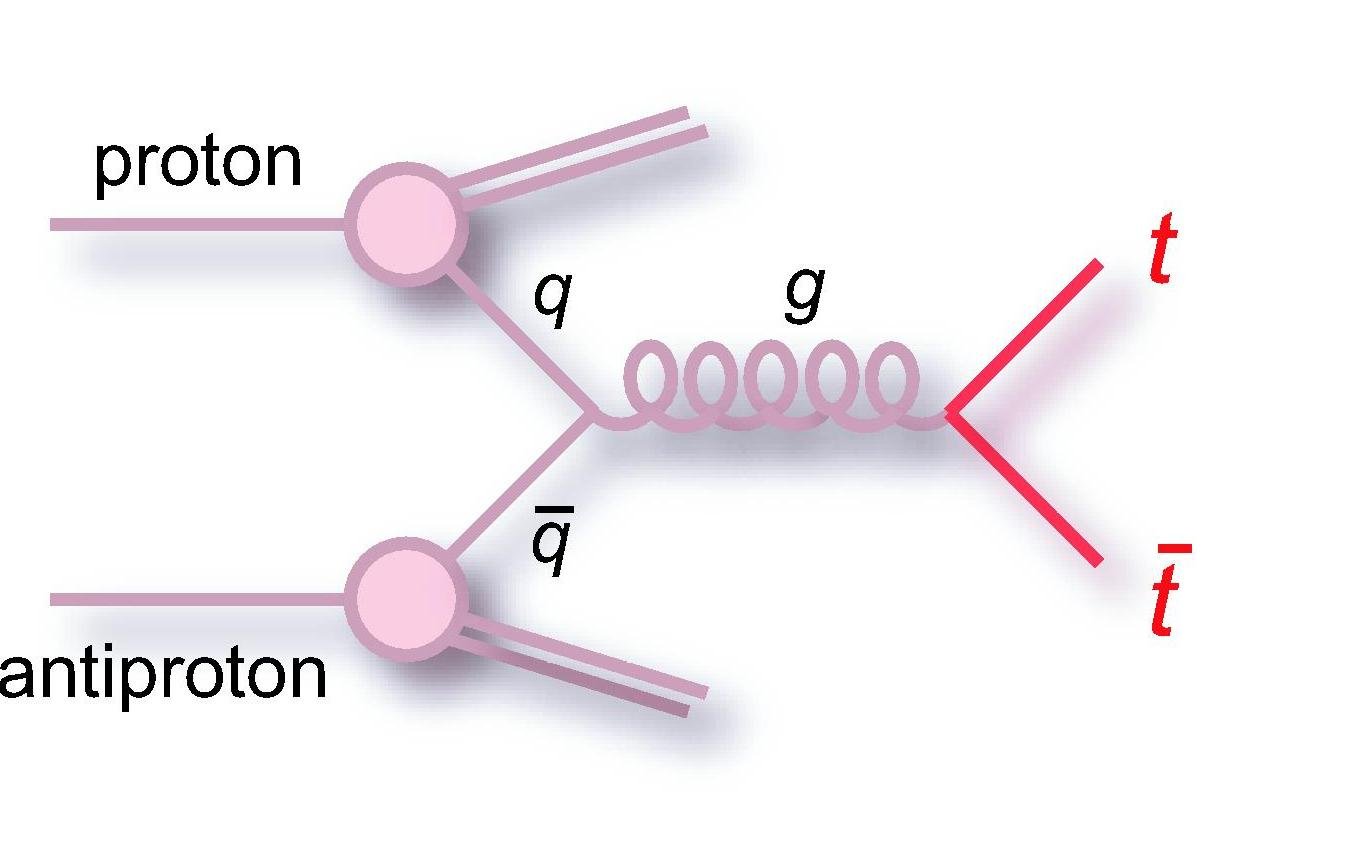
\includegraphics[width=\textwidth]{bilder/quark-annihilation}
                \caption{Quark-Antiquark-Annihilation}
                \label{fig:quark-antiquark}
        \end{subfigure}
				\vspace{0.2 cm}
        \caption{Produktionsmechanismen von Top-Paaren. \cite{Heinson:Diagrams}}\label{fig:topproduktion}
\end{figure}

\begin{figure}%
\centering
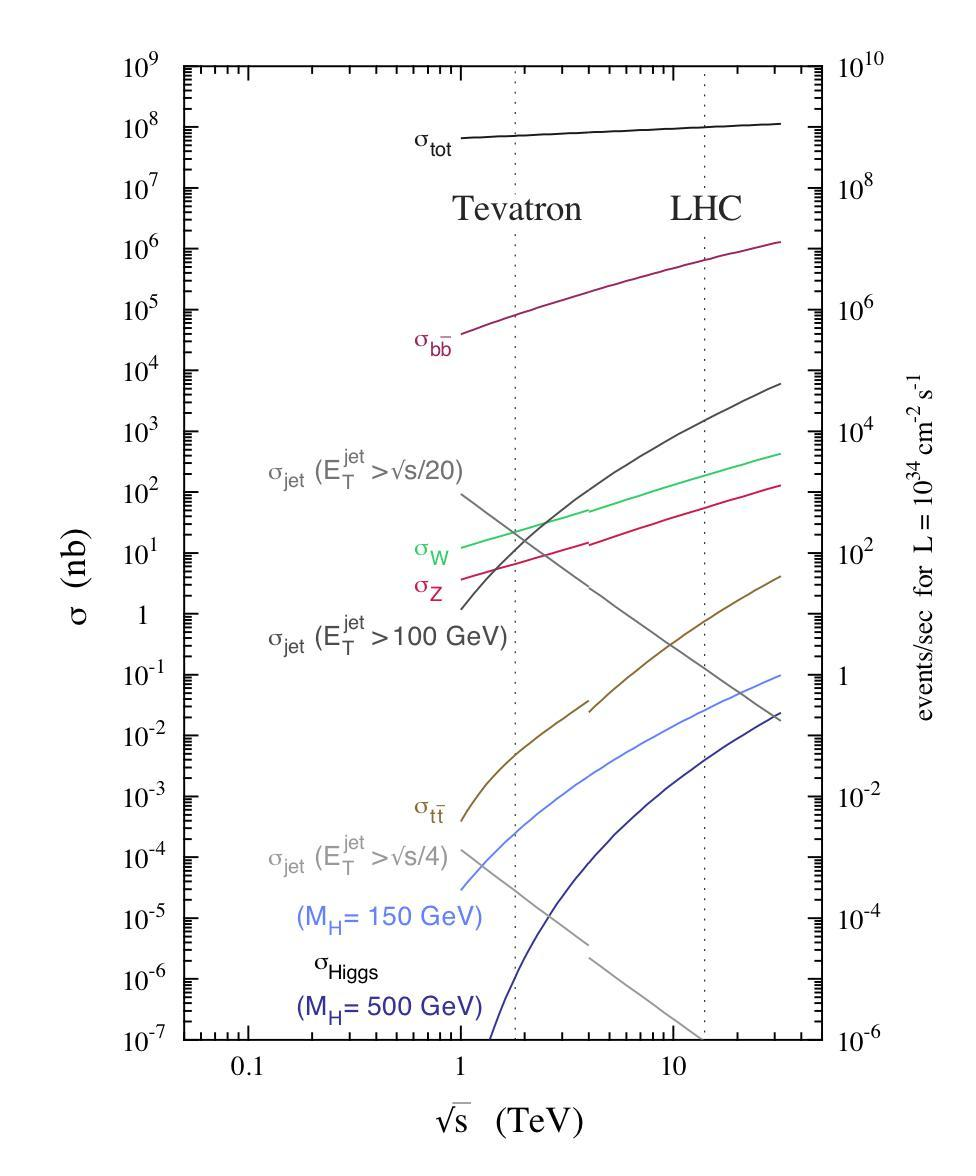
\includegraphics[width=0.8\columnwidth]{bilder/wirkungsquerschnitt}%
\caption{Wirkungsquerschnitte verschiedener Prozesse in Abh�ngigkeit von der Schwerpunktsenergie \cite{Catani:QCD}.}%
\label{fig:wirkungsquerschnitt}%
\end{figure}

\subsection{Top-Quark-Zerfall}

Das Top-Quark zerf�llt �ber die schwache Wechselwirkung fast ausschlie�lich in ein W-Boson und ein b-Quark. Dieser Zerfall wird durch die CKM-Matrix beschrieben
\begin{equation}
B_b = \frac{\left|V_{tb}\right|^2}{\left|V_{tb}\right|^2 + \left|V_{ts}\right|^2 + \left|V_{td}\right|^2} = \left|V_{tb}\right|^2
\end{equation}
unter der Annahme, dass drei Familien von Quarks existieren und damit der Unitarit�t der CKM-Matrix. Vernachl�ssigt man die Masse des b-Quarks und betrachtet nur die niedrigste Ordnung, so ergibt sich f�r die Zerfallsbreite des Top-Quarks
\begin{equation}
\Gamma(t\rightarrow bW) = \frac{G_Fm_t^3}{\sqrt{2}\,8\pi}\left(1 - \frac{m_W^2}{m_t^2}\right)^2 \left(1 + 2\frac{m_W^2}{m_t^2}\right) \ .
\end{equation}
Bei den aktuell gemessenen Top- und W-Massen ergibt sich somit eine Zerfallsbreite des Top-Quarks von $\approx$ 1,4\,GeV und damit eine Lebensdauer von $\tau_{Top} \approx 4,7\cdot 10^{-25}$\,s. Diese liegt deutlich unterhalb der typischen Hadronisationsdauer $\tau_{had} \propto 1/\Lambda_{QCD}$. Top-Quarks bilden deswegen als einzige Quarks keine gebundenen Zust�nde, bevor sie zerfallen. Sie zerfallen direkt und bieten dadurch besondere M�glichkeiten zur Untersuchung des \enquote{freien} Quarkzustandes, insbesondere auch der Kopplungen des Top-Quarks wie in Kapitel~\ref{sec:kopplungen} beschrieben. \\
Die aus dem Zerfall des Top-Quarks entstandenen W-Bosonen zerfallen ihrerseits wiederum im Verh�ltnis, das in Abbildung \ref{fig:verzweigung} gezeigt ist, leptonisch oder hadronisch. In dieser Analyse wird der semimyonische Kanal verwendet, in dem ein W-Boson leptonisch in ein Myon und ein Myonneutrino und das andere hadronisch zerf�llt (siehe auch Kapitel \ref{sec:signatur}). Dieser Kanal stellt einen guten Kompromiss dar. Zum einen verspricht das Verzweigungsverh�ltnis von rund 15\% ein gr��eres Ma� an Statistik als der dileptonische Kanal, zum anderen ist das Signal mit einem Myon gerade im daf�r ausgelegten CMS-Detektor sehr gut zu identifizieren und l�sst sich sehr viel besser vom QCD-Untergrund mit vielen Jets unterscheiden als der vollhadronische Kanal.

\begin{figure}%
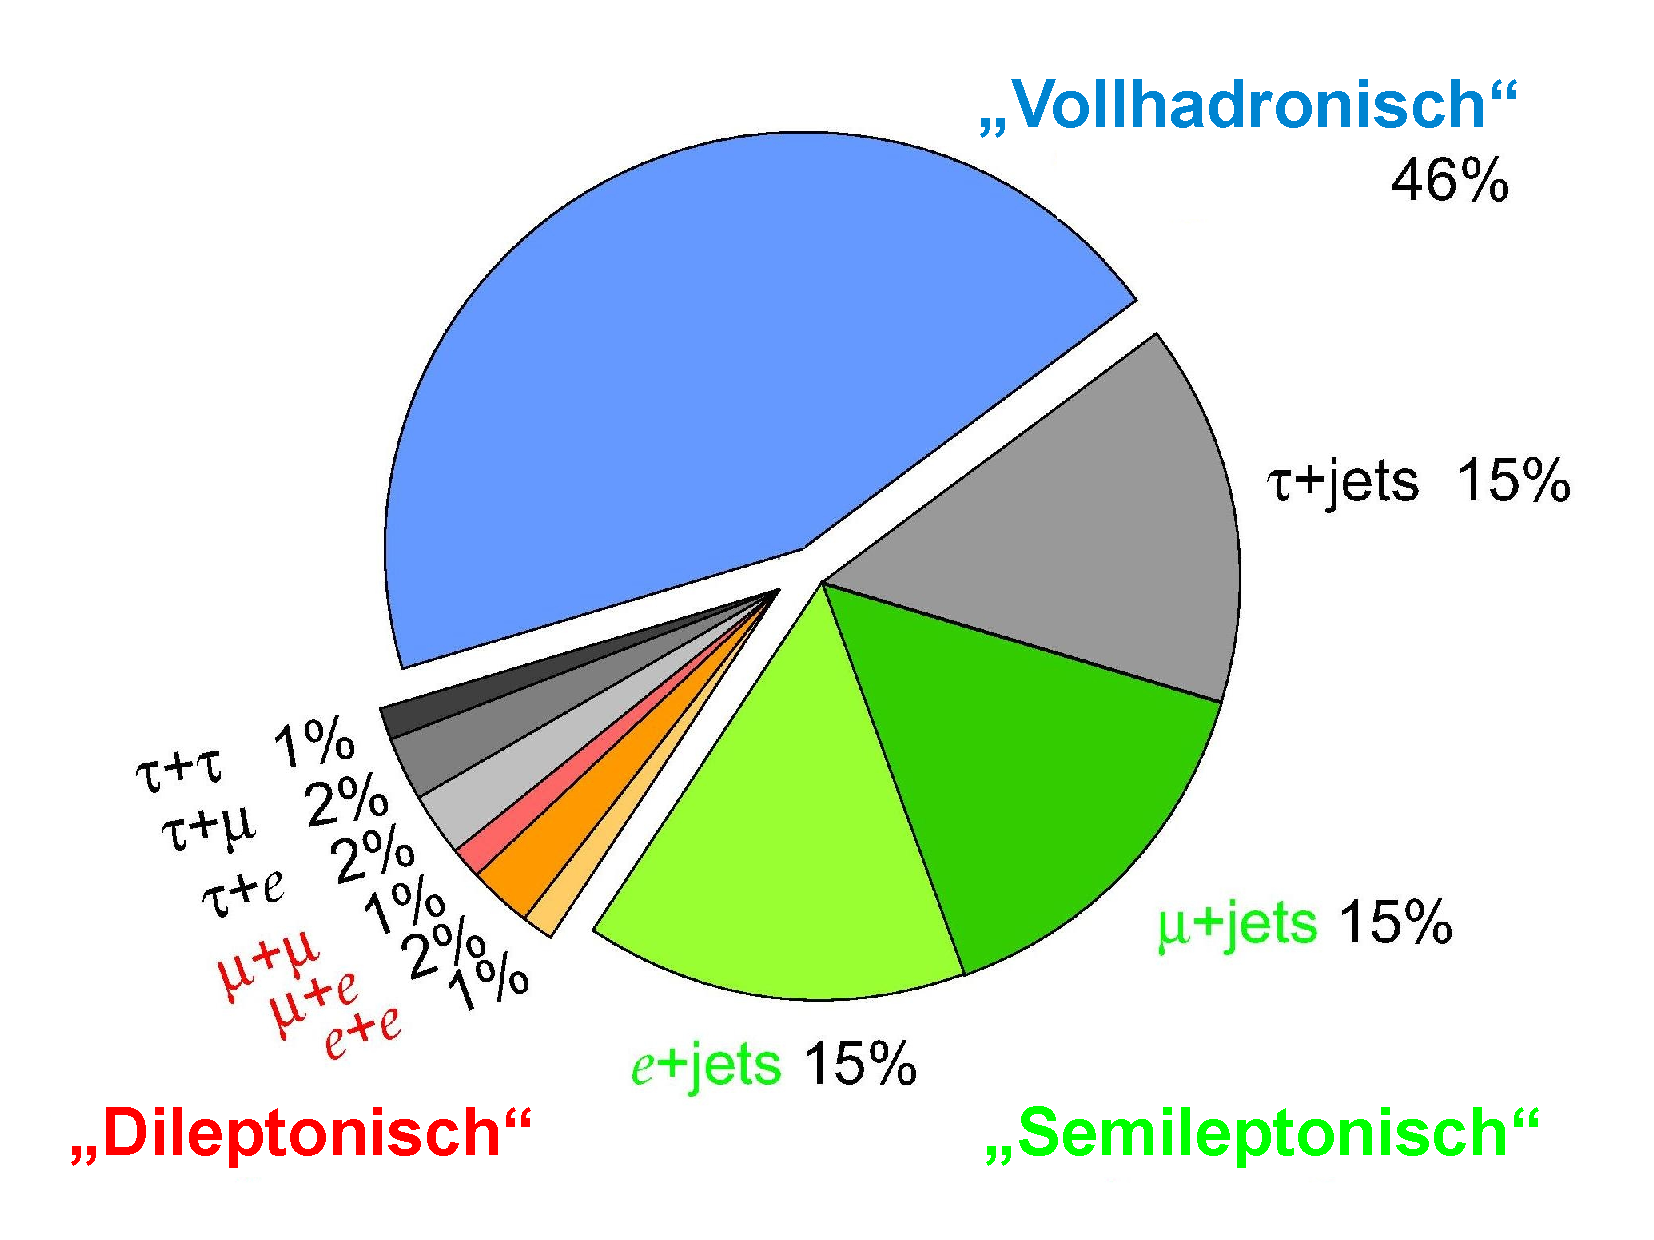
\includegraphics[width=0.9\columnwidth]{bilder/kuchen.pdf}%
\caption{Verzweigungsverh�ltnis der verschiedenen Zerfallskan�le von Top-Paaren \cite{Heinson:Diagrams}.}%
\label{fig:verzweigung}%
\end{figure}

\section{Anomale Kopplungen des Top-Quarks}
\label{sec:kopplungen}

Wie oben beschrieben erlaubt das Top-Quark eine direkte Untersuchung des Quark-Photon-Vertex und dessen Kopplungen. Abweichungen von Standardmodell-Vorhersagen w�rden auf eine anomale Struktur dieses Vertizes hindeuten und somit auch auf Physik jenseits des Standardmodells. \\
Die Kopplungen der Quarks k�nnen bis zu einer Skala $\Lambda$ durch einen Satz von Operatoren $O_x$, sogenannten effektiven Operatoren, parametrisiert werden \cite{Aguilar:Couplings}. Diese sind in einer Lagrangedichte enthalten, welche die Form einer Taylorentwicklung mit komplexen Koeffizienten $C_x$ besitzt:
\begin{equation}
\mathcal L^{\text{eff}} = \sum\frac{C_x}{\Lambda^2}O_x + \cdots
\end{equation}
\begin{figure}%
        \centering
        \begin{subfigure}[b]{0.4\textwidth}
                \centering
                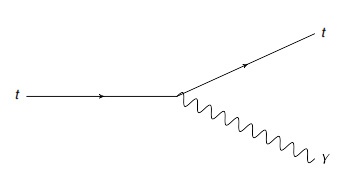
\includegraphics[width=\textwidth]{bilder/vertex1}
                \caption{Feynman-Graph in f�hrender Ordnung (LO).}
                \label{fig:lo-vertex}
        \end{subfigure}%
				\hspace{0.1\textwidth}
        \begin{subfigure}[b]{0.4\textwidth}
                \centering
                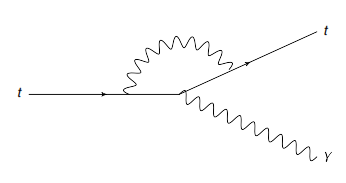
\includegraphics[width=\textwidth]{bilder/vertex2}
                \caption{Mit einer Schleifenkorrektur (NLO).}
                \label{fig:nlo-vertex}
        \end{subfigure}
\caption{Der Top-Photon-Vertex \cite{Tholen:Master}.}%
\label{fig:top-photon-vertex}%
\end{figure}
Der Top-Photon-Vertex ist in Abbildung \ref{fig:top-photon-vertex} dargestellt. Dessen Lagrangedichte ergibt sich zu \cite{Aguilar:Couplings}
\begin{equation}
\mathcal L_{\gamma tt} = -eQ_t\overline{t}\gamma^{\mu}tA_{\mu} - e\overline{t}\frac{i\sigma^{\mu \nu}q_{\nu}}{m_t}(d_V^{\gamma} + id_A^{\gamma}\gamma_5)tA_{\mu}\ .
\end{equation}
Der erste Term ist ein reiner Standardmodell-Beitrag und h�ngt linear von der elektrischen Ladung $Q_t$ des Top-Quarks ab. Damit ist der $t\overline{t} + \gamma$ Wirkungsquerschnitt proportional zu $Q_t^2$. Im zweiten Term entsprechen die Vektor- und Axial-Vektor-Formfaktoren $d_V^{\gamma}$ und $d_A^{\gamma}$ Beitr�ge von Schleifenkorrekturen erster Ordnung, sie beschreiben das magnetische bzw. elektrische Dipolmoment des Top-Quarks. Von den oben angesprochenen acht Operatoren $O_x$ beinhalten $d_V^{\gamma}$ und $d_A^{\gamma}$ die Operatoren $O_{uB\Phi}^{33}$ und $O_{uW}^{33}$. Sie parametrisieren die Abweichung von der Vorhersage des Standardmodells gem��
\begin{equation}
\delta d_V^{\gamma} = \frac{\sqrt{2}}{e}Re\left[c_WC_{uB\Phi}^{33} + s_WC_{uW}^{33}\right]\frac{vm_t}{\Lambda^2}
\end{equation}
\begin{equation}
\delta d_A^{\gamma} = \frac{\sqrt{2}}{e}Im\left[c_WC_{uB\Phi}^{33} + s_WC_{uW}^{33}\right]\frac{vm_t}{\Lambda^2} \ .
\end{equation}
Sollten $\delta d_V^{\gamma}$ bzw. $\delta d_A^{\gamma}$ von Null verschiedene Werte annehmen, so w�re das ein Indikator f�r Ph�nomene jenseits des Standardmodells. Eine Messung dieser Konstanten ist m�glich �ber die Untersuchung des magnetischen bzw. elektrischen Dipolmoments des Top-Quarks. Das magnetische Dipolmoment ist �ber Spinkorrelationsmessungen zug�nglich, w�hrend das elektrische Dipolmoment am Top-Photon-Vertex untersucht werden kann. Abweichungen vom Standardmodell lassen sich beispielsweise am Energiespektrum des Photons ablesen, hier wird f�r gr��ere Werte von $d_A^{\gamma}$ ein h�rteres Spektrum erwartet, siehe auch Kapitel~\ref{sec:montecarlo}.

%
%
% Kapitel Datensimulation
%
%


\chapter{Datensimulation}

\section{Monte-Carlo-Simulation}

Ein Vergleich der Ergebnisse aus von CMS gemessenen Daten mit Monte-Carlo-Simulationen ist eine gute Methode, die Messergebnisse mit Vorhersagen des Standardmodells zu vergleichen. Ebenso k�nnen so Modelle, die davon abweichen, �berpr�ft werden. Das Ziel der Datensimulation ist es, mithilfe von Zufallsgeneratoren und physikalischer Modelle Pseudodaten zu erzeugen. Diese Pseudodaten liegen dann im selben Datenformat vor, in dem auch die echten Daten zur Verf�gung stehen. Somit k�nnen dieselben Analysen sowohl auf gemessene als auch auf simulierte Daten angewendet werden. In diesem Kapitel wird erl�utert, wie die in dieser Analyse untersuchten simulierten Ereignisse produziert werden.

\subsection{Produktionskette}

Die Simulation der Daten erfolgt in mehreren, aufeinander aufbauenden Schritten. Diese sind im Einzelnen:

\begin{enumerate}
	\item Numerische Integration des Matrixelementes (ME) des harten Prozesses und Berechnung des Wirkungsquerschnittes.
	\item Ereignisgeneration: Partonen und Leptonen im Anfangs- und Endzustand der harten Interaktion werden, unter Beachtung der erwarteten Wahrscheinlichkeiten, zuf�llig erzeugt.
	\item Modellierung von Teilchenschauern: Die Abstrahlung von Gluonen und Photonen aus den Teilchen im Anfangs- und Endzustand wird simuliert.
	\item Hadronisierung: Gruppierung von Quarks zu farbneutralen Hadronen.
	\item Hadronischer Zerfall: Der Zerfall von kurzlebigen Teilchen wird reproduziert.
	\item Underlying Event (UE): Hinzuf�gen von Teilchen im Endzustand, die von Protonr�ckst�nden aus dem harten Prozess entstehen.
	\item Pileup: Eine zuf�llige Anzahl von zus�tzlichen, weichen Proton-Proton-Kollisionen wird erzeugt und dem Ereignis hinzugef�gt.
	\item Detektorsimulation: Die Wechselwirkung der in Schritt 2 bis 7 produzierten Teilchen mit dem Detektormaterial und die Detektorantwort werden simuliert.
\end{enumerate}

\subsection{Simulation von \texorpdfstring{$t\overline{t}+\gamma$}{ttg} Ereignissen}

F�r die Simulation des $t\overline{t}+\gamma$-Signals wurde WHIZARD, ein Leading-Order-Monte-Carlo-Generator, benutzt. Ein Schaubild mit verschiedenen simulierbaren Endzust�nden der Monte-Carlo-Generation ist in Abb.\ref{fig:whizard} gezeigt, auf diese soll hier kurz eingegangen werden:

\begin{description}
  \item[2 $\rightarrow$ 3:] Hier werden nur quantenmechanische Interferenzen aus Photonabstrahlungen von Teilchen im Anfangszustand betrachtet. Die Vorteile dieses Modells sind die geringe CPU-Last, die bei der Berechnung der ME anf�llt und die genaue Zuordnung der Photonen zum Top-Vertex. Es zeigt sich aber, dass die Physik hier nicht korrekt beschrieben wird. \cite{Tholen:Master}
	\item[2 $\rightarrow$ 5:] In diesem Modell ist der Zerfall der Top-Quarks ber�cksichtigt, hier tr�gt nun auch die Photonabstrahlung der W-Bosonen und der b-Quarks zum Signal bei. Es stellt einen guten Kompromiss dar zwischen CPU-Auslastung und korrekter Beschreibung der Natur und wird in dieser Analyse benutzt.
	\item[2 $\rightarrow$ 7:] Hier werden alle Photonabstrahlungen des harten Prozesses ber�cksichtigt und die realen Prozesse am pr�zisesten beschrieben, diese Strategie ist jedoch �beraus CPU-intensiv und wird in dieser Analyse nicht weiter verwendet.
\end{description}

\begin{figure}%
\centering
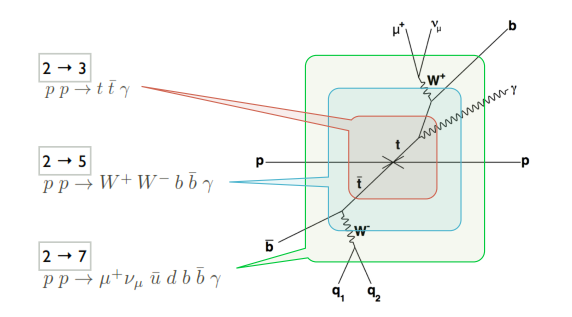
\includegraphics[width=0.7\columnwidth]{bilder/whizard}%
\caption{Strategien der Ereignisgeneration mit WHIZARD. \cite{Tholen:Master}}%
\label{fig:whizard}%
\end{figure}

WHIZARD benutzt die Partondichteverteilung CTEQ6L1 \cite{Pumplin:CTEQ} und eine variable Renorma\-lisierungs- und Faktorisierungsskala. Diese Skalen werden f�r jedes Ereignis auf einen Wert von 172,5\,GeV ($m_t$) plus der Transversalenergie des erzeugten Photons festgelegt. Die Teilchenschauer der Anfangs- und Endzust�nde sowie die Hadronisierung werden von PYTHIA6 \cite{Sjostrand:PYTHIA}, TAUOLA und PHOTOS (beide in \cite{Was:TAUOLA}) simuliert, dabei wird dieselbe Konfiguration wie f�r das Top-Paar-Sample (siehe auch Abschnitt \ref{sec:sim_top_paar} benutzt. \\
An die Teilchen im Endzustand werden bestimmte Anforderungen gestellt, sogenannte \enquote{Produktionsschnitte}. So wird eine minimale transversale Energie gefordert, um Infrarotdivergenz zu vermeiden und eine Minimaldistanz im $\eta-\Phi$-Raum gegen kollineare Divergenz. In dieser Analyse wird eine minimale Transversalenergie des Photons und beider b-Quarks von 10\,GeV und ein $\Delta R > 0,1$ zwischen dem Photon und jedem anderen Teilchen im Endzustand gefordert. Die Messung wird davon nicht beeinflusst, da die Schnitte in der Ereignisselektion noch h�rter sind, siehe Kapitel \ref{sec:selektion}.

\subsection{Simulation des Top-Paar-Prozesses und der betrachteten Untergr�nde}
\label{sec:sim_top_paar}

Die meisten Monte-Carlo-Simulationen neben den $t\overline{t}+\gamma$-Ereignissen werden mit MADGRAPH \cite{Alwall:MADGRAPH} generiert, hier wird die Partondichtefunktion CTEQ6L1 benutzt. Single-Top-Ereignisse werden mit POWHEG \cite{Alioli:POWHEG}, \cite{Re:POWHEG} simuliert, der Zerfall des $\tau$-Leptons mittels TAUOLA. Die Hadronisierung sowie die Teilchenschauer werden mit PYTHIA (hadronische Wechselwirkung) sowie PHOTOS (elektromagnetische Wechselwirkung) modelliert.\
Der Phasenraum der Ereignisse der WHIZARD $t\overline{t}+\gamma$-Simulation ist im MADGRAPH $t\overline{t}$-Sample schon abgedeckt. Deswegen werden Ereignisse aus dem $t\overline{t}$-Sample, welche die Produktionsschnitte in WHIZARD auf Partonebene erf�llen, nicht ber�cksichtigt, um diese �berschneidung zu entfernen.

\subsection{Detektorsimulation}

Der Durchgang der von den Monte-Carlo-Generatoren erzeugten Teilchen durch die einzelnen Detektorkomponenten sowie die dadurch ausgel�sten Signale werden mit dem Programm GEANT4 \cite{Agostinelli:GEANT} modelliert. GEANT4 simuliert anhand der Detektorgeometrie und des Magnetfeldes das Verhalten der einzelnen Teilchen im Detektor. Dabei werden alle elektromagnetischen und hadronischen Wechselwirkungen mit dem Detektormaterial ber�cksichtigt, wie z.B. Schauer in den Kalorimetern. Trifft ein Teilchen aktives Detektormaterial, erzeugt die Simulation das elektrische Signal, welches auch bei einer Messung entstehen w�rde und simuliert die elektronische Auslese der Signale, die Digitalisierung, in den unterschiedlichen Detektorkomponenten. Die Ausgabe der Digitalisierung wird gespeichert und sp�ter in der Rekonstruktion der einzelnen Teilchen verwendet. Diese Rekonstruktion erfolgt mit den gleichen Algorithmen wie die Rekonstruktion experimenteller Daten. Neben der vollst�ndigen Simulation des Detektors (\enquote{FullSim}), die viel Rechenzeit und -aufwand ben�tigt, wurden auch vereinfachte Modelle zur Detektorsimulation entwickelt (\enquote{FastSim}) \cite{CMS:TDR1}. Dadurch werden die Dauer der Simulation und der ben�tigte Speicherplatz erheblich reduziert. Die Daten in dieser Analyse werden mittels FullSim prozessiert.


\section{Studie der von WHIZARD generierten Monte-Carlo-Samples}
\label{sec:montecarlo}

Die Studie der von WHIZARD generierten Monte-Carlo-Daten soll zeigen, wie sich der Wirkungsquerschnitt des $t\overline{t}+\gamma$-Prozesses sowie das $E_T$-Spektrum der Photonen aus dem harten Prozess durch Variation des angenommenen $d_A^{\gamma}$-Wertes ver�ndert. Des weiteren soll untersucht werden, welche Variable sich am besten dazu eignet, zwischen verschiedenen $d_A^{\gamma}$-Szenarien zu unterscheiden. Durch Verwendung von Generatorteilchen werden Aufl�sungseffekte durch die Rekonstruktion sowie Akzeptanzeffekte durch die Selektion vernachl�ssigt.

\subsection{Wirkungsquerschnitt des \texorpdfstring{$t\overline{t}+\gamma$}{ttg}-Prozesses}
\label{sec:wq}

Es wird eine quadratische Abh�ngigkeit des Wirkungsquerschnittes vom Parameter $d_A^{\gamma}$ erwartet, da $d_A^{\gamma}$ linear in das Matrixelement eingeht und der Wirkungsquerschnitt proportional zum Quadrat des Matrixelementes ist. \\
Mit dem Leading-Order-Monte-Carlo-Generator WHIZARD in der Version 2.1.1 werden f�r Werte f�r das elektrische Dipolmoment von $0<d_A^{\gamma}<1$ in Schritten von 0,01 zun�chst die Matrixelemente f�r den harten Prozess generiert. Der Ansatz $2 \rightarrow 5$ wird implementiert mit zwei W-Bosonen, zwei b-Quarks und einem Photon im Endzustand. Die Matrixelement-Berechnung wird so lange fortgef�hrt, bis ein Fehler auf den Wirkungsquerschnitt von unter 1\% errechnet wird. Die so berechneten Wirkungsquerschnitte sind in Abb. \ref{fig:cs_wofit} dargestellt. Eine Anpassung zeigt die erwartete quadratische Abh�ngigkeit. Auff�llig ist der gro�e Fehler auf den Wirkungsquerschnitt bei den Werten $d_A^{\gamma}=0,06$ und $d_A^{\gamma}=0,95$. Dieser l�sst sich auch bei deutlich l�ngerer Berechnung des Matrixelements nicht weiter verringern. Es ist derzeit nicht klar, was diesen gro�en Fehler verursacht. Es wird von einem internen Berechnungsproblem von WHIZARD bei diesen $d_A^{\gamma}$-Werten ausgegangen, da sich die Steuerungsskripte zur Berechnung der verschiedenen Monte-Carlo-Samples ausschlie�lich im vorgegebenen $d_A^{\gamma}$-Wert unterscheiden, ein Fehler in diesen Skripten also auszuschlie�en ist.

\begin{figure}%
\centering
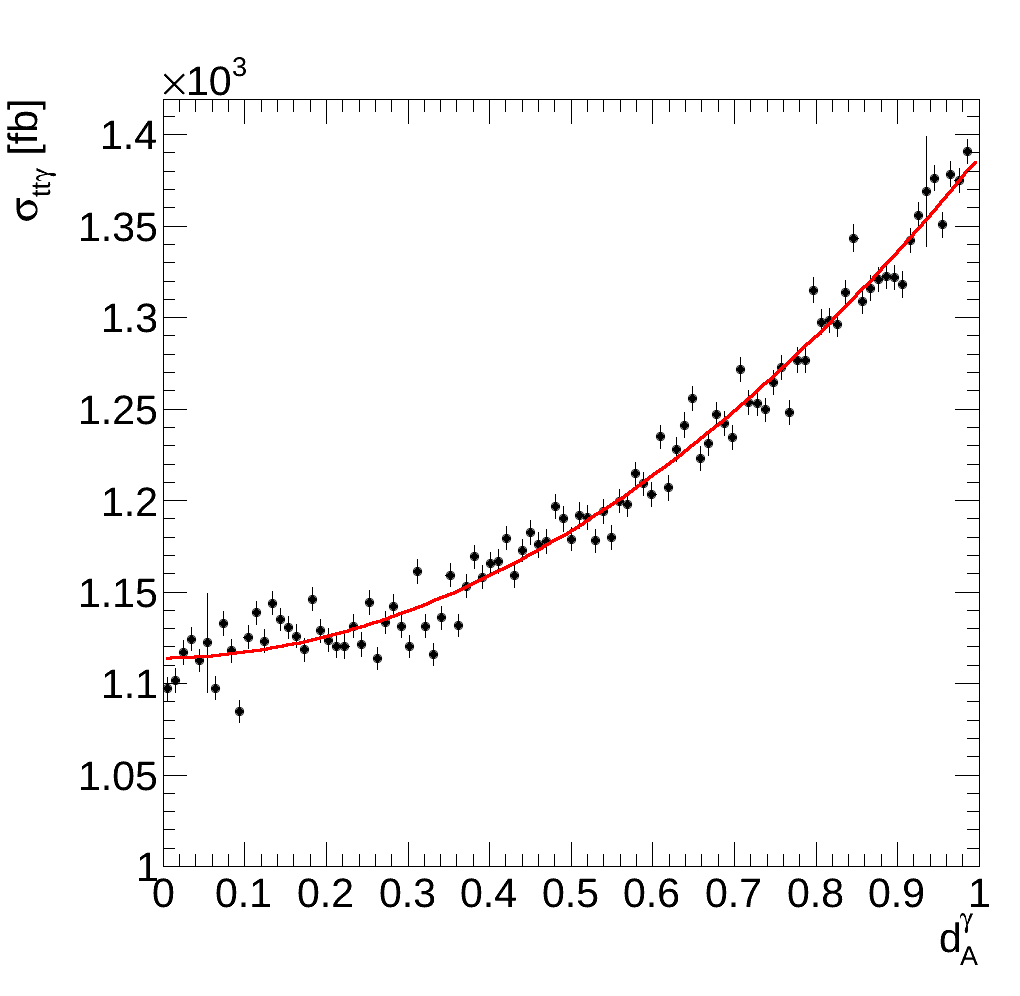
\includegraphics[width=0.5\columnwidth]{bilder/crosssectionplot}%
\caption{Wirkungsquerschnitt des $t\overline{t}+\gamma$-Prozesses f�r $0<d_A^{\gamma}<1$ mit eingezeichneter Fit-Funktion}%
\label{fig:cs_wofit}%
\end{figure}

\subsection{\texorpdfstring{$E_T$}{ET}-Spektrum des Photons}

Aus dem berechneten Matrixelement werden f�r jeden $d_A^{\gamma}$-Wert 105.000 Ereignisse generiert und im Les-Houches-Event Format (LHEF) abgespeichert \cite{Alwall:LesHouches}. Abbildung \ref{fig:et_gen_galerie} zeigt in halblogarithmischer Auftragung ausgew�hlte $E_T$-Spektren dieser generierten Ereignisse. Es best�tigt sich hier die Erwartung, dass sich das Photonspektrum bei einer h�heren Kopplungsst�rke $d_A^{\gamma}$ zu h�heren Energien hin verschiebt. Im folgenden werden mehrere Ans�tze diskutiert, die Abh�ngigkeit des $E_T$-Spektrums von $d_A^{\gamma}$ zu beschreiben.

\begin{figure}%
\begin{subfigure}[b]{0.4\textwidth}
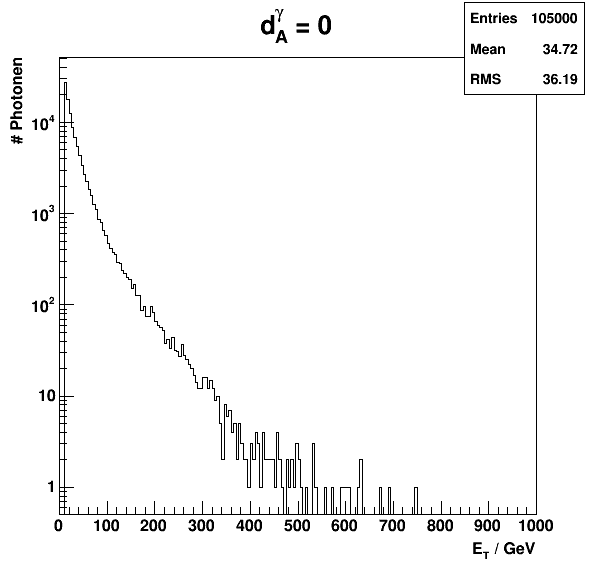
\includegraphics[width=\textwidth]{bilder/et_gen_0}%
\end{subfigure}
\hspace{0.1\textwidth}
\begin{subfigure}[b]{0.4\textwidth}
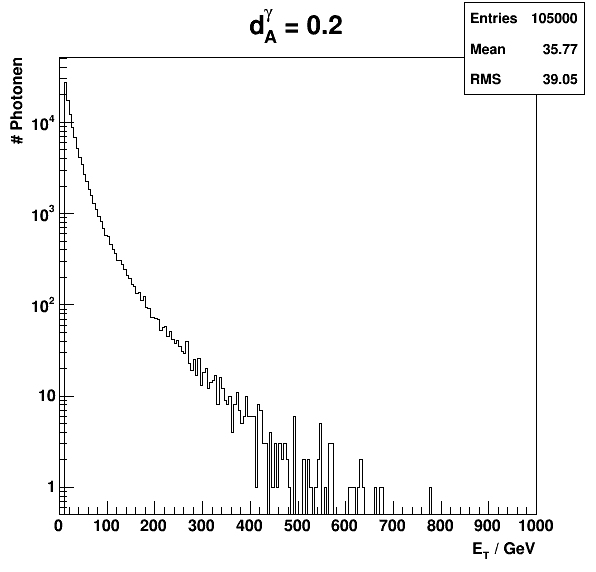
\includegraphics[width=\textwidth]{bilder/et_gen_02}%
\end{subfigure}

\begin{subfigure}[b]{0.4\textwidth}
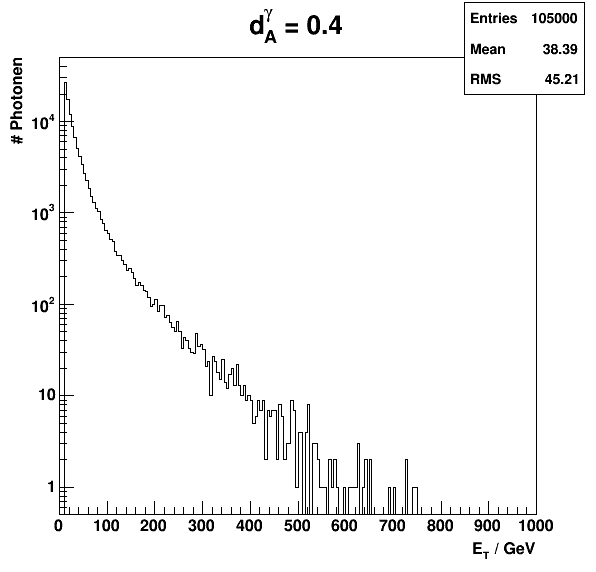
\includegraphics[width=\textwidth]{bilder/et_gen_04}%
\end{subfigure}
\hspace{0.1\textwidth}
\begin{subfigure}[b]{0.4\textwidth}
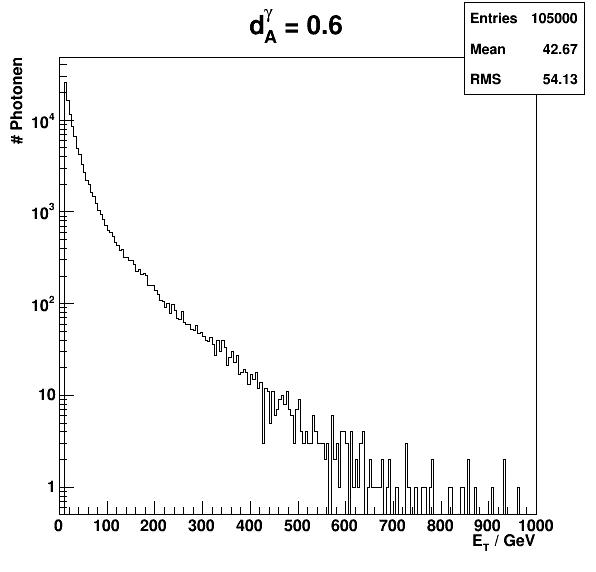
\includegraphics[width=\textwidth]{bilder/et_gen_06}%
\end{subfigure}

\begin{subfigure}[b]{0.4\textwidth}
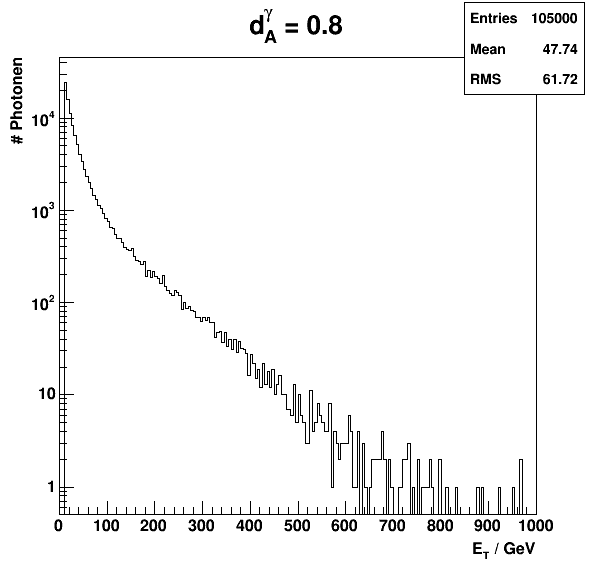
\includegraphics[width=\textwidth]{bilder/et_gen_08}%
\end{subfigure}
\hspace{0.1\textwidth}
\begin{subfigure}[b]{0.4\textwidth}
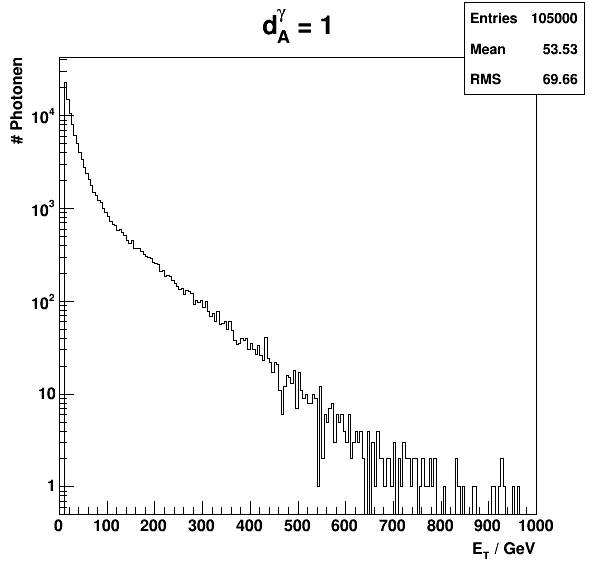
\includegraphics[width=\textwidth]{bilder/et_gen_1}%
\end{subfigure}
\caption{$E_T$-Verteilungen von Monte-Carlo-Daten auf Generator-Level f�r verschiedene Werte von $d_A^{\gamma}$.}%
\label{fig:et_gen_galerie}%
\end{figure}

\subsubsection{2-Bin-Analyse}

Das $E_T$-Spektrum wird in zwei Bereiche aufgeteilt. Der erste Bereich reicht von 0\,GeV bis 100\,GeV, der zweite von 100\,GeV bis 700\,GeV, siehe dazu Abb. \ref{fig:2bin_skizze}. Nun wird das Verh�ltnis der Anzahl der Photonen in den beiden Bereichen gegen $d_A^{\gamma}$ aufgetragen, siehe Abb. \ref{fig:2bin_plot}. Auf der linken Seite sieht man zwei Messwerte, die nicht dem allgemeinen Verlauf folgen. Dies sind die schon in Kapitel \ref{sec:wq} angesprochenen Messpunkte, die durch irreduzibel gro�e Fehler auf den Wirkungsquerschnitt auffielen und auch in allen anderen Analysemethoden herausstechen. Die Punkte $d_A^{\gamma}=0,06$ und $d_A^{\gamma}=0,95$ werden im folgenden f�r die Auswertung der verschiedenen Analysemethoden nicht ber�cksichtigt. Der so bereinigte Plot ist in Abb. \ref{fig:2bin_plot} rechts zu sehen. Die 2-Bin-Analyse stellt einen vielversprechenden Ansatz dar, das h�rtere Photonenspektrum f�r gr��ere Kopplungsst�rken $d_A^{\gamma}$ zu beschreiben. Auf Generatorniveau ist eine sehr gute Separationskraft vorhanden, der Wertebereich erstreckt sich von $E_{Low} / E_{High} = 3,8$ f�r $d_A^{\gamma} = 0$ bis $E_{Low} / E_{High} = 2,2$ f�r $d_A^{\gamma} = 1$ bei einer Unsicherheit von $\Delta E_{Low} / E_{High} \leq 0,03$. 

\begin{figure}%
\centering
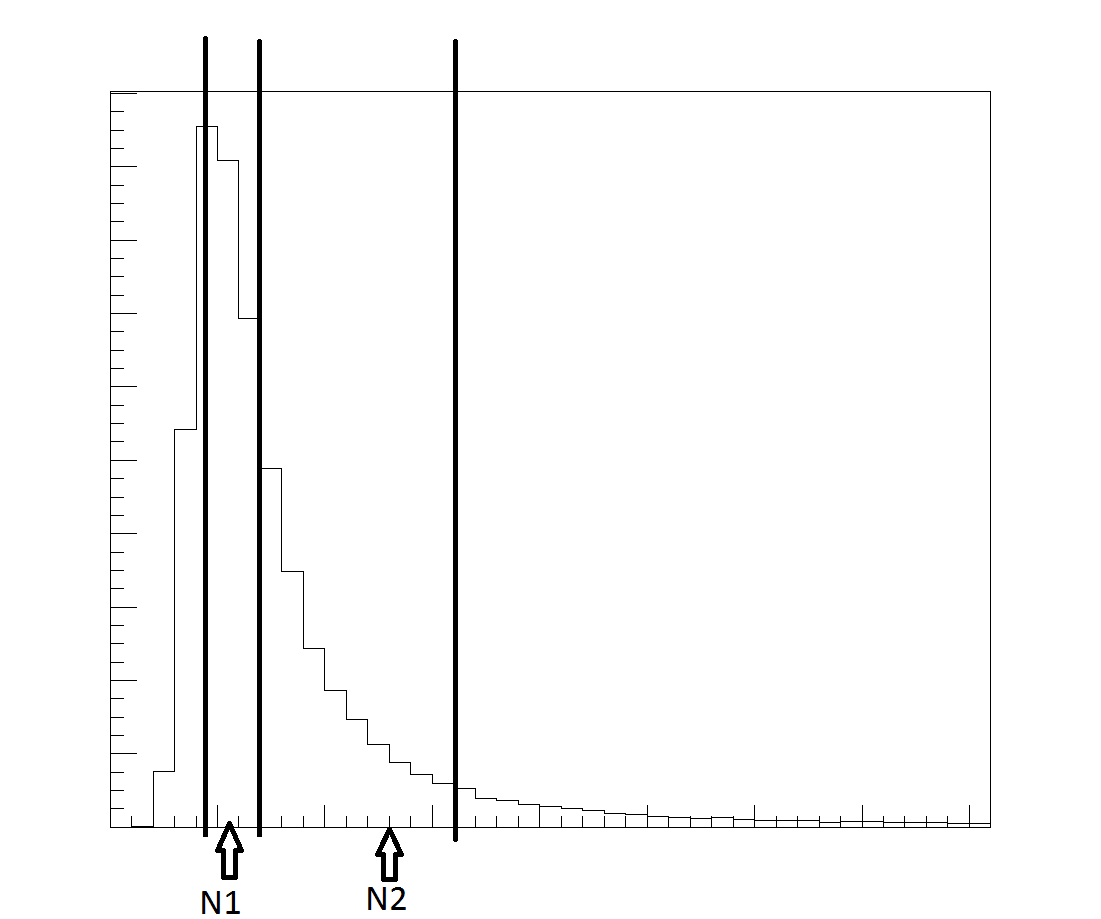
\includegraphics[width=0.5\columnwidth]{bilder/2binskizze}%
\caption{Schema der Unterteilung bei der 2-Bin-Analyse.}%
\label{fig:2bin_skizze}%
\end{figure}

\begin{figure}%
\centering
\begin{subfigure}[b]{0.4\textwidth}
  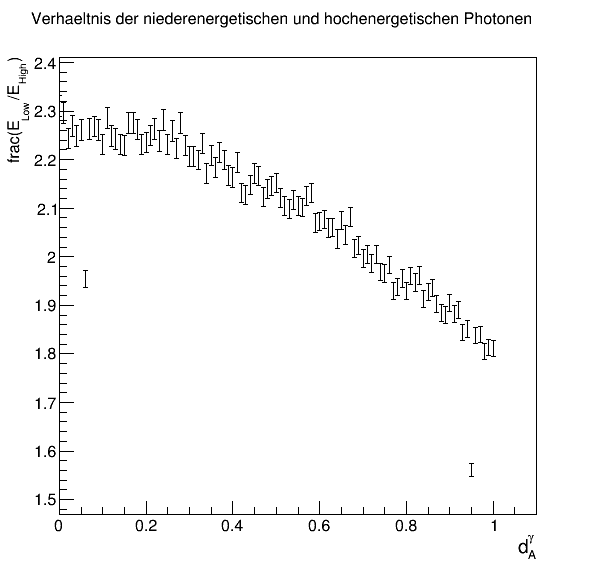
\includegraphics[width=\textwidth]{bilder/twobinplot}%
\end{subfigure}
\hspace{0.1\textwidth}
\begin{subfigure}[b]{0.4\textwidth}
  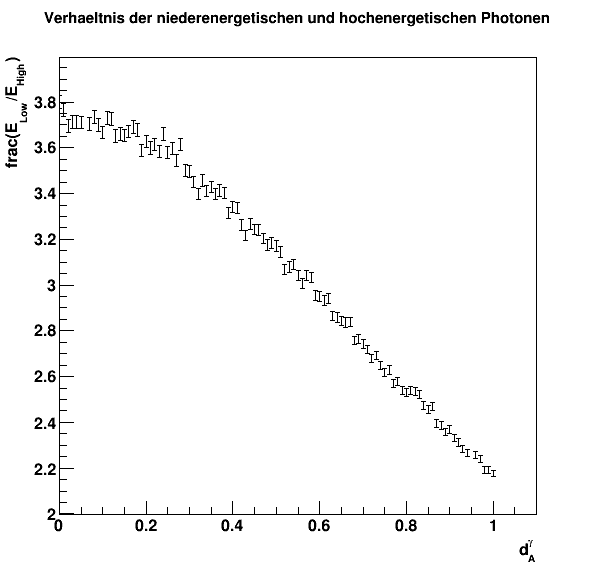
\includegraphics[width=\textwidth]{bilder/twobinplotv2}%
\end{subfigure}
\caption{Verh�ltnis der Anzahl der Photonen in Bin 1 und Bin 2. Im rechten Plot sind die Werte f�r $d_A^{\gamma} = 0,06$ und $d_A^{\gamma} = 0,95$ nicht ber�cksichtigt.}%
\label{fig:2bin_plot}%
\end{figure}

\subsubsection{\texorpdfstring{$E_T$}{ET}-Mean-Analyse}

In diesem Ansatz wird der Schwerpunkt der $E_T$-Verteilung betrachtet, dies ist der gewichtete Mittelwert $\overline{E_T}$ dieser Verteilung. F�r die Berechnung des gewichteten Mittelwertes und des Fehlers auf diesen Mittelwert werden die folgenden Formeln benutzt:

\begin{align}
\overline{E_T} &= \frac{1}{N} \sum{x_i\cdot \omega_i} \\
\Delta \overline{E_T} &= \frac{\sum{(x_i - \overline{E_T})^2 \cdot \omega_i}}{\sqrt{N}} \ .
\end{align}

Hier ist $x_i$ der Mittelpunkt des i-ten Bins des Histogrammes und $\omega_i$ die Anzahl der Eintr�ge in diesem Bin. $E_{T,mean}$ wird gegen $d_A^{\gamma}$ aufgetragen (siehe Abbildung \ref{fig:mean_plot}). Man sieht wiederum eine hohe Separationskraft dieser Variablen auf Generatorniveau, der Wertebereich liegt hier zwischen 34,7 und 53,5\,GeV mit einer Unsicherheit von $\Delta \overline{E_T} \leq 0,22$. 

\begin{figure}%
\centering
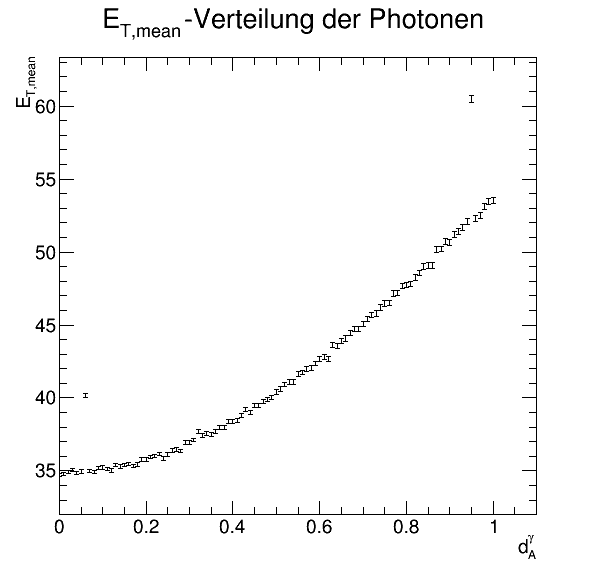
\includegraphics[width=0.5\columnwidth]{bilder/meanplot}%
\caption{Verlauf des Schwerpunktes der $E_T$-Verteilung.}%
\label{fig:mean_plot}%
\end{figure}

\subsubsection{Analyse der Exponentialanpassung der \texorpdfstring{$E_T$}{ET}-Verteilung}
\label{sec:ana_slope}

\begin{figure}%
\centering
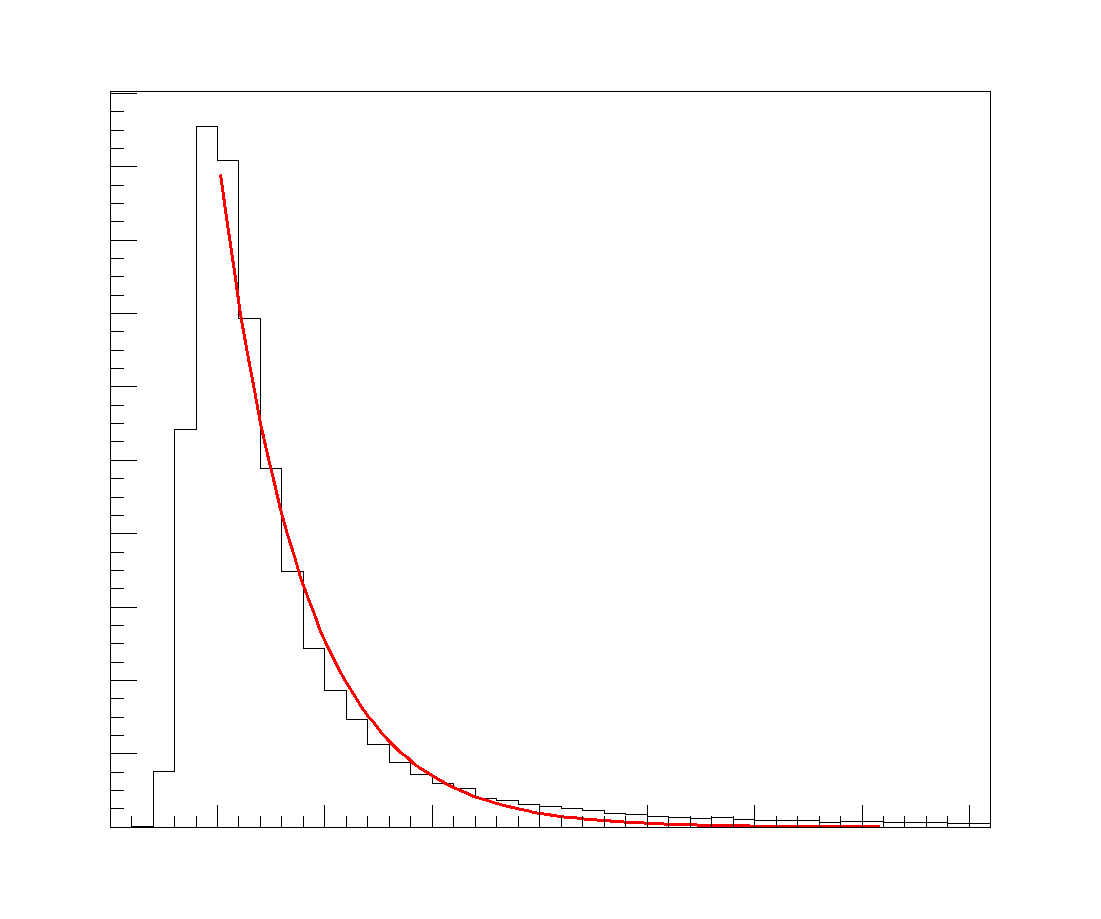
\includegraphics[width=0.5\columnwidth]{bilder/slopeskizze}%
\caption{Skizze zum Prinzip der Exponentialanpassung.}%
\label{fig:slope_skizze}%
\end{figure}

Hier wird die Anpassung einer Exponentialkurve an die $E_T$-Verteilung betrachtet. Wie in Abb. \ref{fig:slope_skizze} zu sehen ist, kann die Verteilung im Bereich zwischen 100\,GeV und 225\,GeV durch eine logarithmische Funktion

\begin{equation}
N(x) = N_0\cdot e^{\lambda \cdot x}
\end{equation}

beschrieben werden. F�r jeden $d_A^{\gamma}$-Wert wird nun an das $E_T$-Spektrum eine Exponentialfunktion angepasst und der Wert von $\lambda$ gegen $d_A^{\gamma}$ aufgetragen. Dieser Plot ist in Abb. \ref{fig:slope_plot} zu sehen. Auch hier ist ein eindeutiger Trend zu erkennen. Die $\lambda$-Werte reichen von -0,0115 bis -0,0218 bei einer Unsicherheit von $\Delta \lambda \leq 0,00053$.

\begin{figure}%
\centering
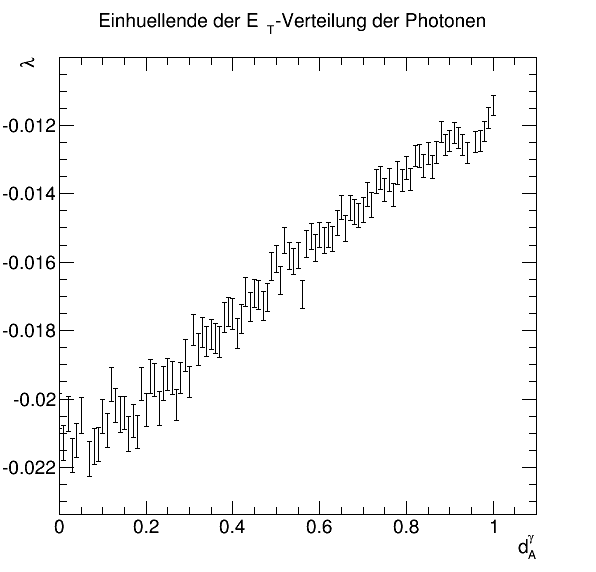
\includegraphics[width=0.5\columnwidth]{bilder/slopeplot}%
\caption{Verlauf des Exponentialkoeffizienten $\lambda$ der Anpassung an die $E_T$-Verteilung.}%
\label{fig:slope_plot}%
\end{figure}

\subsubsection{Vergleich der verschiedenen Analysemethoden}

Alle drei vorgestellten Analysemethoden zeigen auf Generatorniveau eine klare Abh�ngigkeit der untersuchten Variablen von $d_A^{\gamma}$. Dabei weisen die 2-Bin-Analyse sowie die Analyse des Schwerpunktes des Photon-$E_T$-Spektrums die gr��te Separationskraft auf. In der 2-Bin-Analyse liegen zwischen dem Minimal- und dem Maximalwert von $E_{Low}/E_{High}$ rund 50 Standardabweichungen, bei der Analyse von $\overline{E_T}$ sogar 85. Die Analyse der Exponentialanpassung des Photonspektrums weist eine etwas schw�chere Separationskraft auf, hier liegen zwischen den Extremwerten von $\lambda$ 19 Standardabweichungen. \\
Die Unsicherheiten auf die Variablen bei der 2-Bin-Analyse und der Mean-Analyse sind proportional zu $\sqrt{N}$. Es wird demnach f�r die Analyse der selektierten Monte-Carlo-Ereignisse und insbesondere f�r die Analyse von gemessenen Daten eine gr��ere Unsicherheit auf die jeweiligen Variablen erwartet. Bei einer Verringerung von 105.000 Ereignissen (die hier vorgestellte Analyse auf Generatorniveau) auf beispielsweise nur noch 1050 Ereignisse ist die 10-fache Unsicherheit auf die Werte von $E_{Low}/E_{High}$ und $\lambda$ zu erwarten. Wie sehr die Unsicherheit auf die Exponentialanpassung von der Anzahl der untersuchten Ereignisse abh�ngt, ist weitaus schwieriger zu quantifizieren, es wird aber davon ausgegangen, dass die Abh�ngigkeit nicht so stark ist wie bei den anderen beiden Analysen. Des weiteren werden zu den hier besprochenen statistischen Unsicherheiten bei der Rekonstruktion und Selektion auch systematische Unsicherheiten entstehen, welche die Separationskraft der analysierten Variablen weiter abnehmen lassen wird.

%
%
% Kapitel Selektion
%
%


\chapter{Ereignisrekonstruktion und -selektion}

\section{Ereignisrekonstruktion}
\label{sec:reco}

Die Ereignisrekonstruktion erstellt aus den Messwerten der verschiedenen Subdetektoren Kandidaten f�r physikalische Objekte wie z.B. Myonen, Elektronen, Photonen oder Jets und verwendet dazu die digitalisierten Ausgangssignale des Detektors. Abbildung~\ref{fig:reco} zeigt einen Ausschnitt des CMS-Detektors und die unterschiedlichen Signaturen, die beim Teilchendurchgang durch den Detektor erzeugt werden. Als einzige detektierbare Teilchen durchqueren Myonen den gesamten Detektor und hinterlassen Spuren in allen Subdetektoren. Bei hohen Energien dominiert f�r Elektronen der Energieverlust durch Bremsstrahlung. Diese hinterlassen daher nur einen Eintrag im Spurdetektor und werden im elektromagnetischen Kalorimeter gestoppt. Photonen sind elektrisch neutral und hinterlassen somit nur Eintr�ge im elektromagnetischen Kalorimeter. Stark wechselwirkende Teilchen sind in den meisten F�llen geladen und hinterlassen somit auch eine Spur im Spurdetektor, weiterhin deponieren sie Energie im elektromagnetischen und im hadronischen Kalorimeter. \\
Die Rekonstruktion untersucht diese Signaturen, um R�ckschl�sse auf die erzeugten Teilchen zu ziehen. In der CMS Kollaboration werden sogenannte \enquote{Physics Object Groups} (POG) gebildet, die sich auf die Rekonstruktion einzelner Teilchenarten spezialisieren und die Objekte definieren, mit denen in Physik-Analysen gearbeitet wird. Im folgenden wird ein kurzer �berblick gegeben, wie verschiedene Objekte zu Leptonen oder Jets rekonstruiert werden.

\begin{figure}%
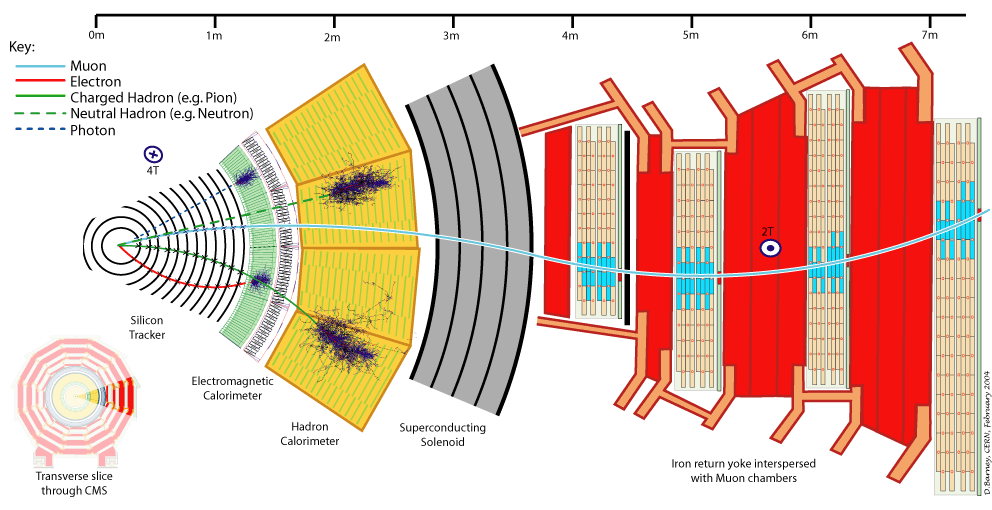
\includegraphics[width=\columnwidth]{bilder/reco}%
\caption{Ein Ausschnitt des CMS Detektors mit Signaturen verschiedener Teilchen \cite{CMS:Slice}}%
\label{fig:reco}%
\end{figure}

\subsection{Myonen}
\label{sec:Reco_Myon}

Myonen k�nnen vom CMS-Detektor konstruktionsbedingt �beraus pr�zise detektiert werden \cite{CMS:TDR1}. Myonen sind geladene Teilchen, ihre Spur ist demnach im Tracker gekr�mmt und sie hinterlassen in jedem weiteren Subdetektor eine spezifische Signatur, die zur Rekonstruktion genutzt werden kann. Ein hochenergetisches Myon verliert in den Kalorimetern nur wenig Energie und erzeugt ab einer Energie von 4\,GeV Eintr�ge im Myonsystem. Die Algorithmen der Rekonstruktionssoftware kombinieren die Informationen des Trackers und des Myonsystems und profitiert so von der speziellen Myon-Signatur. Es wird zwischen \enquote{standalone muons}, die ausschlie�lich anhand von Informationen des Myonsystems rekonstruiert werden, und \enquote{global muons}, die aus der Kombination von Spurdetektor und Myonkammern gebildet werden, unterschieden. \\
Als Startwert f�r die Erzeugung von standalone muons dienen zum einen die Myonen, welche vom L1-Trigger rekonstruiert wurden, zum anderen Regionen erh�hter Aktivit�t im Myonsystem. In den umliegenden Myonkammern wird dann nach charakteristischen Eintr�gen gesucht, die eine Spur bilden k�nnten. Schlie�lich wird ein Kalman-Filter angewendet \cite{Kalman:Filter}. Zun�chst von innen nach au�en, dann von au�en nach innen, wird ein iterativer Fit der Spur in den einzelnen Detektorlagen durchgef�hrt. Die Spurparameter der Ausgangsspur werden dabei in die jeweils n�chste Ebene der Myonkammern projiziert. Wenn das $\chi^2/ndf$ des Fits gr��er ist als ein Maximalwert von 25 oder nicht mindestens zwei Eintr�ge der Anpassung in den Myonkammern verwendet wurden, davon mindestens einer in den Driftkammern oder Kathodenstreifenkammern, wird die Spur verworfen. Als letzte Forderung an die Myonspur wird gestellt, dass sie aus dem Wechselwirkungspunkt stammen muss, der in den Fit mit einbezogen wird. So wird die Impulsaufl�sung des Myons verbessert und gegen kosmische Myonen gefiltert. Die Teilchenspuren in den inneren Spurdetektoren werden auf eine �hnliche Weise mittels eines Kalman-Filters rekonstruiert \cite{Adam:Reco}. Wie im Myonsystem wird hier ausgehend von einem Startpunkt in der n�chsten Detektorlage nach einem Eintrag gesucht, der dann in den Fit einbezogen wird. In den Spurdetektoren finden sich jedoch aufgrund der hohen Teilchenrate mehrere passende Eintr�ge. Diese werden parallel verarbeitet, und nur die besten f�nf Spuren werden nach jedem Schritt nicht verworfen. Als weitere Forderung m�ssen mindestens f�nf Eintr�ge in den einzelnen Lagen des Trackers Verwendung finden. Die so von au�en nach innen rekonstruierte Spur wird auch hier noch einmal in Richtung des Strahlrohres gefittet. \\
Um ein globales Myon zu rekonstruieren, werden Spuren aus dem Myonsystem mit Spuren der inneren Spurdetektoren kombiniert. Dabei geht man von einem bereits rekonstruierten standalone muon aus und nutzt die rekonstruierten Spuren in den Spurkammern. Zun�chst wird abh�ngig von Parametern des standalone muons wie Ort und Impuls ein Raumwinkelbereich definiert, aus dem innere Spuren ber�cksichtigt werden. Dieser Bereich ist rechteckig in der $\eta-\Phi-$Ebene. Dann werden die Tracker-Spuren und die Trajektorie des standalone muons auf eine gemeinsame Fl�che in $\eta$ und $\Phi$ extrapoliert, auf der die Suche nach bester �bereinstimmung vorgenommen wird. Die Wahl dieser Fl�che ist abh�ngig vom Myonimpuls. Auf der gemeinsamen Fl�che werden nun unter Verwendung von �rtlichen Diskriminatoren, die f�r hochenergetische Myonen besonders effektiv sind, sowie Impulsdiskriminatoren, die f�r die Auswahl niederenergetischer Myonen relevant sind, iterativ die besten �bereinstimmungen der Spuren gesucht. Im Allgemeinen bleiben durch diesen Schritt mehrere Tracker-Spuren �brig. Schlie�lich werden alle m�glichen Paare von standalone muons und den ausgew�hlten Tracker-Spuren global gefittet. Bei mehreren m�glichen Paarungen wird die ausgew�hlt, deren Fit das niedrigste $\chi^2/ndf$ aufweist. So wird aus jedem standalone muon maximal ein globales Myon gebildet. \\
In Abbildung~\ref{fig:reco_eff_muon} und \ref{fig:reco_res_muon} ist ein Vergleich der Rekonstruktionseffizienz und der $q/p_T$-Aufl�sung, das ist ein Ma� der Spurqualit�t und -kr�mmung, der \enquote{standalone} mit den globalen Myonen zu sehen. Die Rekonstruktionseffizienzen sind in $\left| \eta \right|$ vergleichbar, die $q/p_T$-Aufl�sung ist f�r globale Myonen um eine Gr��enordnung verbessert. Die verschlechterung der Effizienz in lokalen $\left| \eta \right|$-Bereichen ist durch L�cken zwischen den aktiven Detektorelementen verursacht, in den �brigen Bereichen liegt die Effizienz zwischen 95 und 99\%.

\begin{figure}%
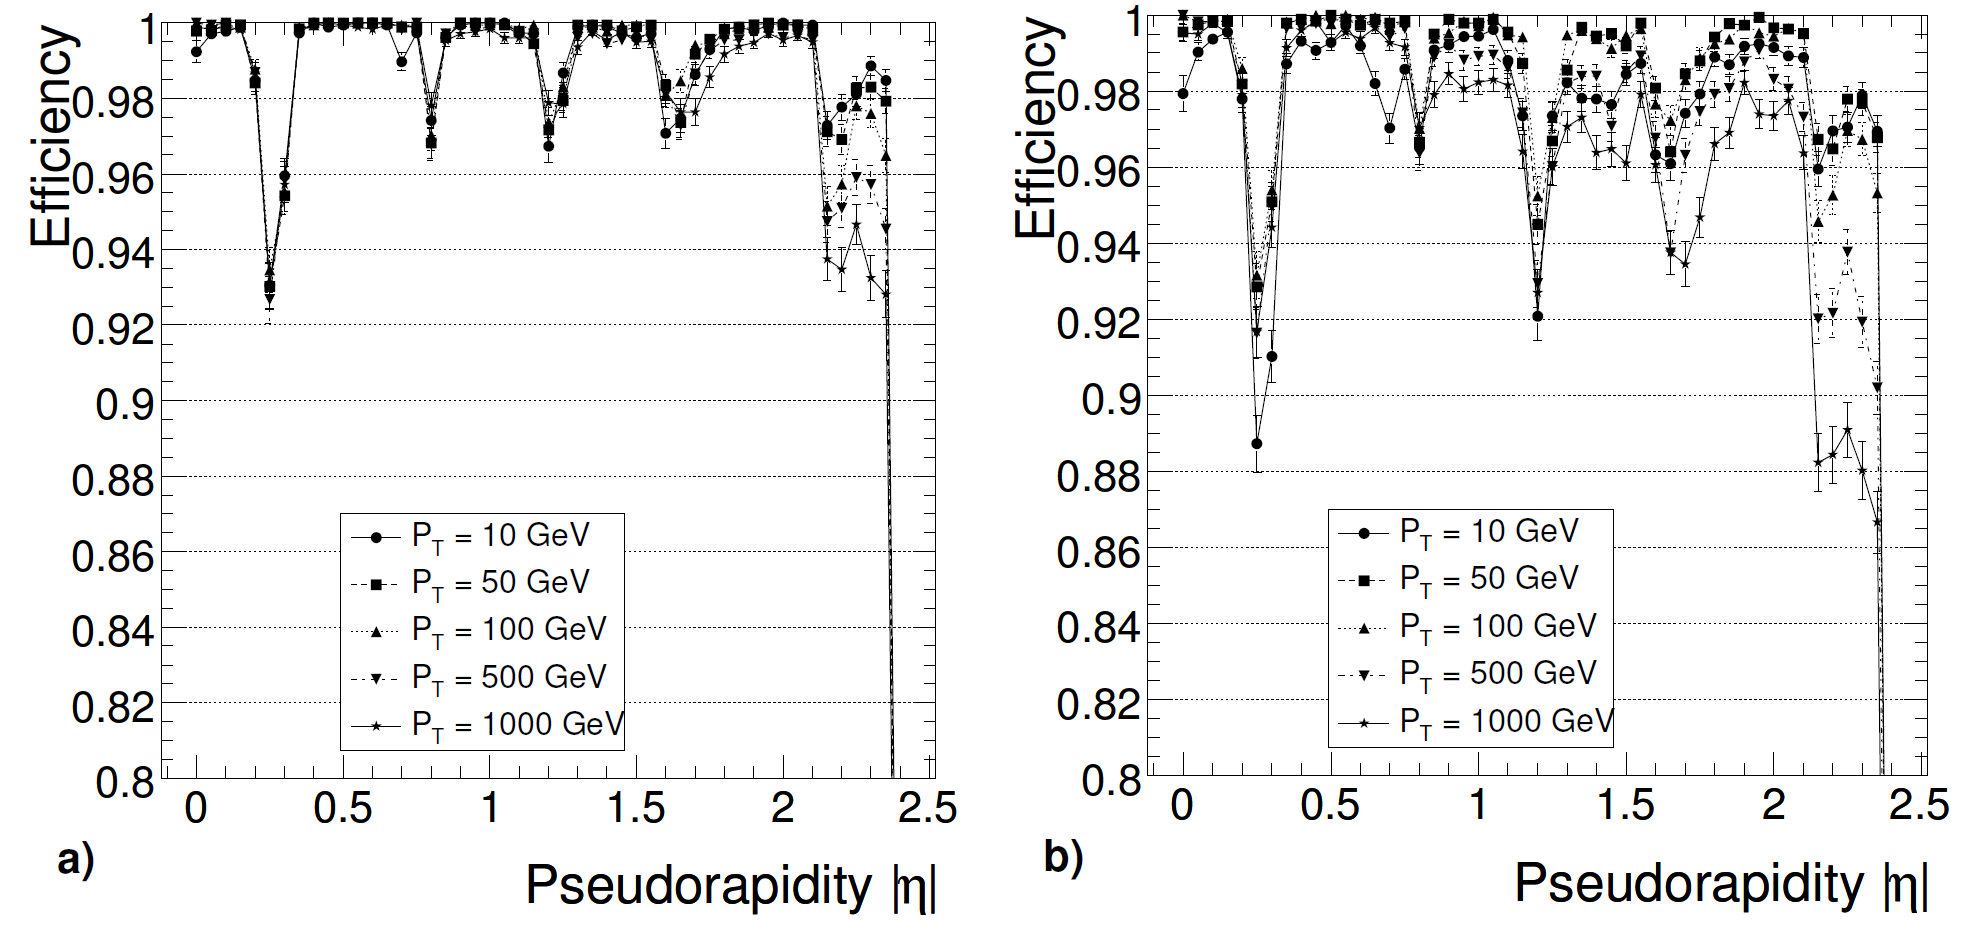
\includegraphics[width=0.9\columnwidth]{bilder/reco_eff_muon}%
\caption{Rekonstruktionseffizienz f�r Myonen als Funktion der Pseudorapidit�t f�r verschiedene $p_T$-Werte. a) \enquote{standalone} Myonen; b) global rekonstruierte Myonen \cite{CMS:TDR1}.}%
\label{fig:reco_eff_muon}%
\end{figure}

\begin{figure}%
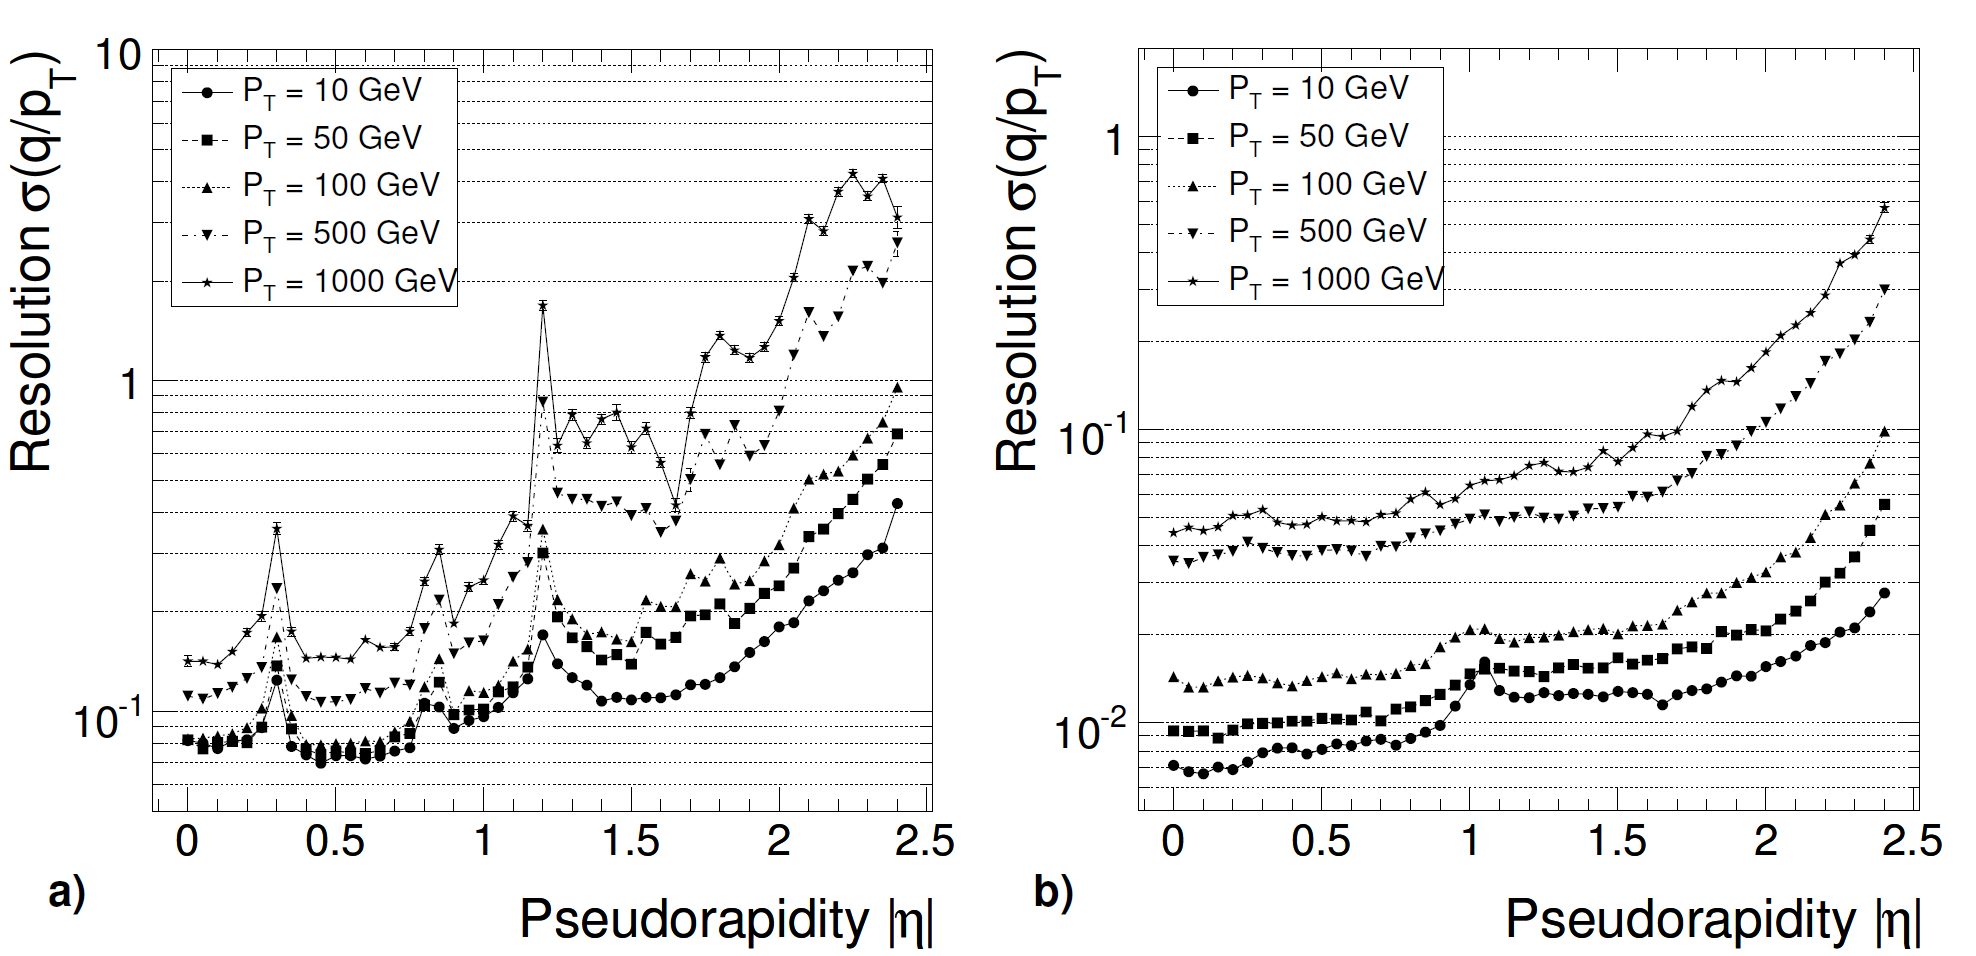
\includegraphics[width=0.9\columnwidth]{bilder/reco_res_muon}%
\caption{$q/p_T$-Aufl�sung f�r a) \enquote{standalone} und b) global rekonstruierte Myonen in Abh�ngigkeit von der Pseudorapidit�t \cite{CMS:TDR1}.}%
\label{fig:reco_res_muon}%
\end{figure}

\subsection{Elektronen}

Das Fehlen einer eindeutigen Signatur, wie sie bei den Myonen durch Eintr�ge in den �u�eren Myonkammern vorhanden ist, erschwert die Rekonstruktion von Elektronen. Elektronen sind ebenso wie Myonen geladene Teilchen und hinterlassen so Spuren in den Silizium-Spurdetektoren, zus�tzlich schauern sie im elektromagnetischen Kalorimeter auf. Somit gibt es zwei M�glichkeiten der Rekonstruktion: entweder von den Eintr�gen im ECAL (\enquote{ECAL-getrieben}) oder von den Spuren im Silizium-Tracker (\enquote{Tracker-getrieben}) ausgehend. Letztere Methode ist nur f�r niederenergetische oder nicht isolierte Elektronen von Bedeutung, daher wird im folgenden der ECAL-getriebene Algorithmus erl�utert \cite{Baffioni:Reco}: \\
Den Ausgangspunkt bilden hier sogenannte \enquote{Supercluster} im ECAL. Diese bestehen aus mehreren Kristallbl�cken, in denen Energie deponiert wurde (\enquote{Cluster}). Mittels verschiedener Algorithmen wird die aufgrund von Bremsstrahlung entlang der $\Phi$-Richtung verteilte Energie zusammengefasst. Energieeintr�ge in einem Bereich von $\Delta \Phi \approx 0,3$\,rad um den Startcluster werden ber�cksichtigt. Die Richtung des urspr�nglichen Elektrons entspricht dem Schwerpunkt des Superclusters, wenn dieser alle durch Bremsstrahlung abgestrahlte Energie enth�lt. Daher wird nach Eintr�gen im entsprechenden $\eta-\Phi-$Bereich in den innersten Lagen des Spurdetektors gesucht, da dort kaum Einfl�sse durch Abstrahlungen zu erwarten sind. Von den so gefundenen Eintr�gen wird von den inneren Spurdetektorlagen ausgehend eine Spur gebildet. Der daf�r genutzte Algorithmus ber�cksichtigt explizite Energieabstrahlungsmodelle f�r Elektronen und unterscheidet sich so vom allgemeinen Spurfit. An jedem Messpunkt werden dazu �berlagerungen von Gau�kurven entsprechend der Vorhersagen der Bethe-Heitler-Formel, die den differentiellen Wirkungsquerschnitt f�r den Energieverlust von Elektronen durch Bremsstrahlung im Feld schwerer Kerne beschreibt \cite{Bethe-Heidler}, verwendet und die Spur mithilfe eines Gau�'schen Summenfilters gefittet \cite{Fruehwirth:Reco}. Die Informationen der gebildeten Elektronenspur wird mit dem Supercluster im ECAL zusammengefasst und dabei eine Reihe von Variablen gespeichert, die sp�ter Informationen �ber die Qualit�t des Elektrons geben k�nnen, darunter z.B. das Verh�ltnis $E/p$. Ambiguit�ten in den Spurdetektoren, die beispielsweise auftreten k�nnen, wenn ein durch Bremsstrahlung erzeugtes Photon durch Paarbildung ein weiteres Elektron erzeugt, welches in diesem Schritt dem urspr�nglichen Elektron zugeordnet werden muss, werden aufgel�st. Dazu wird das urspr�ngliche Elektron durch einen ersten Trackereintrag m�glichst nah am Wechselwirkungspunkt bestimmt. Reicht dieses Kriterium nicht aus, wird das Elektron mit dem gr��eren $E/p$-Verh�ltnis ausgew�hlt. Schlie�lich wird die Ladung der Elektronen bestimmt. Dazu werden drei Methoden benutzt: Ladung der rekonstruierten Elektronenspur, Ladung der n�chsten Spur der normalen Spurrekonstruktion und Vektordifferenz der Vektoren vom Wechselwirkungspunkt zum ersten Siliziumdetektoreintrag und vom Wechselwirkungspunkt zum Supercluster. Die Ladung wird ausgew�hlt, die von mindestens zwei der drei Methoden bestimmt wurde. 

\subsection{Photonen}

Ausgangspunkt f�r die Photonrekonstruktion sind Photon-Kandidaten aus energiekorrigierten Superclustern. Diese Kandidaten m�ssen eine minimale unkorrigierte Energie von mindestens 20\,GeV besitzen und das Verh�ltnis der deponierten Energien in HCAL und ECAL $E_{HCAL}/E_{ECAL}$ muss kleiner als 5\% sein. Ein weiterer Schnitt in $\eta$ wird angewandt, es werden nur Photon-Kandidaten mit $\left|\eta\right|<1,4442$ und $1,566<\left|\eta\right|<2,5$ akzeptiert. Die Richtung des Impulsvektors wird bestimmt, indem der rekonstruierte Prim�rvertex mit der Position des Superclusters, in dem die Energie deponiert wurde, verbunden wird. Die Energie des Photons wird bestimmt aus der korrigierten Energie des Superclusters (konvertiertes Photon) oder der Summe der Energien in einem 5x5 Kristallblock um die h�chste Energiedeposition(Photon aus dem harten Prozess, \enquote{prompt photon}). F�r weitere Details siehe \cite{PAS:Photonreco}. \\
Die hier angesprochenen Photon-Kandidaten sind der Ausgangspunkt f�r die Photonselektion, in welcher weitere Qualit�tsschnitte angewendet werden, um den Anteil der gut rekonstruierten prompt photons zu erh�hen.

\subsection{Geladene und ungeladene Hadronen}

Spuren und Kalorimetereintr�ge, die noch nicht einem Myon, Elektron oder Photon zugeordnet wurden, werden als (geladene oder ungeladene) Hadronen identifiziert und als Funktion von $\eta$ und den Energiedepositionen im ECAL und HCAL rekalibriert.

\subsection{Particle Flow}

Die bisherige Rekonstruktion kann mehrdeutig sein, da viele der Kandidaten denselben Detektoreintr�gen zugeordnet sein k�nnen. Der sogenannte \enquote{Particle Flow}-Algorithmus, der f�r diese Analyse benutzt wird, entfernt diese Ambiguit�t und erstellt eine Liste von exakt rekonstruierten Teilchen. Die Quellen f�r diesen Algorithmus sind Cluster in den Kalorimetern, Spuren aus dem inneren Spurdetektor und voridentifizierte Elektronen und Myonen. Die wesentlichen Schritte des Algorithmus werden im folgenden beschrieben \cite{PAS:Particleflow}:

\begin{itemize}
	\item Im ECAL und HCAL werden sogenannte \enquote{topologische Cluster} aus den urspr�nglichen Clustern gebildet. Die Spuren des inneren Spurdetektors werden zu den Kalorimetern hin extrapoliert.
	\item Eine topologische Verkn�pfung erzeugt sogenannte \enquote{blocks} von wenigen Elementen, dies sind Spuren und Cluster. Die Verkn�pfungen zwischen den Elementen werden nach ihrem Abstand in der $\eta-\Phi-$Ebene bewertet, bei Verkn�pfungen von Eintr�gen im Myonsystem und Spuren im Tracker wird der Wert des $\chi^2$ des globalen Fits als Bewertung verwendet. Bremsstrahlung wird ber�cksichtigt.
	\item Block f�r Block werden alle Mehrdeutigkeiten aufgel�st. Bei mehr als einer M�glichkeit der Aufl�sung von verkn�pften Elementen wird diejenige gew�hlt, welche die beste Bewertung besitzt. F�r jeden Block werden die folgenden Schritte durchgef�hrt:
	\begin{itemize}
		\item Myonen werden mit allen zugeh�rigen Spuren vom Block entfernt. Ein durchschnittlicher Energiebetrag wird von den Kalorimeter-Clustern subtrahiert, dieser Betrag wurde mithilfe von kosmischen Myonen bestimmt.
		\item Die voridentifizierten Elektronen werden noch einmal untersucht, um passende Spuren und Bremsstrahlungsphotonen zu finden. Eine finale Kombination mit Spuren und Kalorimeter-Variablen wird gefittet. Alle damit zusammenh�ngenden Elemente werden aus dem Block entfernt.
		\item Alle �briggebliebenen Spuren werden als\enquote{geladene Particle Flow Hadronen} bezeichnet. Wenn der Transversalimpuls der Spur und die Energie des Kalorimeter-Clusters innerhalb gegebener Unsicherheiten �bereinstimmen, werden die Spuren mithilfe der Kalorimetereintr�ge als Randbedingungen neu gefittet. Anderenfalls wird ein \enquote{Particle Flow Photon} mit der verbliebenen Energie des ECAL erzeugt oder, bei signifikantem Eintrag im HCAL, wird ein Particle Flow Photon und ein \enquote{ungeladenes Particle Flow Hadron} generiert.
	\end{itemize}
\end{itemize}

\subsection{Jets}

Als Jet wird eine Kollektion von verschiedenen Teilchen bezeichnet, die nur geringe relative Impulskomponenten untereinander besitzen. Sie entstehen, wenn im Zuge der Hadronisierung einzelne Gluonen und Quarks aus dem Kollisionsprozess zu farbneutralen Teilchen zusammengefasst werden. Gr��tenteils sind in Jets Pionen und Kaonen enthalten, aber auch Baryonen und vereinzelt Leptonen. W�hrend der Hadronisierung existiert ein st�ndiger Impulsaustausch der einzelnen Teilchen und so entsteht ein Teilchenkegel um die Schwerpunktsachse des Jets. Diese stimmt im Idealfall mit der Trajektorie des urspr�nglichen, farbtragenden Objektes �berein. F�r die Untersuchung von Jets sind die Kalorimeter die wichtigsten Detektorkomponenten, nahezu alle im Jet enthaltenen Teilchen deponieren hier ihre gesamte Energie. Jets, die ausschlie�lich anhand von Kalorimetereintr�gen rekonstruiert wurden, nennt man Kalorimeterjets, diese bilden den Ausgangspunkt f�r nahezu alle Rekonstruktions-Algorithmen von Jets. \\
F�r einen gegebenen Jet ist nicht eindeutig beantwortbar, welches Teilchen zum Jet geh�rt und welches nicht. Das Endergebnis der Messung wird jedoch von den Jeteigenschaften wie Energie und Richtung beeinflusst, und damit auch davon, ob ein Teilchen zum Jet gez�hlt wird oder nicht. Daher versucht man, die Jet-Algorithmen st�ndig zu optimieren, die aus den gegebenen Messwerten wie z.B. Kalorimetereintr�gen Jets zu rekonstruieren. In dieser Analyse wird der sogenannte \enquote{anti-k$_T$-Algorithmus} verwendet, der im folgenden kurz erl�utert wird: \\
Der anti-k$_T$-Algorithmus basiert auf den sogenannten \enquote{Cluster}- oder Kombinationsalgorithmen, bei denen zun�chst f�r jedes Teilchen- bzw. Protojetpaar ein Abstandsma� berechnet wird. Die Viererimpulse der Teilchen mit dem kleinsten Abstand werden zu einem Protojet aufaddiert, dieser wird zur Kollektion hinzugef�gt und die beiden urspr�nglichen Objekte entfernt. Dies wird so lange wiederholt, bis eine Abbruchbedingung erf�llt ist. Der Jet gilt dann als komplett rekonstruiert und wird aus der Kollektion entfernt. \\
Als Abstandsma� zwischen den Objekten $i$ und $j$ wird ein mit den Impulsen gewichteter Winkelabstand

\begin{equation}
d_{ij} = \text{min}\left(k_{Ti}^{-2},k_{Tj}^{-2}\right)\frac{\Delta_{ij}^2}{\rho^2}
\end{equation}

verwendet, mit $\Delta_{ij}^2=\left(y_i-y_j\right)^2+\left(\Phi_i-\Phi_j\right)^2$. Hier bezeichnet $k_T$ den Transversalimpuls, $\Phi$ den Azimuthalwinkel und $y$ die Rapidit�t. Die Abbruchbedingung wird mittels

\begin{equation}
d_{i,Beam}=k_{Ti}^{-2}
\end{equation}

bestimmt. Wenn $d_{i,Beam}$ kleiner ist als jedes $d_{ij}$, ist diese erf�llt. Der Radiusparameter $\rho$, der das Abbruchkriterium mitdefiniert, ist in dieser Analyse auf $\rho = 0.5$ festgelegt. \\
Der anti-k$_T$-Algorithmus ist sicher gegen�ber niederenergetischen Teilchen und gegen kollineare Abstrahlungen \cite{Cacciari:Antikt}. Zun�chst werden die hochenergetischen Teilchen zu einem Jet kombiniert. Dies wird durch den negativen Exponenten in der Impulsgewichtung erreicht. Danach erst werden alle weichen Objekte im Abstand $2\rho$ hinzugef�gt. Sie haben keinen Einfluss auf die Form der Jets. Die Wahrscheinlichkeit, einen Jet aus vielen weichen Objekten zu bilden, wird dadurch sehr gering und auch die Wahrscheinlichkeit, dass durch ein zus�tzliches weiches Objekt ein harter Bestandteil einem anderen Jet zugeordnet wird, wird gegen�ber anderen Jet-Algorithmen deutlich verringert.

\subsection{B-Tag}

Die aus dem Zerfall des Top-Quark-Paares entstehenden zwei b-Quarks k�nnen aufgrund ihrer langen Lebensdauer hadronische Zust�nde bilden, die wiederum schwach zerfallen. Ein solcher Zerfall ist in der CKM-Matrix stark unterdr�ckt, die b-Hadronen sind daher relativ langlebig und zerfallen �berwiegend in c-Quarks, weniger h�ufig in Leptonen und u-Quarks. Somit hat die Signatur eines b-Jets drei charakteristische Eigenschaften, die f�r seine Identifizierung genutzt werden k�nnen \cite{Saout:BTag}:

\begin{itemize}
	\item Es existiert eine gro�e Anzahl an deplatzierten Spuren.
	\item Die deplatzierten Spuren treffen sich in einem Sekund�rvertex.
	\item Ein Gro�teil der Jet-Energie wird vom b-Hadron getragen.
\end{itemize}

Es wurden diverse Algorithmen entwickelt, um b-Quarks zu identifizieren. In dieser Analyse wird ein sogenannter \enquote{combined secondary vertex b-tag with medium operation point} (CSVM) benutzt. Dieser f�hrt eine Wahrscheinlichkeitsanalyse aufgrund von neun spurbasierten Parametern durch. Dieser Algorithmus liefert auch dann ein Ergebnis, wenn kein Sekund�rvertex rekonstruiert werden kann, indem er einen \enquote{Pseudo-Vertex} benutzt. N�here Informationen hierzu liefert \cite{CMS:BTag}.

\section{Selektion}
\label{sec:selektion}

\subsection{Top-Quark-Paar-Selektion}
\label{sec:vorselektion}

Um die $t\overline{t}$-Ereignisse von den in Abschnitt \ref{sec:top_untergrund} beschriebenen Untergr�nden zu trennen, wird eine Vorselektion der Top-Paar-Ereignisse durchgef�hrt. Diese orientiert sich an der Referenzselektion des CMS-Experiments \cite{Kuessel:Doktor}. Die einzelnen Schritte werden im folgenden beschrieben.

\begin{description}
  \item[HL Trigger] Es wird der High-Level-Trigger mit dem Pfad HLT\_IsoMu24 benutzt. Dieser verlangt ein Myon mit einem Transversalimpuls von mindestens 24\,GeV und einer Isolation von $\Delta R < 0,24$. Die Lage der Trigger-sensitiven Myondetektoren schr�nkt den $\eta$-Bereich des Myons ein auf $\left|\eta\right|<2,1$.
  \item[Prim�rvertex] Der Vertex mit der h�chsten skalaren Summe der Transversalimpulse wird Prim�rvertex genannt. Spuren von Teilchen, die auf andere Vertizes zeigen, werden als Pile-Up behandelt und nicht weiter ber�cksichtigt. Der Prim�rvertex muss vier Freiheitsgrade besitzen und innerhalb von $\left|z\right|<24$\,cm bzw. $\rho<2$\,cm vom Interaktionspunkt liegen.
  \item[Hochenergetisches Myon] Ein hochenergetisches, gut isoliertes Myon muss im Ereignis enthalten sein. Isolationsvariablen sind skalare Summen von transversalen Energien oder Impulsen von Teilchen in einem bestimmten Abstand vom Myon. Die relative Isolation $relIso$ ist hier definiert durch

\begin{equation}
\text{relIso}=\frac{\text{photonIso}+\text{hadronIso}}{p_T}\ ,
\end{equation}

dabei bezeichnet photonIso (hadronIso) die skalare Summe der transversalen Energie (des transversalen Impulses) aller Photonen (Hadronen) innerhalb eines Kegels von $\Delta R < 0,4$. Es wird ein Wert von $\text{relIso} < 0,125$ verlangt, weiterhin muss der Abstand zu Jets in der $\eta-\Phi$-Ebene $\Delta R > 0,3$ sein. Das Myon muss ein globales Myon sein mit $\chi^2<10$ im globalen Fit (vgl. dazu auch die Myon-Rekonstruktion in Abschnitt \ref{sec:Reco_Myon}). Um kosmische Myonen auszuschlie�en, wird ein maximaler Abstand zwischen der Myonspur und dem Prim�rvertex in der Transversalebene von $\Delta z<5$\,mm und $\rho<0,2$\,mm verlangt.
  \item[Jets] Es m�ssen mindestens vier Jets in der instrumentierten Region des Spurdetektors $\left|\eta\right|<2,4$ vorhanden sein, deren transversaler Impuls jeweils gr��er als 30\,GeV sein muss. Der Jet muss aus mindestens zwei Elementen bestehen, von denen mindestens eines geladen ist. Als eine weitere Forderung m�ssen die elektromagnetischen bzw. hadronischen Energieanteile kleiner als 99\% sein, um f�lschlich als Jets rekonstruierte Photonen bzw. Pionen zu vermeiden.
  \item[Veto auf Elektron] Ereignisse, in denen ein Elektron mit $E_T>15$\,GeV und $\text{relIso}<0,2$ im Bereich $\left|\eta\right|<2,5$ werden verworfen, um dileptonische Top-Paar-Ereignisse zu unterdr�cken.
  \item[Veto auf zweites Myon] Es wird gefordert, dass sich neben dem hochenergetischen Myon kein weiteres Myon mit $p_T>10$\,GeV, $\left|\eta\right|<2,5$ und $\text{relIso}<0,2$ im Ereignis befindet, um Ereignisse aus Z-Untergr�nden auszuschlie�en.
  \item[b-Tag] Mindestens einer der oben erw�hnten Jets muss b-artig sein. Dazu wird ein sogenannter \enquote{combined secondary vertex} Algorithmus verwendet mit einem Diskriminator von $\text{CSVM}>0,679$.
\end{description}

Es ergibt sich ein Signal-zu-Untergrund-Verh�ltnis von $S/B = 2,24$ und eine Selektionseffizienz von $\epsilon_{t\overline{t}} = 2,8\%$. Die Hauptuntergrundprozesse sind W+jets Ereignisse sowie Ereignisse mit einzelnen Top-Zerf�llen.

\subsection{Photon matching}

Das sogenannte \enquote{matching} bezeichnet die Zuordnung von rekonstruierten Teilchen zu generierten Monte Carlo Objekten. F�r jeden rekonstruierten Photonkandidaten wird die Kollektion der Generatorteilchen nach Photonen durchsucht. Ein generiertes Photon wird dem rekonstruierten Photon zugeordnet, wenn es in einem Kegel von $\Delta R < 0,2$ liegt und die Energiedifferenz $\Delta E$ kleiner als die doppelte ECAL Energieaufl�sung bei der Energie des generierten Photons. Wenn bei diesert Prozedur Ambiguit�ten auftreten, wird das Photon mit dem kleinsten $\Delta R$ ausgew�hlt. Abbildung~\ref{fig:matching} zeigt die $\Delta R$- bzw. $\Delta E/E$-Verteilungen zwischen rekonstruierten und generierten Photonen. \\
Ein weiteres interessantes Kriterium ist die Migration der Energien von generierten und rekonstruierten Photonen. In Abbildung~\ref{fig:migration} ist aufgetragen, wie sich die Energie der generierten Photonen zur Energie der damit assoziierten rekonstruierten Photonkandidaten verh�lt. Hier sind nur wenige Migrationseffekte zu verzeichnen, die Energie der Photonen wird in der Rekonstruktion gut abgebildet. 

\begin{figure}%
\centering
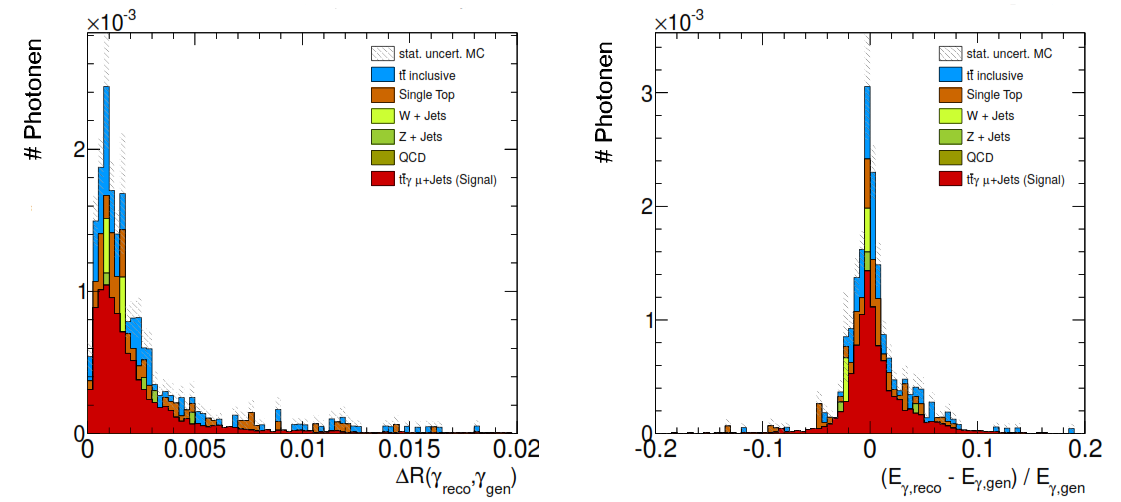
\includegraphics[width=\columnwidth]{bilder/matching}%
\caption{Links: $\Delta R$ des rekonstruierten und generierten Photons. Rechts: Relative Energiedifferenz der Photonen. Beide Verteilungen sind auf $\mathcal L_{int} = 1$\,pb$^{-1}$ normiert.}%
\label{fig:matching}%
\end{figure}

\begin{figure}%
\centering
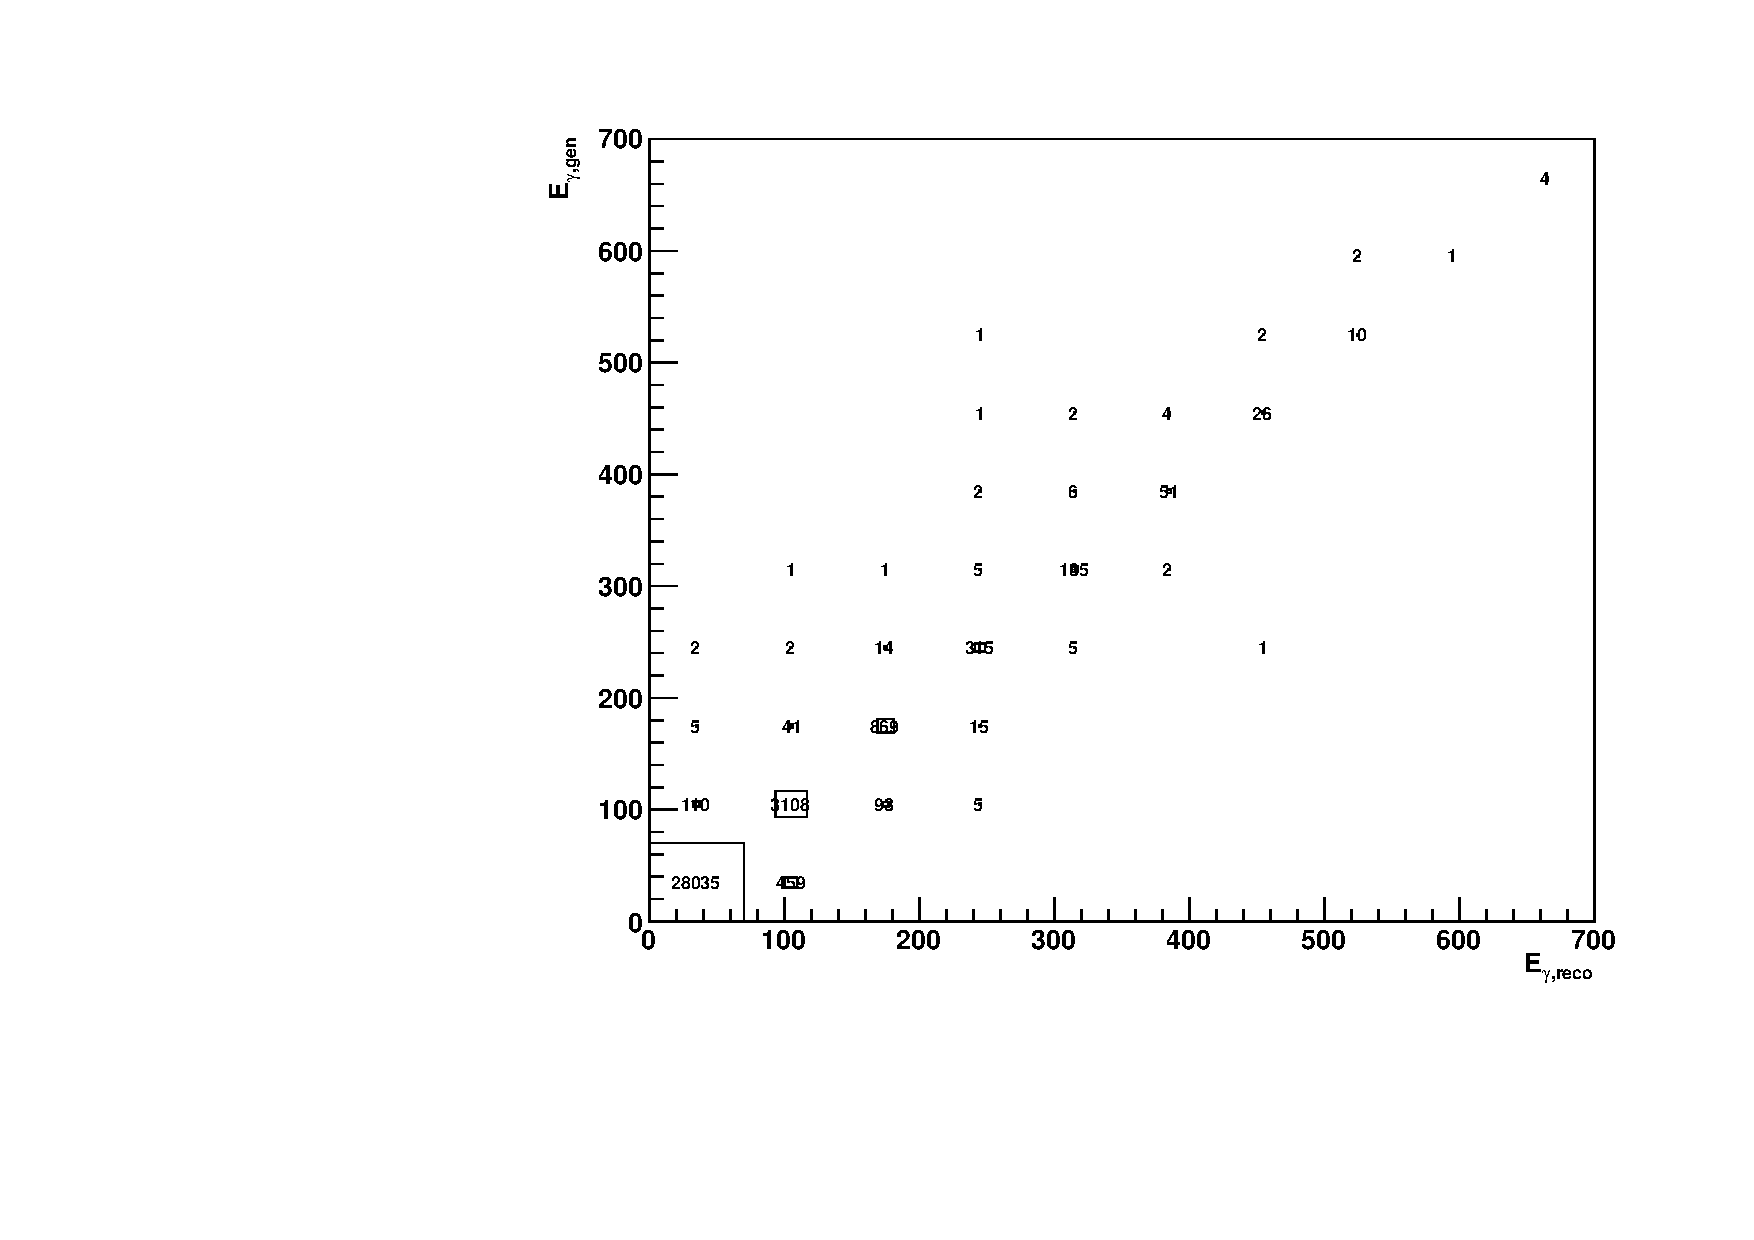
\includegraphics[width=0.5\columnwidth]{bilder/migration}%
\caption{Migrationsmatrix der Energie von generierten und rekonstruierten Photonen.}%
\label{fig:migration}%
\end{figure}

\subsection{Selektion von \texorpdfstring{$t\overline{t}+\gamma$}{ttg}-Ereignissen}
\label{sec:ttg_selektion}

Im folgenden werden die Erfordernisse an die Photonen im Endzustand beschrieben. Diese setzen sich aus Schnitten zusammen, die spezifisch f�r diese Analyse sind, sowie aus Forderungen, die auf einer CMS Empfehlung f�r Photon-Selektion basieren (\enquote{Photon-ID}, \cite{CMS:WZProduction}). \\
W�hrend der Photon-Selektion werden vor jedem Schnitt Kontrollplots erstellt, welche die Verteilung der jeweiligen Schnittvariable zeigen. In den Abbildungen \ref{fig:eta_et} bis \ref{fig:hollowconetrackiso_jurassicecaliso} sind einige dieser Verteilungen f�r das $d_A^{\gamma} = 0$-Szenario gezeigt. Im Anhang \ref{sec:kontrollplots} finden sich alle Kontrollplots in linearer und logarithmischer Auftragung f�r das $d_A^{\gamma} = 0$-Szenario.

\begin{figure}%
\centering
\begin{subfigure}[b]{0.48\textwidth}
  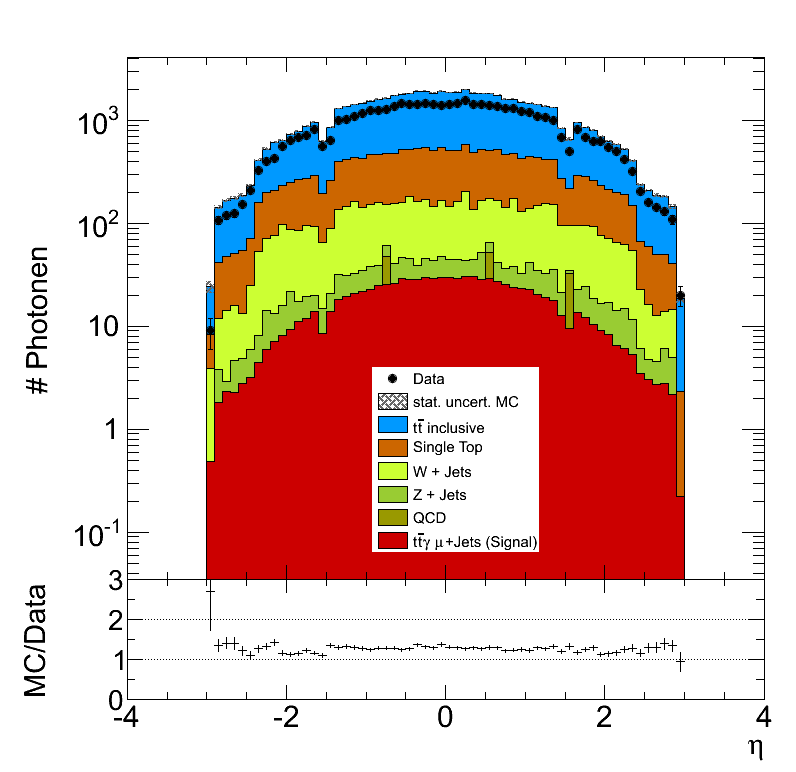
\includegraphics[width=\textwidth]{bilder/eta_log}%
\end{subfigure}
\begin{subfigure}[b]{0.48\textwidth}
  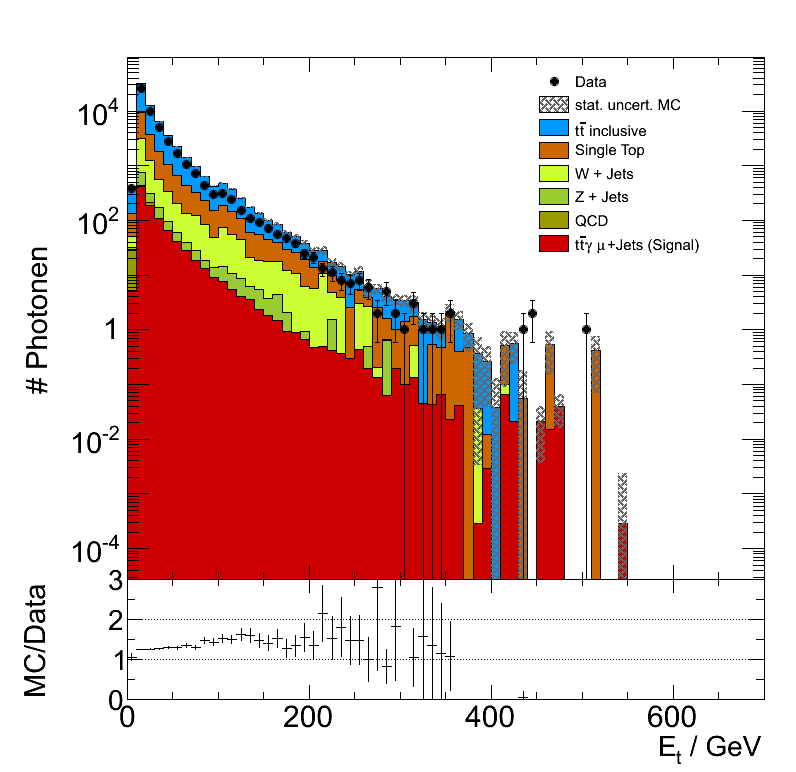
\includegraphics[width=\textwidth]{bilder/et_log}%
\end{subfigure}
\caption{Links: $\eta$-Verteilung des Photons. Forderung: $\left|\eta\right| < 1,4442$ und $1,556 < \left|\eta\right| < 2,4$. Rechts: $E_T$-Verteilung des Photons. Forderung: $E_T > 20$\,GeV}%
\label{fig:eta_et}%
\end{figure}

\subsubsection{Analyse-spezifische Schnitte}

\begin{description}
  \item[$\eta$-Bereich] Nur Photonen im Bereich von $\left|\eta\right|<1,4442$ und $1,556<\left|\eta\right|<2,5$ werden ber�cksichtigt, um sicherzustellen, dass der elektromagnetische Schauer des Photons im ECAL komplett rekonstruiert wurde.
  \item[Transversale Energie] Ein Schnitt von $E_T>20$\,GeV auf die transversale Energie des Photons wird angewandt, um falsch rekonstruierte Photonen und Photonen, die nicht aus dem Prim�rvertex stammen, zu unterdr�cken.
	\item[$\Delta R$(Photon, Myon)] Eine minimale Distanz von $\Delta R(\gamma,\mu)>0,3$ in der $\eta-\Phi$-Ebene wird gefordert, um Photonen, die vom hochenergetischen Myon abgestrahlt werden, auszuschlie�en.
	\item[$\Delta R$(Photon, Jet)] Der Jet-Algorithmus bezieht sehr oft Photonen in die rekonstruierten Jets ein. Deshalb werden alle Photonen im Bereich von $0,15<\Delta R(\gamma,\text{jet})<0,5$ nicht ber�cksichtigt, die obere Ausschlussgrenze repr�sentiert dabei den Jet-Radius von $\Delta R_{kt}=0,5$. Photon-Kandidaten innerhalb von $\Delta R < 0,15$ werden im n�chsten Schnitt gesondert behandelt.
	\item[Verh�ltnis von $E_{T,\gamma}$ zu $p_{T,Jet}$] Photonen im Bereich von $\Delta R < 0,15$ werden hinsichtlich des Verh�ltnisses von transversaler Energie des Photons zum transversalen Impuls des Jets weiter untersucht. Es wird angenommen, dass sich die Jets in diesem Bereich haupts�chlich aus dem Photon und niederenergetischer hadronischer Aktivit�t zusammensetzen, und dass die Photonen, bei denen der Einfluss der hadronischen Aktivit�t die pr�zise Messung des ECAL beeintr�chtigt, von den weiter unten besprochenen Photon-Identifikationsschnitten weitestm�glich herausgefiltert werden. Photon-Kandidaten mit einem Verh�ltnis von $E_{T,\gamma}/p_{T,Jet}>75\%$ werden akzeptiert.
\end{description}

\begin{figure}%
\centering
\begin{subfigure}[b]{0.48\textwidth}
  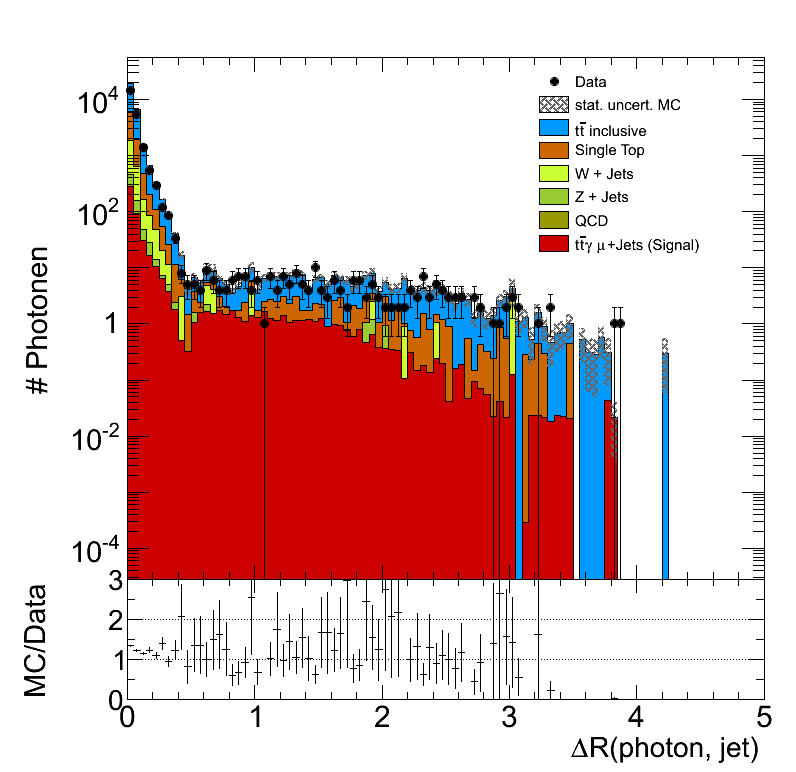
\includegraphics[width=\textwidth]{bilder/drjet_log}%
\end{subfigure}
\begin{subfigure}[b]{0.48\textwidth}
  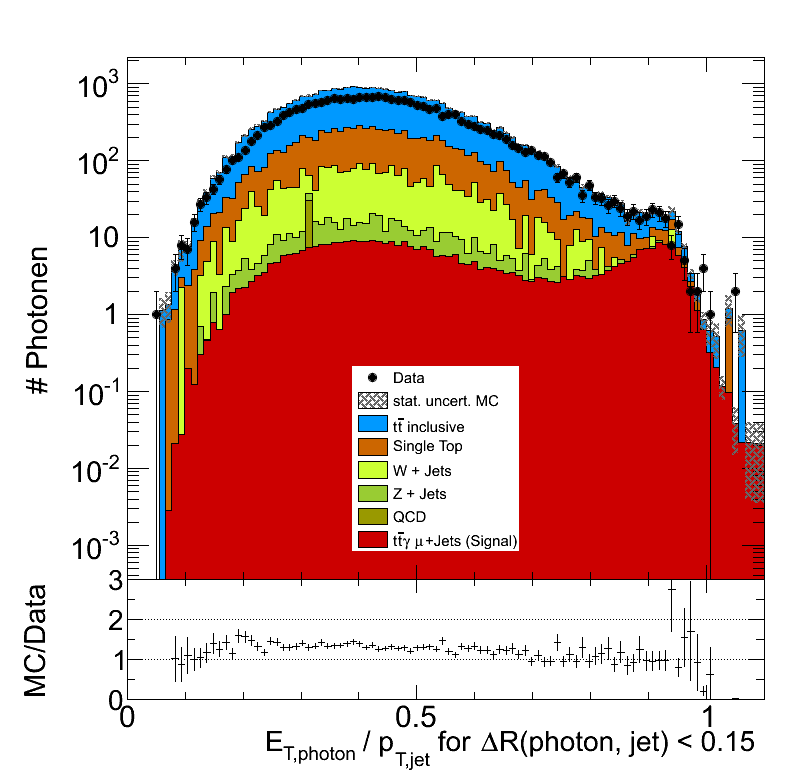
\includegraphics[width=\textwidth]{bilder/ptreldrjet_log}%
\end{subfigure}
\caption{Links: $\Delta R(\gamma,\text{jet})$-Verteilung des Photons. Forderung: $\Delta R(\gamma,\text{jet}) < 0,15$ oder $\Delta R(\gamma,\text{jet}) > 0,5$. Rechts: $E_{T,\gamma}/p_{T,jet}$-Verteilung des Photons f�r Photonen innerhalb von $\Delta R(\gamma,\text{jet}<0,15$. Forderung: $E_{T,\gamma}/p_{T,jet} > 0,75$.}%
\label{fig:drjet_ptreldrjet}%
\end{figure}

\subsubsection{Photon-Identifikationsschnitte}

\begin{description}
  \item[\enquote{pixel seed} Veto] Das Photon darf keinen \enquote{track seed} im Pixeldetektor haben.
	\item[Spurisolation] Die \enquote{Hollow Cone Track Isolation} $\Sigma_{trk}$ addiert den transversalen Impuls der Spuren im Siliziumspurdetektor in einem Kegel von $0,04<\Delta R<0,4$. Dieser Kegel ist hohl, um Photonen aus Paarerzeugung zu erlauben. Photonen in einem Bereich von $\Sigma_{trk}<2,0+0,001\cdot E_T/GeV$ werden akzeptiert.
	
\begin{figure}%
\centering
\begin{subfigure}[b]{0.48\textwidth}
  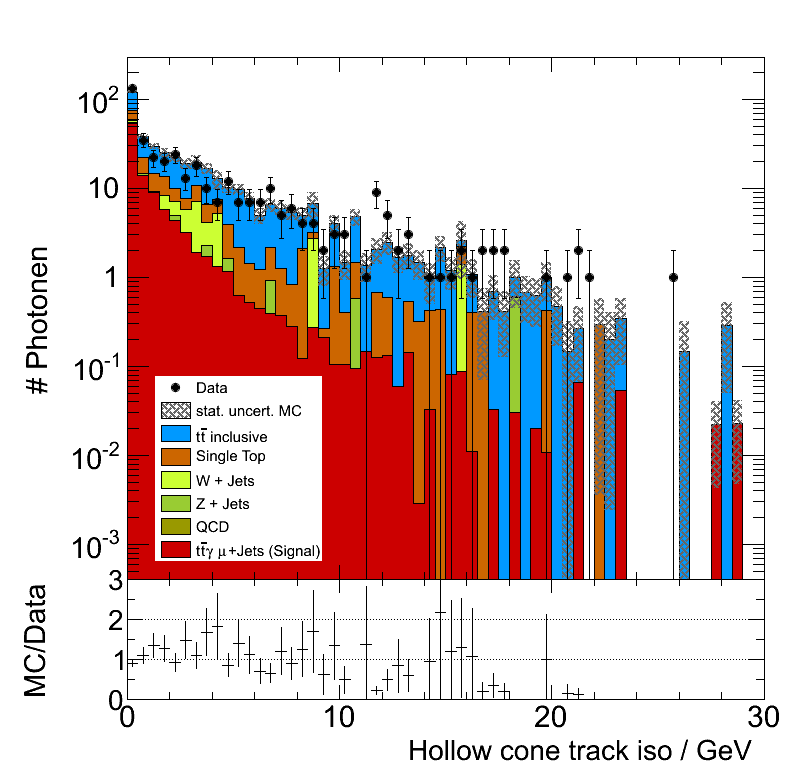
\includegraphics[width=\textwidth]{bilder/hollowconetrackiso_log}%
\end{subfigure}
\begin{subfigure}[b]{0.48\textwidth}
  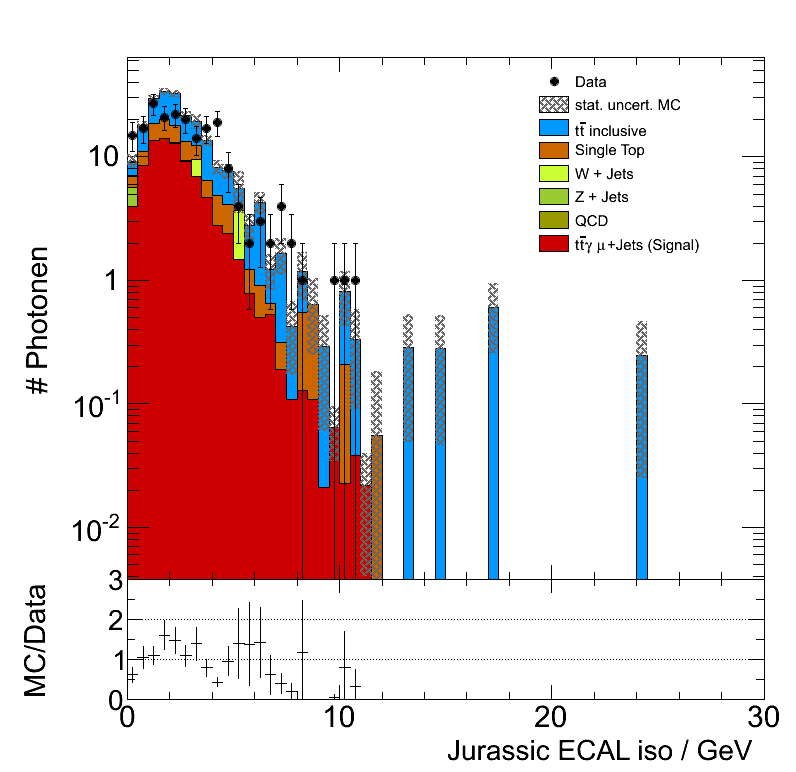
\includegraphics[width=\textwidth]{bilder/jurassicecaliso_log}%
\end{subfigure}
\caption{Links: Spur-Isolations-Verteilung des Photons. Forderung: $\Sigma_{trk} < 2,0 + 0,001\cdot E_T$. Rechts: ECAL-Isolations-Verteilung des Photons. Forderung: $\Sigma_{ECAL} < 4,2 + 0,006\cdot E_T$.}%
\label{fig:hollowconetrackiso_jurassicecaliso}%
\end{figure}
		
	\item[ECAL Isolation] Die \enquote{Jurassic ECAL Isolation} $\Sigma_{ECAL}$ ist ein Hohlkegel mit $0,06<\Delta R<0,4$. Zus�tzlich wird ein rechteckiger Bereich mit den Abmessungen $\Delta \eta \times \Delta \Phi =0,04\times 0,4$ um die Richtung des Photons nicht f�r die Berechnung der Isolation hinzugezogen, siehe Abb. \ref{fig:jurassic_ecal}. Dieser Schnitt fordert einen Wert von $\Sigma_{ECAL}<4,2+0,006\cdot E_T/GeV$
	
\begin{figure}%
\centering
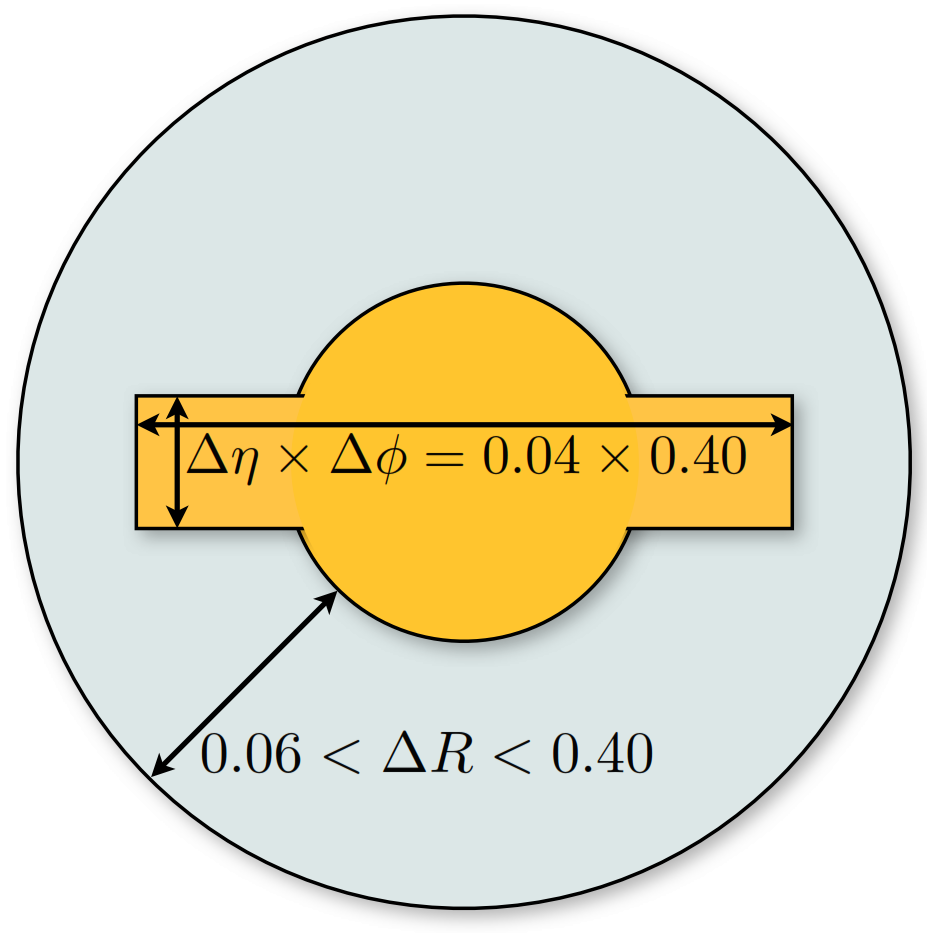
\includegraphics[width=0.3\columnwidth]{bilder/jurassic_ecal}%
\caption{Skizze zur \enquote{Jurassic ECAL Isolation}. Der zentrale Bereich wird f�r die Berechnung der Isolation nicht ber�cksichtigt. \cite{Tholen:Master}.}%
\label{fig:jurassic_ecal}%
\end{figure}	
	
	\item[HCAL Isolation] Die \enquote{Tower-based HCAL Isolation} $\Sigma_{HCAL}$ summiert �ber die deponierte Energie in allen HCAL towers innerhalb $\Delta R<0,4$ auf, dabei werden die towers hinter angesprochenen ECAL Clustern nicht ber�cksichtigt, mit diesen befasst sich der n�chste Schritt. Die Photonen m�ssen die Forderung $\Sigma_{HCAL}<2,2+0,0025\cdot E_T/GeV$ erf�llen.
	\item[Verh�ltnis HCAL/ECAL] Die Energiedeposition in HCAL towers hinter den zugeh�rigen ECAL Clustern darf maximal 5\% sein.
	\item[Weite des Superclusters] $\sigma_{i\eta i\eta}$ bezeichnet die Energie-gewichtete Aufspreizung des ECAL Superclusters in Richtung von $\eta$. Diese ist wie folgt definiert:
	
\begin{equation}
\sigma_{i\eta i\eta}=\left(\frac{\sum(\eta_i-\overline{\eta})^2\omega_i}{\sum \omega_i}\right)^{1/2} \ ; \ \overline{\eta}=\frac{\sum \eta_i\omega_i}{\sum \omega_i} \ ; \ \omega_i=\text{max}\left(0;4,7+log\frac{E_i}{E_{5\times 5}}\right) \ .
\end{equation}	

Hier ist $E_i$ die in einem einzelnen ECAL-Kristall deponierte Energie und $E_{5\times 5}$ die Summe der Energiedepositionen in einem Cluster von 5 $\times$ 5 Kristallen um den h�chste Energieeintrag herum. Photonen aus dem harten Prozess haben eine kleinere Schauerweite im ECAL als missidentifizierte Photonen. Die Forderung an die Schauerweite ist $\sigma_{i\eta i\eta}<0,011$ im Bereich von $\left|\eta\right|<1,5$ und $\sigma_{i\eta i\eta}<0,03$ f�r $\left|\eta\right|>1,5$.

\end{description}

Im allgemeinen zeigen die Schnittvariablen eine gute �bereinstimmung in der Form der Verteilung zwischen Daten- und Monte-Carlo-Ereignissen. Das Signal-zu-Untergrund-Verh�ltnis der $t\overline{t} + \gamma$-Selektion liegt bei $S/B = 0,53$, die Selektionseffizienz betr�gt $\epsilon_{\gamma} = 23\%$. 134 Ereignisse aus experimentellen Daten werden selektiert. \\
Abbildung \ref{fig:cutflow} zeigt den sogenannten \enquote{cutflow} der Photon-Selektion f�r das $d_A^{\gamma} = 0$-Szenario. Er beschreibt den Verlauf der Selektion f�r Monte-Carlo- und Datenereignisse. Die Ereignisse aus Monte-Carlo-Simulationen sind hier auf die integrierte Luminosit�t der experimentellen Daten normiert. Man erkennt, dass vor der Photon-Selektion durch Monte-Carlo-Simulationen mehr Ereignisse vorhergesagt werden als in experimentellen Daten aufgezeichnet wurden. Nach der Selektion sind jedoch mehr Datenereignisse vorhanden wie vorhergesagt. Der �bergang vom Monte-Carlo �berschuss zu einem Monte-Carlo Defizit findet im Selektionsschritt \enquote{Verh�ltnis von $E_{T,\gamma}$ zu $p_{T,Jet}$} statt. Dies weist auf eine Diskrepanz zwischen Monte-Carlo-Simulation und experimentellen Daten hin, die in weiteren Studien n�her untersucht werden sollte. Eine m�gliche Ursache f�r diese Diskrepanz k�nnte beispielsweise die Jet-Simulation oder das angewandte Hadronisierungsmodell sein. Der Fokus dieser Analyse liegt jedoch weniger auf der Messung der totalen Rate, also des Wirkungsquerschnittes, sondern auf der Analyse der $E_T$-Verteilung. Diese ist jedoch weitestgehend unabh�ngig von der Normierung, siehe Abbildung \ref{fig:eta_et} rechts.\\
Die gesamte Selektionseffizienz betr�gt f�r Monte-Carlo-Ereignisse $\epsilon_{\gamma}^{ges, MC} \approx 0,42\%$ und f�r experimentell aufgezeichnete Daten $\epsilon_{\gamma}^{ges, Data} \approx 0,61\%$. 


\begin{figure}%
\centering
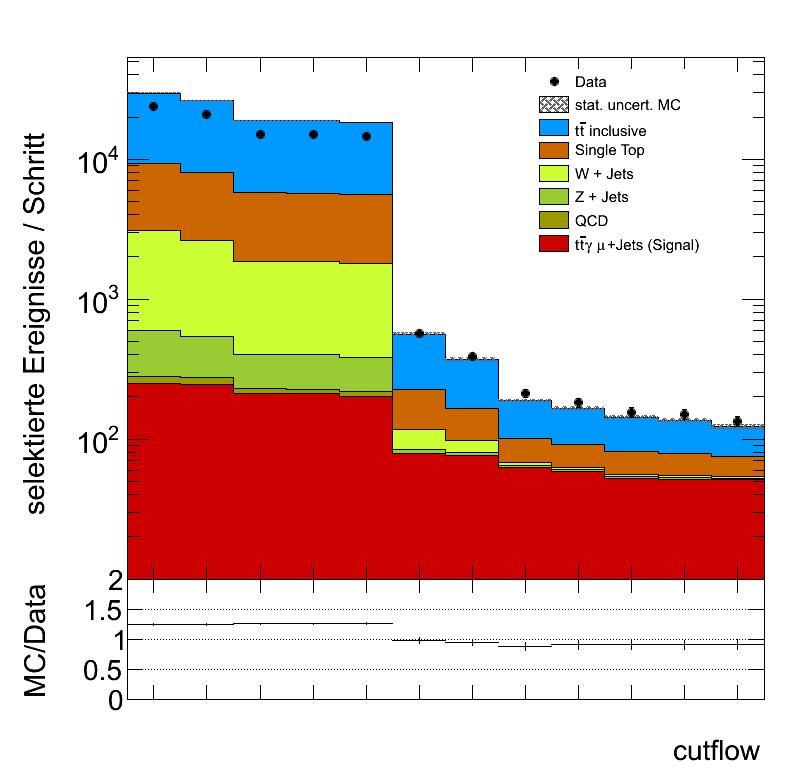
\includegraphics[width=0.5\columnwidth]{bilder/cutflow}%
\caption{Cutflow der Photon-Selektion in halblogarithmischer Auftragung. Jedes Bin zeigt hier die Anzahl der selektierten Ereignisse im jeweiligen Selektionsschritt.}%
\label{fig:cutflow}%
\end{figure}

%
%
% Kapitel MC-Studien
%
%


\chapter{Studie der von WHIZARD generierten Monte-Carlo-Samples}

Die Studie der von WHIZARD generierten Monte-Carlo-Daten soll zeigen, wie sich der Wirkungsquerschnitt des $t\overline{t}+\gamma$-Prozesses sowie das $E_T$-Spektrum der Photonen aus dem harten Prozess durch Variation des angenommenen $d_A^{\gamma}$-Wertes ver�ndert. Des weiteren soll untersucht werden, welche Variable sich am besten dazu eignet, zwischen verschiedenen $d_A^{\gamma}$-Szenarien zu unterscheiden. Durch Verwendung von Generatorteilchen werden Aufl�sungseffekte durch die Rekonstruktion sowie Akzeptanzeffekte durch die Selektion vernachl�ssigt.

\section{Wirkungsquerschnitt des \texorpdfstring{$t\overline{t}+\gamma$}{ttg}-Prozesses}
\label{sec:wq}

Es wird eine quadratische Abh�ngigkeit des Wirkungsquerschnittes vom Parameter $d_A^{\gamma}$ erwartet, da $d_A^{\gamma}$ linear in das Matrixelement eingeht und der Wirkungsquerschnitt proportional zum Quadrat des Matrixelementes ist. \\
Mit dem Leading-Order-Monte-Carlo-Generator WHIZARD in der Version 2.1.1 werden f�r Werte f�r das elektrische Dipolmoment von $0<d_A^{\gamma}<1$ in Schritten von 0,01 zun�chst die Matrixelemente f�r den harten Prozess generiert. Der Ansatz $2 \rightarrow 5$ wird implementiert mit zwei W-Bosonen, zwei b-Quarks und einem Photon im Endzustand. Die Matrixelement-Berechnung wird abgebrochen, wenn ein Fehler auf den Wirkungsquerschnitt von unter 1\% errechnet wird. Die so berechneten Wirkungsquerschnitte sind in Abb. \ref{fig:cs_wofit} links dargestellt. Man erkennt die erwartete quadratische Abh�ngigkeit. Fittet man eine quadratische Funktion an die Verteilung (Abb. \ref{fig:cs_wofit}), wird diese Abh�ngigkeit noch deutlicher. Auff�llig ist der gro�e Fehler auf den Wirkungsquerschnitt bei den Werten $d_A^{\gamma}=0,06$ und $d_A^{\gamma}=0,95$. Dieser l�sst sich auch bei deutlich l�ngerer Berechnung des Matrixelements nicht weiter verringern.

\begin{figure}%
\centering
\begin{subfigure}[b]{0.4\textwidth}
  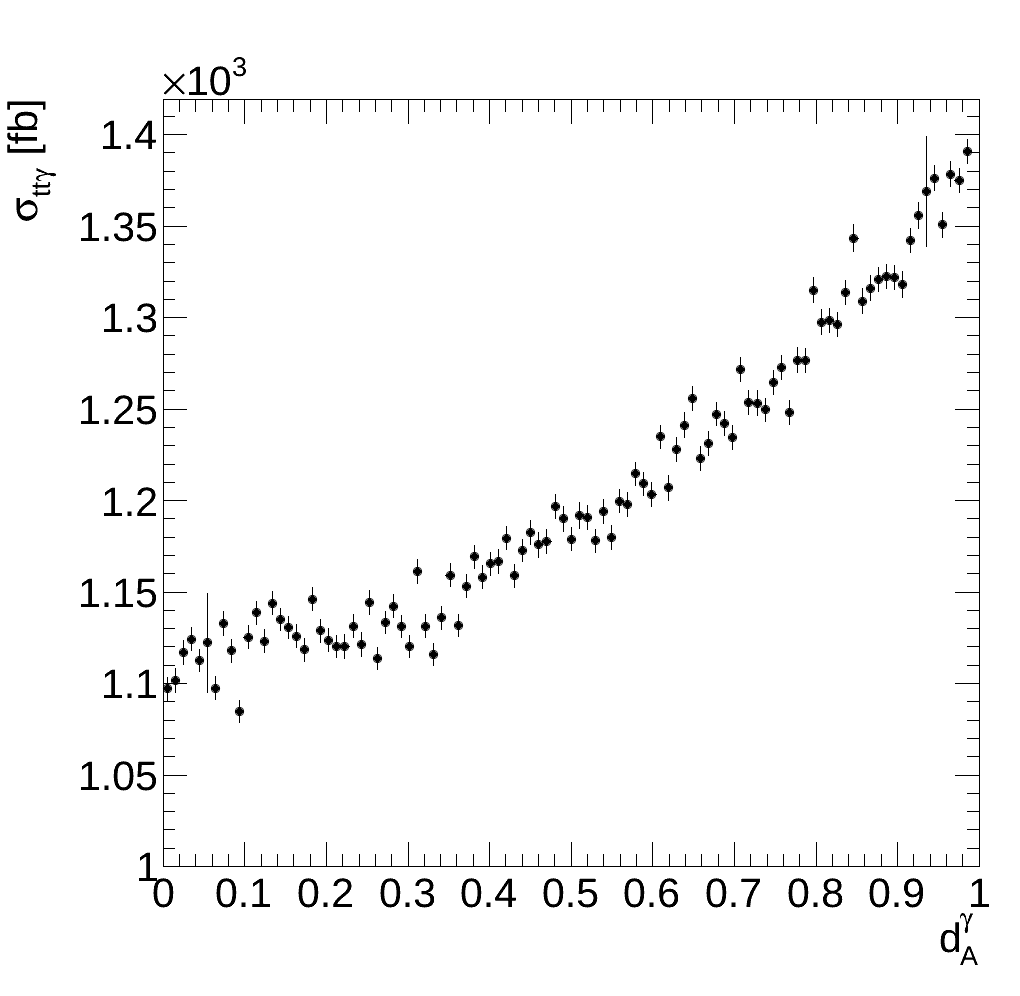
\includegraphics[width=\textwidth]{bilder/csplotwofit}%
\end{subfigure}
\hspace{0.1\textwidth}
\begin{subfigure}[b]{0.4\textwidth}
  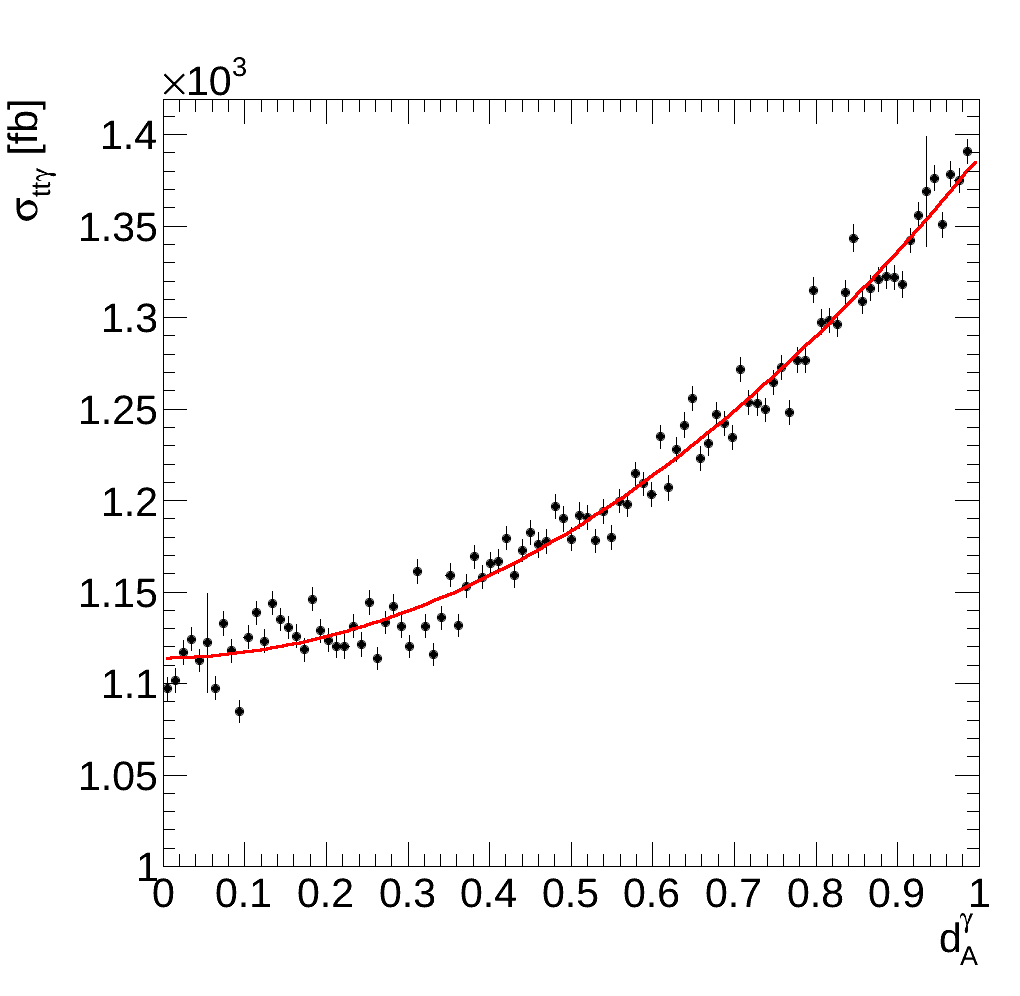
\includegraphics[width=\textwidth]{bilder/crosssectionplot}%
\end{subfigure}	
\caption{Wirkungsquerschnitt des $t\overline{t}+\gamma$-Prozesses f�r $0<d_A^{\gamma}<1$, rechts mit eingezeichneter Fit-Funktion}%
\label{fig:cs_wofit}%
\end{figure}

\section{\texorpdfstring{$E_T$}{ET}-Spektrum des Photons}

Aus dem berechneten Matrixelement werden nun f�r jeden $d_A^{\gamma}$-Wert 105.000 Ereignisse generiert und im Les-Houches-Event Format (LHEF) abgespeichert \cite{Alwall:LesHouches}. Es wird f�r ein h�heres elektrisches Dipolmoment ein h�rteres Photonspektrum erwartet. Um dies zu verifizieren, gibt es mehrere Ans�tze, die im Folgenden erl�utert werden sollen.

\subsection{2-Bin-Analyse}

Das $E_T$-Spektrum wird in zwei Bereiche aufgeteilt. Der erste Bereich reicht von 50\,GeV bis 100\,GeV, der zweite von 100\,GeV bis 200\,GeV, siehe dazu Abb. \ref{fig:2bin_skizze}. Nun wird das Verh�ltnis der Anzahl der Photonen in den beiden Bereichen gegen $d_A^{\gamma}$ aufgetragen, siehe Abb. \ref{fig:2bin_plot}. Auf der linken Seite sieht man zwei Messwerte, die nicht dem allgemeinen Verlauf folgen. Dies sind die schon in Kapitel \ref{sec:wq} angesprochenen Messpunkte, die durch irreduzibel gro�e Fehler auf den Wirkungsquerschnitt auffielen und auch in allen anderen Analysemethoden herausstechen. Es scheint sich hier um einen Fehler in der Matrixelementberechnung von WHIZARD zu handeln, die Punkte $d_A^{\gamma}=0,06$ und $d_A^{\gamma}=0,95$ werden im folgenden f�r die Auswertung der verschiedenen Analysemethoden nicht ber�cksichtigt. In Abb. \ref{fig:2bin_plot} rechts ist eine polynomische Funktion zweiten Grades an die Verteilung gefittet. Man erkennt eine gute �bereinstimmung des Fits mit den Messwerten, die sich am Wert von $\chi^2/ndf=105,3/96$ ablesen l�sst.

\begin{figure}%
\centering
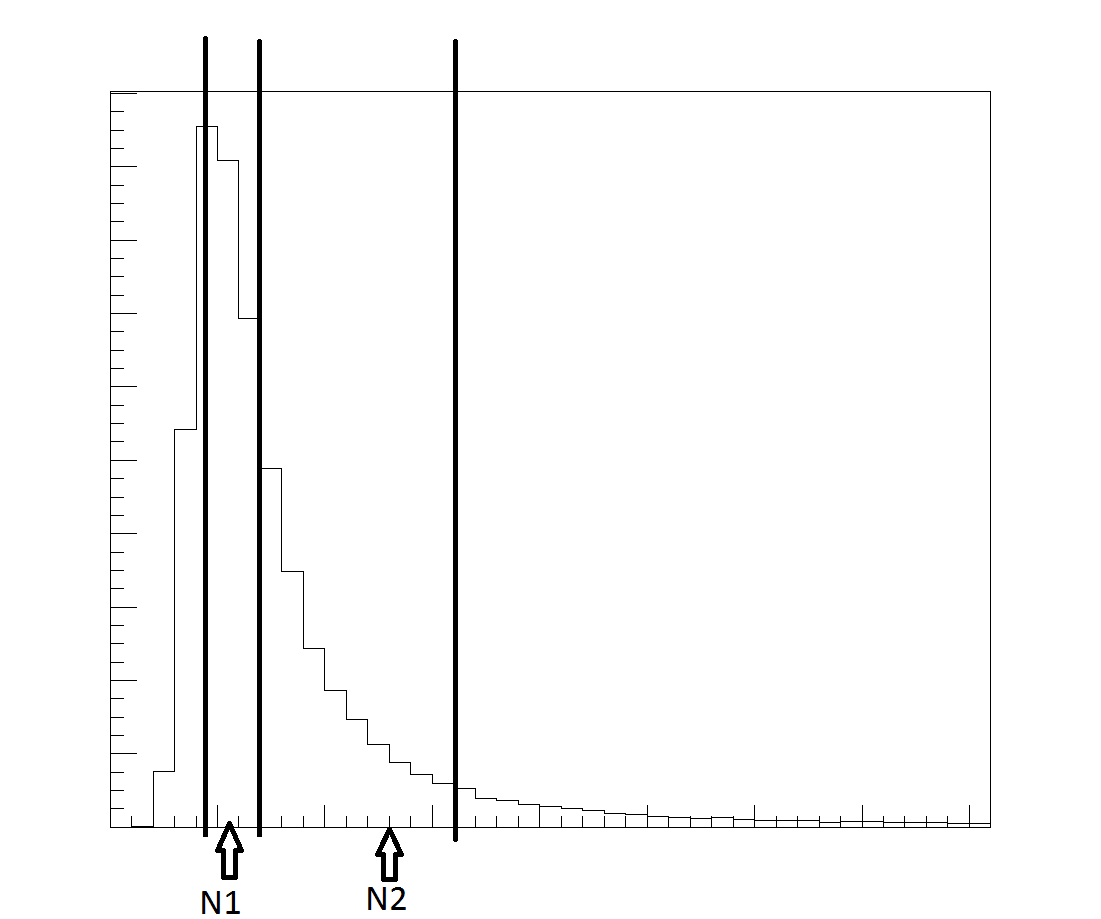
\includegraphics[width=0.5\columnwidth]{bilder/2binskizze}%
\caption{Schema der Unterteilung bei der 2-Bin-Analyse.}%
\label{fig:2bin_skizze}%
\end{figure}

\begin{figure}%
\centering
\begin{subfigure}[b]{0.4\textwidth}
  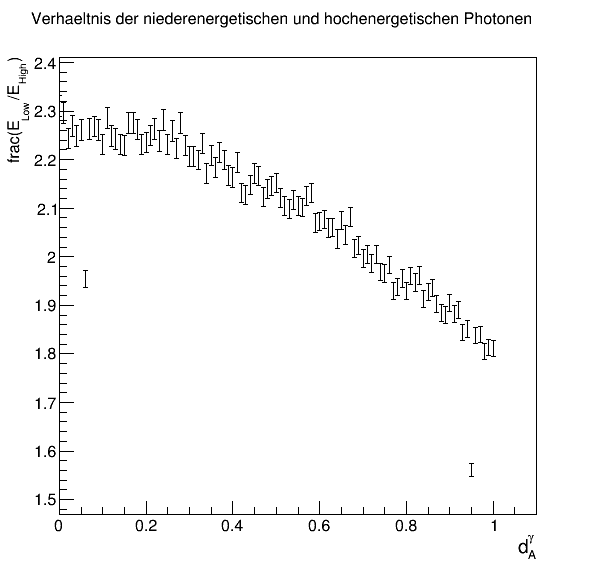
\includegraphics[width=\textwidth]{bilder/twobinplot}%
\end{subfigure}
\hspace{0.1\textwidth}
\begin{subfigure}[b]{0.4\textwidth}
  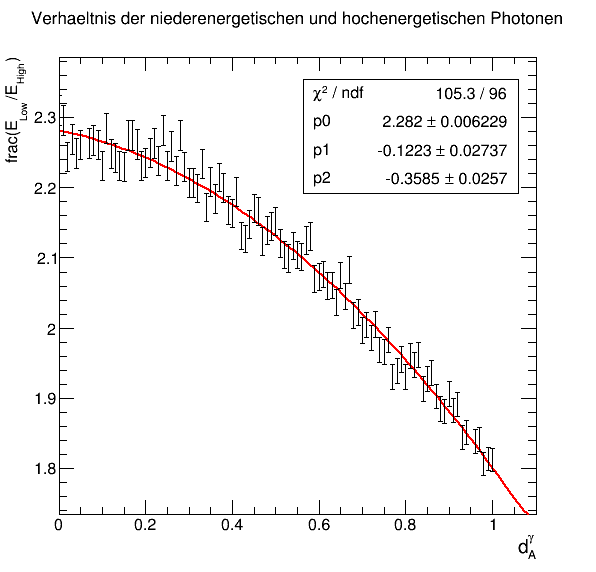
\includegraphics[width=\textwidth]{bilder/twobinfit}%
\end{subfigure}
\caption{Verh�ltnis der Anzahl der Photonen in Bin 1 und Bin 2.}%
\label{fig:2bin_plot}%
\end{figure}

\subsection{\texorpdfstring{$E_T$}{ET}-Mean-Analyse}

In diesem Ansatz wird der Schwerpunkt der $E_T$-Verteilung betrachtet, siehe Abb. \ref{fig:mean_skizze}, dies ist der gewichtete Mittelwert dieser Verteilung. Mithilfe der Analysesoftware ROOT \cite{Brun:Root} wird dieser Parameter und dessen Fehler ermittelt und gegen $d_A^{\gamma}$ aufgetragen. Diese Auftragung ist in Abb. \ref{fig:mean_plot} zu sehen. Wieder sieht man in der linken Verteilung die oben angesprochenen Punkte, die f�r den Fit im rechten Bild unber�cksichtigt blieben. Auch hier wurde eine Polynom zweiten Grades angefittet. die �bereinstimmung dieses Fits ist in dieser Analysemethode etwas schlechter, was damit zusammenh�ngen kann, dass die Fehler auf den Schwerpunkt der $E_T$-Verteilung von ROOT als zu klein angenommen werden. 

\begin{figure}%
\centering
\includegraphics[width=0.5\columnwidth]{bilder/meanskizze}%
\caption{Schema der $E_T$-Mean-Analyse.}%
\label{fig:mean_skizze}%
\end{figure}

\begin{figure}%
\centering
\begin{subfigure}[b]{0.4\textwidth}
  \includegraphics[width=\textwidth]{bilder/meanplot}%
\end{subfigure}
\hspace{0.1\textwidth}
\begin{subfigure}[b]{0.4\textwidth}
  \includegraphics[width=\textwidth]{bilder/meanfit}%
\end{subfigure}
\caption{Verlauf des Schwerpunktes der $E_T$-Verteilung.}%
\label{fig:mean_plot}%
\end{figure}

\subsection{Analyse der Einh�llenden der \texorpdfstring{$E_T$}{ET}-Verteilung}

\begin{figure}%
\centering
\includegraphics[width=0.5\columnwidth]{bilder/slopeskizze}%
\caption{Skizze zum Prinzip der Analyse der Einh�llenden.}%
\label{fig:slope_skizze}%
\end{figure}

Hier wird schlie�lich die Einh�llende der $E_T$-Verteilung betrachtet. Wie in Abb. \ref{fig:slope_skizze} zu sehen ist, kann die Verteilung im Bereich zwischen 100\,GeV und 225\,GeV durch eine logarithmische Funktion

\begin{equation}
N(x) = N_0\cdot e^{\lambda \cdot x}
\end{equation}

beschrieben werden. F�r jeden $d_A^{\gamma}$-Wert wird nun an das $E_T$-Spektrum eine Exponentialfunktion angefittet und der Wert von $\lambda$ gegen $d_A^{\gamma}$ aufgetragen. Dieser Plot ist in Abb. \ref{fig:slope_plot} zu sehen. Man erkennt im linken Bild eine Korrelation zwischen dem Parameter $\lambda$ der Exponentialfunktion und dem elektrischen Dipolmoment $d_A^{\gamma}$. Es wird eine $x^3$-Abh�ngigkeit angenommen und der rechte Plot in \ref{fig:slope_plot} zeigt einen Fit mit einem Polynom dritten Grades. Auch hier ist die �bereinstimmung des Fits mit den Datenpunkten sehr gut, es ergibt sich ein $\chi^2/ndf$ von $94,56/95$.

\begin{figure}%
\centering
\begin{subfigure}[b]{0.4\textwidth}
  \includegraphics[width=\textwidth]{bilder/slopeplot}%
\end{subfigure}
\hspace{0.1\textwidth}
\begin{subfigure}[b]{0.4\textwidth}
  \includegraphics[width=\textwidth]{bilder/slopefit}%
\end{subfigure}
\caption{Verlauf der Einh�llenden der $E_T$-Verteilung.}%
\label{fig:slope_plot}%
\end{figure}


%
%
% Kapitel Datenstudie
%
%


\chapter{Vergleich der Monte-Carlo-Simulationen mit Daten}

\section{\texorpdfstring{$E_T$}{ET}-Spektren}

F�r elf der in Kapitel \ref{sec:montecarlo} erzeugten WHIZARD-Sample ($0\leq d_A^{\gamma} \leq 1$, Schritte von 0,1) werden nun die Hadronisierung und die Detektorantwort simuliert, die Rekonstruktionsalgorithmen darauf angewendet (siehe Abschnitt \ref{sec:reco}) sowie die in den Abschnitten \ref{sec:vorselektion} respektive \ref{sec:ttg_selektion} beschriebenen Selektionen durchgef�hrt. Die jeweiligen $E_T$-Spektren werden aufgetragen. Abb. \ref{fig:et_galerie} zeigt einige dieser Spektren in logarithmischer Auftragung, die $y$-Achse ist hier auf die Luminosit�t normiert. Man erkennt, dass wie erwartet das Spektrum mit steigendem $d_A^{\gamma}$ h�rter wird, sich also zu h�herenergetischen Photonen verschiebt. Dies l�sst sich auch in Abb. \ref{fig:et_kombi} erkennen, in der dre dieser Energiespektren �bereinandergeplottet sind. Des weiteren erkennt man eine Zunahme der Anzahl der rekonstruierten und selektierten Photonen mit steigender Kopplungsst�rke. Dies kommt zum einen daher, dass die $t\overline{t}+\gamma$-Selektion niederenergetische Photonen unterdr�ckt, zum anderen kann man hier auch auf eine Abh�ngigkeit des Wirkungsquerschnittes des Prozesses von $d_A^{\gamma}$ schliessen, siehe \ref{sec:wq}. \\

\begin{figure}%
\begin{subfigure}[b]{0.4\textwidth}
\includegraphics[width=\textwidth]{bilder/et_0}%
\end{subfigure}
\hspace{0.1\textwidth}
\begin{subfigure}[b]{0.4\textwidth}
\includegraphics[width=\textwidth]{bilder/et_02}%
\end{subfigure}

\begin{subfigure}[b]{0.4\textwidth}
\includegraphics[width=\textwidth]{bilder/et_04}%
\end{subfigure}
\hspace{0.1\textwidth}
\begin{subfigure}[b]{0.4\textwidth}
\includegraphics[width=\textwidth]{bilder/et_06}%
\end{subfigure}

\begin{subfigure}[b]{0.4\textwidth}
\includegraphics[width=\textwidth]{bilder/et_08}%
\end{subfigure}
\hspace{0.1\textwidth}
\begin{subfigure}[b]{0.4\textwidth}
\includegraphics[width=\textwidth]{bilder/et_1}%
\end{subfigure}
\caption{$E_T$-Verteilungen von rekonstruierten und selektierten Monte-Carlo-Daten f�r verschiedene Werte von $d_A^{\gamma}$.}%
\label{fig:et_galerie}%
\end{figure}

\begin{figure}%
\centering
\includegraphics[width=0.4\columnwidth]{bilder/platzhalter}%
\caption{$E_T$-Spektren bei $d_A^{\gamma}=$0; 0,5 und 1.}%
\label{fig:et_kombi}%
\end{figure}

\section{Exponentieller Fit an die \texorpdfstring{$E_T$}{ET}-Spektren}

Von den in Kapitel \ref{sec:montecarlo} vorgestellten Analysemethoden, um den Wert von $d_A^{\gamma}$ anhand von Daten einzugrenzen, wird hier exemplarisch die Analyse der Einh�llenden der $E_T$-Verteilung der Photonen besprochen. Dazu wird nun an die prozessierten Monte-Carlo-Simulationen eine Exponentialfunktion

\begin{equation}
N(x) = N_0\cdot e^{\lambda \cdot x}
\end{equation}

 angefittet, siehe Abb. \ref{fig:fit_galerie}. Der Fitbereich liegt zwischen dem Bin mit der maximalen Anzahl der Eintr�ge bis 250\,GeV. Der Parameter$\lambda$ wird gegen $d_A^{\gamma}$ aufgetragen, siehe \ref{fig:et_slope}. Wie schon in Kapitel \ref{sec:ana_slope} wird nun ein Polynom dritten Grades an diese Datenpunkte gefittet, siehe Abb. \ref{fig:et_slopefit}. Man sieht, dass die Parameter ersten bis dritten Grades innerhalb der Unsicherheit des Fits mit Null vereinbar sind. Um dieser Problematik entgegenzuwirken, wird ein zweiter Ansatz mit einem linearen Fit gew�hlt. Dieser zeigt auch eine gute �bereinstimmung mit den Messwerten (Abb. \ref{fig:et_slopefit_linear}).  \\
In Abbildung \ref{fig:fehlerbandplot} sieht man die aus dem linearen Fit ermittelte Funktion $\lambda\left(d_A^{\gamma}\right) = p_1\cdot d_A^{\gamma} +p_0$ (mittlere Gerade). Die obere und untere Gerade beschreibt respektive die Funktion f�r $\lambda\left(d_A^{\gamma}\right) = (p_1+\Delta p_1)\cdot d_A^{\gamma} +(p_0+\Delta p_0)$ bzw. $\lambda\left(d_A^{\gamma}\right) = (p_1-\Delta p_1)\cdot d_A^{\gamma} +(p_0-\Delta p_0)$, das so gebildete Fehlerband umschliesst somit eine Standardabweichung.

\begin{figure}%
\begin{subfigure}[b]{0.4\textwidth}
\includegraphics[width=\textwidth]{bilder/fit_0}%
\end{subfigure}
\hspace{0.1\textwidth}
\begin{subfigure}[b]{0.4\textwidth}
\includegraphics[width=\textwidth]{bilder/fit_02}%
\end{subfigure}

\begin{subfigure}[b]{0.4\textwidth}
\includegraphics[width=\textwidth]{bilder/fit_04}%
\end{subfigure}
\hspace{0.1\textwidth}
\begin{subfigure}[b]{0.4\textwidth}
\includegraphics[width=\textwidth]{bilder/fit_06}%
\end{subfigure}

\begin{subfigure}[b]{0.4\textwidth}
\includegraphics[width=\textwidth]{bilder/fit_08}%
\end{subfigure}
\hspace{0.1\textwidth}
\begin{subfigure}[b]{0.4\textwidth}
\includegraphics[width=\textwidth]{bilder/fit_1}%
\end{subfigure}
\caption{Exponentieller Fit an die $E_T$-Verteilungen von rekonstruierten und selektierten Monte-Carlo-Daten f�r verschiedene Werte von $d_A^{\gamma}$.}%
\label{fig:fit_galerie}%
\end{figure}

\begin{figure}%
\centering
\includegraphics[width=0.4\columnwidth]{bilder/et_slope}%
\caption{Verlauf des $\lambda$-Parameters des Fits an die $E_T$-Spektren.}%
\label{fig:et_slope}%
\end{figure}

\begin{figure}%
\centering
\includegraphics[width=0.4\columnwidth]{bilder/et_slopefit}%
\caption{Fit eines Polynoms dritten Grades an den Verlauf des $\lambda$-Parameters.}%
\label{fig:et_slopefit}%
\end{figure}

\begin{figure}%
\centering
\includegraphics[width=0.4\columnwidth]{bilder/et_slopefit_linear}%
\caption{Linearer Fit an den Verlauf des $\lambda$-Parameters.}%
\label{fig:et_slopefit_linear}%
\end{figure}

\begin{figure}%
\centering
\includegraphics[width=0.4\columnwidth]{bilder/fehlerbandplot}%
\caption{Gefitteter Verlauf des $\lambda$-Wertes mit Fehlerband.}%
\label{fig:fehlerbandplot}%
\end{figure}

\section{Vergleich mit Daten}



%
%
% Kapitel Zusammenfassung
%
%


\chapter{Zusammenfassung und Ausblick}

Die Produktion von Top-Paaren in Verbindung mit einem Photon er�ffnet die M�glichkeit, die elektromagnetische Kopplung von isolierten Quarks zu untersuchen. Das Top-Quark stellt dabei ein einzigartiges Testobjekt dar, da es zerf�llt, bevor es hadronisieren kann. Damit wird die Suche nach Physik jenseits des Standardmodells erm�glicht. \\
Die hier vorgestellte Analyse untersucht die Separationsf�higkeit mehrerer Kenngr�ssen des Photon-$E_T$-Spektrums hinsichtlich verschiedener Kopplungsst�rken $d_A^{\gamma}$ des elektrischen Dipolmomentes. Die Untersuchung wird im semimyonischen Zerfallskanal von Top-Paaren mit einem zus�tzlichen Photon im Endzustand am CMS-Experiment durchgef�hrt. \\

F�r verschiedene $d_A^{\gamma}$-Szenarien werden mit dem NLO-Ereignisgenerator WHIZARD Matrixelemente berechnet und jeweils 105.000 $t\overline{t}+\gamma$-Ereignisse generiert. Die $E_T$-Spektren der harten Photonen dieser Ereignisse werden mittels dreier Analyseverfahren untersucht: einer 2-Bin-Analyse, der Analyse des gewichteten Mittelwertes der Verteilung und der Analyse einer Exponentialanpassung an das Spektrum. Die Variablen $E_{Low}/E_{High}$, $\overline{E_T}$ und $\lambda$ weisen auf Generatorniveau eine sehr gute Separationskraft auf. \\
Eine CMS Referenzselektion wird als $t\overline{t}$-Vorselektion implementiert, um Ereignisse im semimyonischen Top-Paar-Zerfallskanal zu erhalten. Darin wird ein hochenergetisches, isoliertes Myon und vier Jets gefordert, von denen einer b-artig ist. Ein Signal-zu-Untergrund-Verh�ltnis von $S/B = 2,24$ wird erreicht bei einer Selektionseffizienz von $\epsilon_{t\overline{t}} = 2,8\%$. \\
Zus�tzlich wird eine Photon-Selektion implementiert, Anforderungen an die Photonidentifikation werden hierbei von einer CMS Referenz �bernommen. Eine Selektionseffizienz f�r $t\overline{t}+\gamma$-Ereignisse von $\epsilon_{\gamma} = 23\%$ und ein Signal-zu-Untergrund-Verh�ltnis von $S/B = 0,53$ werden erreicht. Aus einem Datensatz von 2011 aufgezeichneten Daten, die einer integrierten Luminosit�t von 4,7\,fb$^{-1}$ entsprechen, werden $N_{sel} = 134$ $t\overline{t}+\gamma$-Ereignisse selektiert. F�r alle Schnittvariablen besteht in der Form der Verteilung eine gute �bereinstimmung zwischen experimentell gemessenen Daten und Daten aus Monte-Carlo-Simulationen.\\
Die $E_T$-Spektren der selektierten und rekonstruierten Photon-Kandidaten werden f�r verschiedene $d_A^{\gamma}$-Szenarien mit den gleichen Analyseverfahren wie auf Generatorniveau untersucht. Auch auf Rekonstruktionsniveau haben die untersuchten Variablen eine gute Separationskraft. Das $E_T$-Spektrum der 134 Photonen aus Datenereignissen wird analysiert und die Werte f�r $(E_{Low}/E_{High})_{Data}$, $\overline{E_T}_{Data}$ und $\lambda_{Data}$ mit den jeweiligen ermittelten Werten f�r die Monte-Carlo-$d_A^{\gamma}$-Szenarien verglichen. In allen untersuchten Kenngr��en sind die aus Daten ermittelten Werte mit dem Standardmodellwert von $d_A^{\gamma} = 0$ vereinbar. Es ergeben sich die Werte

\begin{alignat*}{2}
(E_{Low}/E_{High})_{Data} &= 5,09 & &\pm 1,19 \\
\overline{E_T}_{Data} &= 55,36 & &\pm 3,19\,GeV \\
\lambda_{Data} &= -0,0333 & &\pm 0,0037 \ .
\end{alignat*}


Systematische Unsicherheiten durch Generatoreffekte und Normalisierung der Signal- beziehungsweise Untergrund-Sample werden untersucht. Es ergeben sich f�r das Standardmodell-Szenario die Werte

\begin{alignat*}{3}
E_{Low}/E_{High} &= 6,421 & &\pm 0,304 (\text{stat.}) & &\pm 0,841 (\text{syst.}) \\
\overline{E_T} &= 53,745 & &\pm 1,331 (\text{stat.}) & &\pm 1,381 (\text{syst.})\,\text{GeV} \\
\lambda &= -0,03473 & &\pm 0,00070 (\text{stat.}) & &\pm 0,00208 (\text{syst.}) \ .
\end{alignat*}


Einer der vielversprechendsten Ansatzpunkte zur Verbesserung dieser Analyse ist die Erh�hung der Statistik in den aufgezeichneten Daten. Dies ist derzeit der gr��te limitierende Faktor im Vergleich der hier untersuchten Variablen. Eine Analyse auf Grundlage der 2012 genommenen Daten w�re hier die erste m�gliche Verbesserung, die aufgezeichnete Datenmenge entspricht der vierfachen integrierten Luminosit�t der hier pr�sentierten Daten und die h�here Schwerpunktsenergie von $\sqrt{s} = 8$\,TeV bedeutet au�erdem einen h�heren Wirkungsquerschnitt des in dieser Analyse untersuchten Prozesses. Mit diesen Daten kann eine viel straffere Selektion implementiert werden, in der beispielsweise alle Photonkandidaten in der N�he eines rekonstruierten Jets abgelehnt werden. \\
Weitere systematische Unsicherheiten m�ssen untersucht werden, so zum Beispiel die Jet-Energie-Aufl�sung und der Einfluss der Pileup-Simulation. \\
Um den Einfluss der systematischen Unsicherheiten durch die Wahl des Monte-Carlo-Generators zu verringern, k�nnte eine datengetriebene Untergrundabsch�tzung implementiert werden. So k�nnten in dieser Analyse alle jetbezogenen Photonschnitte durch Template Fits ersetzt werden. F�r die Isolationsvariablen in der Photonselektion k�nnten Schablonen f�r echte Photonen generiert werden, indem man Elektronkandidaten in $Z \rightarrow ee$ Ereignissen ausw�hlt und die sehr �hnliche elektromagnetische Schauerentwicklung von Elektronen und Photonen ausnutzt. Eine Schablone f�r falsch rekonstruierte Photonen k�nnte aus Jetkandidaten in QCD-multijet Ereignissen erhalten werden, welche die Photonselektionsanforderungen erf�llen. \\


%%
%
% Danksagungen
%
%

\chapter*{Danksagungen}

Zum Abschluss m�chte ich den Personen danken, die mich w�hrend meiner Diplomarbeit unterst�tzt haben, und die auf die eine oder andere Art und Weise zum Gelingen dieser Arbeit beigetragen haben. \\[1.5em]
Zuerst m�chte ich Herrn Prof. Dr. Achim Stahl danken, dass er mir diese interessante und spannende Arbeit am Institut erm�glicht hat. \\[1.5em]
Herr Priv.-Doz. Dr. Oliver Pooth erkl�rte sich freundlicherweise dazu bereit, die Rolle des Zweitkorrektors zu �bernehmen. Vielen Dank daf�r. \\[1.5em]
Die Arbeit in der Aachener Top-Gruppe hat mir sehr viel Freude bereitet. Besonders Dr. Heiko Geenen m�chte ich f�r die freundschaftliche und geduldige Betreuung und zahlreiche Denkanst��e danken.  \\[1.5em]
F�r Fragen und Probleme aller Art habe ich bei Felix H�hle und Heiner Tholen immer ein offenes Ohr gefunden.  \\[1.5em]
F�r gute Ratschl�ge bei der Ausarbeitung meiner Arbeit m�chte ich mich bei Bastian Kargoll, Heiner Tholen, Felix H�hle und besonders bei Dr. Heiko Geenen bedanken. \\[1.5em]
Ein ganz gro�es Dankesch�n an meine Familie, die mich w�hrend des gesamten Studiums bedingungslos unterst�tzt hat. \\[1.5em]
Nicht zu vergessen einen ganz speziellen Dank an Renate. F�r alles! \\[1.5em]

\newpage
\addcontentsline{toc}{chapter}{Literaturverzeichnis}
\bibliography{referenzen}
\bibliographystyle{amsplain}

\end{document}
